\documentclass[doc,floatsintext]{apa6}
\usepackage{lmodern}
\usepackage{amssymb,amsmath}
\usepackage{ifxetex,ifluatex}
\usepackage{fixltx2e} % provides \textsubscript
\ifnum 0\ifxetex 1\fi\ifluatex 1\fi=0 % if pdftex
  \usepackage[T1]{fontenc}
  \usepackage[utf8]{inputenc}
\else % if luatex or xelatex
  \ifxetex
    \usepackage{mathspec}
  \else
    \usepackage{fontspec}
  \fi
  \defaultfontfeatures{Ligatures=TeX,Scale=MatchLowercase}
\fi
% use upquote if available, for straight quotes in verbatim environments
\IfFileExists{upquote.sty}{\usepackage{upquote}}{}
% use microtype if available
\IfFileExists{microtype.sty}{%
\usepackage{microtype}
\UseMicrotypeSet[protrusion]{basicmath} % disable protrusion for tt fonts
}{}
\usepackage{hyperref}
\PassOptionsToPackage{usenames,dvipsnames}{color} % color is loaded by hyperref
\hypersetup{unicode=true,
            pdftitle={How Does Dialect Exposure Affect Learning to Read and Spell? An Artificial Orthography Study},
            pdfauthor={Glenn P. Williams, Nikolay Panayotov, \& Vera Kempe},
            pdfkeywords={literacy, dialect, artificial language learning},
            colorlinks=true,
            linkcolor=blue,
            citecolor=Blue,
            urlcolor=Blue,
            breaklinks=true}
\urlstyle{same}  % don't use monospace font for urls
\usepackage{graphicx,grffile}
\makeatletter
\def\maxwidth{\ifdim\Gin@nat@width>\linewidth\linewidth\else\Gin@nat@width\fi}
\def\maxheight{\ifdim\Gin@nat@height>\textheight\textheight\else\Gin@nat@height\fi}
\makeatother
% Scale images if necessary, so that they will not overflow the page
% margins by default, and it is still possible to overwrite the defaults
% using explicit options in \includegraphics[width, height, ...]{}
\setkeys{Gin}{width=\maxwidth,height=\maxheight,keepaspectratio}
\IfFileExists{parskip.sty}{%
\usepackage{parskip}
}{% else
\setlength{\parindent}{0pt}
\setlength{\parskip}{6pt plus 2pt minus 1pt}
}
\setlength{\emergencystretch}{3em}  % prevent overfull lines
\providecommand{\tightlist}{%
  \setlength{\itemsep}{0pt}\setlength{\parskip}{0pt}}
\setcounter{secnumdepth}{0}
% Redefines (sub)paragraphs to behave more like sections
\ifx\paragraph\undefined\else
\let\oldparagraph\paragraph
\renewcommand{\paragraph}[1]{\oldparagraph{#1}\mbox{}}
\fi
\ifx\subparagraph\undefined\else
\let\oldsubparagraph\subparagraph
\renewcommand{\subparagraph}[1]{\oldsubparagraph{#1}\mbox{}}
\fi

%%% Use protect on footnotes to avoid problems with footnotes in titles
\let\rmarkdownfootnote\footnote%
\def\footnote{\protect\rmarkdownfootnote}


  \title{How Does Dialect Exposure Affect Learning to Read and Spell? An
Artificial Orthography Study}
    \author{Glenn P. Williams\textsuperscript{1}, Nikolay
Panayotov\textsuperscript{1}, \& Vera Kempe\textsuperscript{1}}
    \date{}
  
\shorttitle{Dialect Literacy}
\affiliation{
\vspace{0.5cm}
\textsuperscript{1} Abertay University}
\keywords{literacy, dialect, artificial language learning\newline\indent Word count: XXXX}
\usepackage{csquotes}
\usepackage{upgreek}
\captionsetup{font=singlespacing,justification=justified}

\usepackage{longtable}
\usepackage{lscape}
\usepackage{multirow}
\usepackage{tabularx}
\usepackage[flushleft]{threeparttable}
\usepackage{threeparttablex}

\newenvironment{lltable}{\begin{landscape}\begin{center}\begin{ThreePartTable}}{\end{ThreePartTable}\end{center}\end{landscape}}

\makeatletter
\newcommand\LastLTentrywidth{1em}
\newlength\longtablewidth
\setlength{\longtablewidth}{1in}
\newcommand{\getlongtablewidth}{\begingroup \ifcsname LT@\roman{LT@tables}\endcsname \global\longtablewidth=0pt \renewcommand{\LT@entry}[2]{\global\advance\longtablewidth by ##2\relax\gdef\LastLTentrywidth{##2}}\@nameuse{LT@\roman{LT@tables}} \fi \endgroup}


\usepackage{lineno}

\linenumbers
\usepackage{tipa}

\authornote{Division of Psychology, School of Social and
Health Sciences, Abertay University, Dundee, UK.

Acknowledgements: The authors gratefully acknowledge funding from The
Leverhulme Trust (Grant \#RPG\_2016-039) for this research. We also
would like to thank Richard Morey \& E. J. Wagenmakers for helpful
statistical advice but remain responsible for any potential flaws in the
statistical analyses.

Correspondence concerning this article should be addressed to Glenn P.
Williams, Division of Psychology. Abertay University. Dundee. DD1 1HG.
Scotland, UK.. E-mail:
\href{mailto:g.williams@abertay.ac.uk}{\nolinkurl{g.williams@abertay.ac.uk}}}

\abstract{
Correlational studies have demonstrated detrimental effects of exposure
to a mismatch between a non-standard dialect at home and a mainstream
variety at school on children's literacy skills. However, dialect
exposure often may be confounded with reduced home literacy, negative
teacher expectation and more limited educational opportunities. To
examine whether there is a causal relationship between variety mismatch
and literacy skills, we taught adult learners to read and spell an
artificial language using an artificial orthography. In three
experiments, we confirm earlier findings that reading is more
error-prone for contrastive words, i.e.~words for which different
variants were present in the input, especially when learners also
acquire joint meanings of the competing variants. Despite this
contrastive deficit, no detriment from variety mismatch emerged for
reading and spelling of untrained words, a task equivalent to non-word
reading tests routinely administered to young school children. When
training was extended, we even found a benefit from variety mismatch on
reading and spelling of untrained words. We suggest that a dialect
benefit in literacy learning can arise when competition between
different variants leads learners to direct their attention towards
phonologically mediated decoding strategies. Our findings should
encourage educators to harness the benefits that can arise from
linguistic diversity.


}

\begin{document}
\maketitle

\section{Introduction}\label{introduction}

In 2013, the BBC reported that a Head Teacher in England had banned use
of the local dialect in his Primary School (BBC News, 2013). This
decision appears to have been motivated by the notion that dialect
exposure creates confusion when beginning readers encounter different
variants associated with the same meaning and have to resolve the
competition between them. However, direct empirical support for the idea
that such competition, if it arises, slows the acquisition of literacy
skills is lacking. The aim of the present study is to put this notion to
a rigorously controlled test.

Most research on how exposure to different varieties affects literacy
acquisition has been conducted on minority dialects of English spoken in
the United States, chiefly African-American English (AAE), a variety
that tends to diverge from Mainstream American English (MAE) as a
function of, among other things, social and cultural segregation (Labov,
1995). However, linguistic diversity is a ubiquitous feature of most
languages. While exposure to a minority dialect has long been implicated
as one of the risk factors for reading difficulties, early research in
this domain failed to find a consistent association between exposure to
non-mainstream American English (NMAE) and literacy skills (Harber,
1977; Steffensen, Reynolds, McClure, \& Guthrie, 1982). These
inconclusive results were attributed to methodological flaws in the
measurement of dialect exposure and literacy outcomes in children.
Moreover, correlational findings of this kind are inevitably confounded
with variables other than the structure of language input such as lower
socio-economic status (SES) and home literacy, and differences in
attitudes, educational provision and teacher expectation, yet the
relationship between these various non-linguistic variables and literacy
outcomes is far from clear (Artiles, Kozleski, Osher, \& Ortiz, 2010).
However, the persistent literacy achievement gap in US minority children
prompted renewed interest in literacy skills of children exposed to a
mismatch between different varieties, resulting in methodological
improvements of the more recent studies. A meta-analysis which
systematically reviewed this second wave of research concluded that
there was a moderate negative relationship between exposure to, and use
of, NMAE and literacy outcomes in the absence of significant effects of
SES (Gatlin \& Wanzek, 2015). This conclusion invites further attempts
to explain a detrimental effect of variety mismatch in terms of the
underlying processing mechanisms.

According to the Linguistic Mismatch Hypothesis (Labov, 1995), dialect
exposure increases the mismatch between orthographic and phonological
forms thus rendering the discovery of phonologically mediated decoding
principles more challenging. Specifically, dialect variants that deviate
strongly from standard words as they essentially constitute competing
lexemes (e.g.~Scots \enquote{bairn} vs.~Standard English
\enquote{child}) require the learner to acquire such new lexemes in
parallel to learning to read and spell. Thus, when learners attempt to
establish direct links between orthography and phonology as postulated
in most computational reading models such as the DRC (Coltheart, Rastle,
Perry, Langdon, \& Ziegler, 2001), the CDP+ (Perry, Ziegler, \& Zorzi,
2007, 2010) or the triangle model (Harm \& Seidenberg, 2004; Plaut,
McClelland, Seidenberg, \& Patterson, 1996), orthographic
representations of words for which a dialect variant exists (henceforth:
contrastive words), might lead to interference between the competing
variants, which should incur additional processing cost to the system.
On the other hand, dialect variants characterised by mainly phonological
changes that deviate only slightly from words in the standard language
(e.g.~Scots \enquote{hoose} vs.~Standard English \enquote{house} or
African-American English {[}AAE{]} \enquote{aks} vs.~MAE \enquote{ask}),
while not introducing entirely different lexemes, add inconsistency to
the mapping from print to sound. The resulting increased orthographic
depth is likely to make the acquisition of decoding skills via
application of phoneme-grapheme conversion rules more difficult,
particularly for phonologically opaque orthographies, such as English,
that are already difficult to decode (but see Rastle (2019) for an
argument in favour of benefits from morphological transparency of
English spelling).

The hypothesis that contrastive words elicit reading difficulties was
tested by Brown and colleagues (Brown et al., 2015) with 8-13-year-old
children exposed to AAE who were asked to read contrastive and
non-contrastive words matched for frequency, length and initial
phonemes. Contrastive words typically had dialect variants that
displayed reduction of consonant clusters. The results showed that the
higher these childrens' usage of AAE, assessed through number of AAE
features in a sentence repetition task, the longer their reading
latencies for contrastive words. This contrastive deficit was
computationally simulated in a neural network exposed to repeated
mapping of phonological to phonological representations (i.e.~a task
mimicking learning to speak) before being trained to map orthographic
representations onto phonological representations (i.e.~a task mimicking
learning to read) while still receiving interleaved blocks of
phonological exposure to prevent \enquote{catastrophic interference} due
to simply switching from one type of input to another. Crucially, when
the network was initially exposed to AAE variants for half of the words
comprising consonant cluster reductions, consonant drops, substitutions
and exchanges as well as devoicing, and then subsequently was trained to
read MAE words (the mismatch condition), cross-entropy error remained
higher for contrastive compared to non-contrastive words. Brown and
colleagues interpreted this finding in analogy to the reading of
heterophonic homographs - identical orthographic representations of
semantically unrelated words that are pronounced differently like
\enquote{lead} or \enquote{wind}, which in the absence of contextual
information are more difficult to read compared to non-homographic
control words (Gottlob, Goldinger, Stone, \& Van Orden, 1999; Jared,
Cormier, Levy, \& Wade-Woolley, 2012). The contrastive deficit was
greatly diminished in a second simulation that instantiated nodes coding
for whether words belonged to AAE vs.~MAE, a feature designed to
simulate social cues that activate one or the other variety.

While the Brown et al. (2015) simulation undoubtedly provides important
insights into potential mechanisms that might be responsible for the
difficulty with reading contrastive words, some crucial components of
word representation and literacy learning were absent from the model. As
a result, it is not entirely clear whether the contrastive deficit in
the neural network arises for the same reasons as it did in beginning
readers, even if extralinguistic factors are controlled. Firstly, the
network lacked a semantic layer precluding instantiation of semantic
representations for individual words. Yet beginning readers tend to know
the meanings for most, if not all, of the words used in early literacy
training, and start out by employing phonologically mediated decoding to
gradually establish direct associations between the new orthographic
code and the existing semantic representations (Castles, Rastle, \&
Nation, 2018). There was no mechanism in the Brown et al. model by which
different variants could be associated with the same meaning. Instead,
in the mismatch condition, the network learned more words overall as the
MAE variants presented during literacy training added an additional set
of words some of which were phonologically similar to the already
acquired AAE words. As a result, dialect variants of contrastive words
shared many phonemes with other words in the lexicon while
non-contrastive word did not. This renders the contrastive deficit akin
to inhibition from high-frequency phonological neighbours in
mono-dialectal monolinguals. Models of interactive activation and
competition of word reading and naming suggest that adding a semantic
layer should retain or even exacerbate the contrastive deficit as
non-linear inhibitory connections are implemented on the lexical layer
(Chen \& Mirman, 2012) yet we have no empirical evidence so far whether
this is indeed the case. Conceivably adding shared semantic
representations might renders bidialectal processing of contrastive
words more akin to the reading of cognates in bilingual readers for
which facilitation effects have been reported (e.g. Van Assche, Duyck,
Hartsuiker, \& Diependaele, 2009), which are modulated by target word
frequency and language context. It is therefore also possible that a
detrimental effect for reading contrastive words might be attenuated
when different variants of a word are associated with the same meaning.

Secondly, neither human participants nor the connectionist model
exhibited difficulties with reading non-contrastive words nor an overall
reading deficit in the variety mismatch (AAE) condition. If potential
detriments due to variety mismatch are mainly driven by processing
difficulties with contrastive words then the overall degree of
difficulty associated with dialect exposure would depend on the
proportion of contrastive words in the input. There is so far no
indication that dialect exposure affects literacy skill acquisition
beyond difficulties with contrastive words. Yet the Linguistic Mismatch
Hypothesis as formulated by Labov (1995) went beyond a detrimental
effect confined to contrastive words by suggesting that dialect exposure
impairs orthographic decoding skills more generally. To confirm this
assertion one would have to assess beginning readers' decoding skills
independently of their word knowledge by testing their nonword reading
skills (Castles et al., 2018). Since neither the behavioural study nor
the computational simulation in Brown et al. (2015) tested nonword
reading, it is difficult to arrive at a conclusion regarding the impact
of variety mismatch on beginning readers' general literacy skills.

The evidence discussed so far was obtained in studies investigating the
process of learning to read English, a deep orthography with fairly
opaque phoneme-grapheme conversion rules that still is often taught
without sufficient emphasis on phonological mediation (Castles et al.,
2018). For opaque orthographies, dialect exposure may be particularly
detrimental as it can further hinder the acquisition of already
difficult-to-discover decoding rules. By contrast, learning to decode
mappings from sound to spelling is easier in transparent orthographies,
and, consequently, dialect exposure may have less of a detrimental
effect. It is even possible that rapidly acquired decoding skills in
transparent orthographies can render the decoding of standard words
unperturbed by the existence of competing dialect variants. To our
knowledge, the only transparent orthography for which the role of
dialect exposure in literacy learning has been investigated is German.
B¨hler and colleagues (Bühler, Oertzen, McBride, Stoll, \& Maurer, 2018)
examined early literacy skills in children exposed to Swiss German
dialect and compared them with children exposed only to Standard German
either in Switzerland or in Germany. The results showed that dialect
exposure was associated with higher preschool literacy-related skills
measured by the ability to identify, categorise and synthesise onsets,
rimes and individual phonemes. Structural equation modelling revealed
that only when preschool literacy-related skills were controlled was
there a negative effect of dialect exposure on Grade 1 literacy skills,
which was more pronounced in spelling owing to German's less transparent
phoneme-grapheme mappings. This finding exposes the multiple loci of the
effects early dialect exposure might have: On the one hand, a beneficial
effect of early dialect exposure on literacy-related skills might arise
from enhanced sensitivity for phonological variation thereby increasing
metalinguistic skills that benefit phonological awareness. On the other
hand, a residual negative effect of dialect exposure on subsequent
literacy acquisition may reflect the consequences of decreased
consistency in the sound-spelling mappings as well as the difficulty
associated with first having to learn a number of new lexemes in order
to master literacy in the standard language. This suggests that in
transparent orthographies, potentially detrimental effects of dialect
exposure may be offset by dialect exposure contributing to enhanced
phonological awareness which, in turn, can aid phonologically mediated
reading and spelling.

To gain further clarity on the effects of dialect exposure and the
potential underlying mechanisms, our study asked whether there is a
causal relationship between variety mismatch and difficulties with
acquiring general literacy skills when confounding extra-linguistic
factors that may impact literacy acquisition are controlled. To achieve
this control, we employed an artificial language learning paradigm
combined with an invented script, a methodology that has successfully
been used to explore different factors that may affect learning to read
in the early stages (Taylor, Davis, \& Rastle, 2017; e.g. Taylor,
Plunkett, \& Nation, 2011; for a review see Vidal, Content, \& Chetail,
2017). We attempted a conceptual replication of the contrastive deficit
demonstrated in Brown et al. (2015) to confirm whether this is indeed
the main locus of deficits arising from dialect exposure. Crucially, we
also asked whether variety mismatch affects general decoding skills as
assessed via reading of untrained words.

\subsection{The Present Study}\label{the-present-study}

We report a set of experiments designed to investigate effects of
dialect exposure on the acquisition of literacy skills in opaque and
transparent orthographies. For the present study, we defined dialect
exposure following Brown et al. (2015) as exposure to variants that
entail phonological, but not lexical, changes (e.g.~dialect cognates
like \enquote{house} vs. \enquote{hoose}). This decision was also
motivated by the attempt to maximise ecological validity based on a
corpus analysis (the Gruffalo-corpus described below) which revealed
that in Scottish English dialects phonological variants are more common
than lexical variants (e.g. \enquote{children} vs. \enquote{bairns}). As
a result, effects of encountering lexical variants are beyond the scope
of the current study. Below we briefly preview the rationale behind the
three experiments.

We first report an experiment which attempted a conceptual replication
of Simulation 1 in Brown et al. (2015) by examining effects of dialect
exposure on learning to read an opaque orthography\footnote{Experiment 1
  was conducted last but is reported first because it constitutes a
  replication attempt of the connectionist simulation reported in Brown
  et al. (2015).}. It compared a \emph{variety match condition}, where
participants encountered the same words during initial exposure and when
learning to read, with a \emph{variety mismatch condition} where half of
the words underwent phonological changes between exposure and reading
training. The latter condition was intended to loosely resemble a
situation in which learners first are exposed to a dialect at home
before being introduced to the standard variety at school. In line with
the experimental findings and computational simulations in Brown et al.
(2015) described above, participants in the \emph{variety mismatch
condition} showed a tendency to perform worse with contrastive than
non-contrastive words but no evidence for impaired performance with
untrained words compared to participants in the \emph{variety match
condition}. While this initial finding suggests that worries about
detrimental effects of dialect exposure on general decoding skills may
be unwarranted, the experimental design of the first experiment did not
account for the fact that when children receive literacy instruction
they do not just learn how to read but also how to spell. Moreover, the
first experiment did not provide information on whether a contrastive
deficit would also be obtained in a transparent orthography. The second
experiment compared variety match and mismatch conditions on learning to
read and spell a transparent (Experiment 2a) and an opaque (Experiment
2b) orthography. In the transparent orthography, we found the expected
impaired performance for contrastive words in reading, but not in
spelling. There was no effect of variety mismatch on reading and
spelling of untrained words. In the opaque orthography (Experiment 2b),
adding spelling rendered the overall task considerably more difficult so
that a floor effect likely prevented the emergence of a contrastive
deficit. To alleviate this difficulty, Experiment 3 examined reading and
spelling using the same opaque orthography, but with a longer training
phase and a larger sample size. Under these conditions we found a
reading impairment for contrastive words. Most remarkably, despite the
contrastive deficit, there was an overall benefit from being exposed to
a variety mismatch, which was also evident when comparing reading
performance between conditions for just the untrained words. We will
discuss potential reasons for a such a dialect benefit.

\section{Experiment 1: Effect of variety mismatch on learning to read an
opaque
orthography}\label{experiment-1-effect-of-variety-mismatch-on-learning-to-read-an-opaque-orthography}

\subsection{Method}\label{method}

\subsubsection{Participants}\label{participants}

One hundred and twelve participants (aged 14--67, \emph{M} = 31.46,
\emph{SD} = 11.09)\footnote{One participant self-reported an age of 14
  which we assume is a typo as Prolific Academic enforces a minimum age
  of 18.} who reported English as their native language, and no known
mild cognitive impairments/dementia were recruited from the
crowdsourcing website Prolific Academic were reimbursed \pounds 4.20 for
participation. An additional 7 participants were tested but not included
either because they gave the same response on all trials, responses on
most trials repeated the previous trial, responses were provided in
English, responses were inaudible or other technical difficulties
occurred (e.g.~losing trials due to poor internet connection), and when
recruitment inadvertently extended beyond our cutoffs for a given list.

\subsubsection{Materials}\label{materials}

\paragraph{Grapheme and Phoneme
Inventory}\label{grapheme-and-phoneme-inventory}

We generated thirteen graphemes (see Appendix~\ref{appendix-a})
consisting of two to four curved or straight strokes as common to most
alphabetic writing systems (Changizi \& Shimojo, 2005). To prevent
participants from memorising the novel graphemes based on resemblance to
known graphemes we controlled for similarity to characters of extant
writing systems by comparing each invented grapheme against the database
of 11817 characters (excluding Chinese, Korean, and Japanese) on the
Shapecatcher website (Milde, 2011). If visual inspection indicated a
resemblance, we modified the grapheme to minimise that resemblance. The
phoneme inventory consisted of eight consonants {[}m{]}, {[}n{]},
{[}s{]}, {[}k{]}, {[}b{]}, {[}d{]}, {[}f{]} and {[}l{]} as well as the
five cardinal vowels {[}a{]}, \textipa{[E]}, {[}i{]}, \textipa{[O]},
{[}u{]} found in most English varieties. Additionally, the dialect
phonemic inventory included an additional phoneme, {[}x{]}, which
replaced {[}k{]} in certain contexts, as described below.

\paragraph{Words}\label{words}

Using this phoneme inventory, we constructed 42 artificial words
distributed across six syllabic templates (3 monosyllabic, 3 bisyllabic)
adhering to constraints of English phonotactics (Crystal, 2003; Harley,
2006). To constrain phonological complexity and to avoid overly
predictive clusters, words contained no more than one consonant cluster
and no cluster with more than two consonants.

Applying these rules to a string generation algorithm (accessible at
\url{https://osf.io/5mtdj/}, we produced all possible phoneme
permutations per syllable template, and selected seven strings from each
template type, by removing strings with phoneme repetitions and ensuring
a roughly similar distribution of phonemes across items. To capture a
range of English neighborhood densities, we selected a roughly equal
number of words with high and low phonological neighbourhood densities
according to the Cross-Linguistic Easy-Access Resource for Phonological
and Orthographic Neighborhood Densities (Marian, Bartolotti, Chabal, \&
Shook, 2012) database using the total neighbour metric (i.e.~including
substitutions, additions, and deletions) resulting in a mean
neighbourhood density of 2.88. To minimise confusability of words, our
final list was filtered such that each word differed from each other
word by a length-normalised Levenshtein Edit Distance (nLED)\footnote{A
  normalised measure computed by dividing the number of insertions,
  deletions, and substitutions required to transform one string into
  another by the larger of the two string lengths.} of at least 0.5,
resulting in an average nLED of 0.86, indicating a large degree of
variability across items. This restriction was applied as variability
has been shown to support learning of grapheme-phoneme-correspondences
(Apfelbaum, Hazeltine, \& McMurray, 2013). Thirty words were used during
exposure and literacy training, while twelve words (two words from each
syllable template) were retained for testing only (henceforth: untrained
words). Crucially, we randomly assigned phonemes to graphemes for each
participant to reduce the potential impact of any systematic differences
in the accessibility for certain grapheme-phoneme pairs.

\paragraph{Orthography}\label{orthography}

To create an opaque orthography, we introduced two conditional rules to
supplement one-to-one mappings of graphemes to phonemes. First, the
phoneme /l/ was rendered by its corresponding grapheme in all contexts
except in five instances when it was preceded by /b/ or /s/, in which
case it was spelled using the grapheme otherwise assigned to /n/ so
that, for example, /blaf/ was spelled as the artificial equivalent of
\emph{bnaf}. Second, the phoneme /s/ was rendered by its corresponding
grapheme in all contexts except in five instances when it was preceded
by an /n/ in which case it was rendered by the grapheme otherwise
assigned to /f/ so that, for example, /snid/ was spelled \emph{fnid}.
These conditional spelling rules were matched across word type resulting
in five contrastive and five non-contrastive words with irregular
spelling. For one contrastive and one non-contrastive word, both
conditional spelling rules applied simultaneously so that /sloku/ and
/slinab/ were spelled as \emph{fnoku} and \emph{fninab}, respectively.

\paragraph{Simulating Dialect Exposure based on the
Gruffalo-corpus}\label{simulating-dialect-exposure-based-on-the-gruffalo-corpus}

Because processing of phonological vs.~lexical variation might rely on
different mechanisms as discussed above, we decided to restrict this
study to just one type of variation, namely, whichever is most frequent
in prominent naturally occuring dialect varieties of English. This
determination requires frequency estimates from transcribed corpora of
dialect use which, to our knowledge, do not exist. We therefore used
translations of the two popular children's books \enquote{The Gruffalo}
and \enquote{The Gruffalo's Child} (Donaldson, 1999, 2005), written in
Standard British English (SBE), into a number of varieties of Scots,
including Dundonian, Glaswegian, and Doric, to obtain such a dialect
corpus. The seven books comprising this corpus are listed in
Appendix~\ref{appendix-b}. This approach, in essence, amounts to
treating the translators as native dialect informants. Using a corpus
derived from children's verses gives us estimates for how dialects
differ from standard varieties for language that is appropriate for the
age group at which literacy is acquired. The Gruffalo corpus comprised
310 translated word types.

Each of the Scots words in each Gruffalo translation was aligned with
its SBE equivalent and coded for whether it differed lexically resulting
in a Scots word not existent in SBE (e.g. \emph{big} --
\emph{muckle}\footnote{Described by the Dictionary of the Scots Language
  (n.d.) as an adjective meaning \enquote{Of size or bulk: large, big,
  great}.}) or phonologically (e.g. \emph{mouse} -- \emph{moose}). To
validate this categorisation we computed nLEDS between the SBE and Scots
variants for each category (\emph{M} lexical = 0.80, \emph{M}
phonological = 0.40), which confirms that lexical variants in Scots
deviate more strongly from SBE than phonological ones. Phonological
differences were further sub-categorised as phoneme drops (e.g.
\emph{and} -- \emph{an}), substitutions (e.g. \emph{bright} --
\emph{bricht}), or insertions (e.g. \emph{it's} -- \emph{hit's}), and
whether diphthongisation (e.g. \emph{ahead} -- \emph{ahaid}) or
monophthongisation (e.g. \emph{mouse} -- \emph{moose})
occurred\footnote{In some cases, such as the Scots \emph{ken}, for
  \emph{know}, this shift is recorded as a lexical change as the
  phonology of the word changes dramatically, i.e. {[}k\textipa{E}n{]}
  from {[}n\textipa{@}\textipa{U}{]} despite orthographically
  maintaining the root of the word. Moreover, due to lack of
  standardisation of Scots spelling, we only could include phonological
  changes that were orthographically rendered. For example, while the
  voiceless velar fricative was orthographically rendered in some cases,
  /x/ (e.g. \emph{right} -- \emph{richt}), in others it was not (e.g.
  \emph{loch} -- \emph{loch}), and these changes could not be counted in
  the corpus analysis.}. A total of twenty six words involved a
difference which could not be reliably categorised as lexical or
phonological. Words that arose from paraphrasing the SBE phrases (e.g.
\emph{\enquote{\ldots{}that no Gruffalo should ever set foot}} --
\emph{\enquote{it wid come tae nae guid if\ldots{}}}) were excluded from
our analysis.

Analysing the distribution of variants revealed that 53.01\% of word
tokens and 93.23\% of word types were contrastive, i.e.~had a dialect
variant. Of these contrastive words, 63.94\% (49.48\% by type) had
variants with phonological differences confirming that phonological
variation was most common in terms of token frequency. Of these, the
most frequent phonological differences were phoneme substitutions
(79.91\% of all phonological differences) and final consonant drops
(24.87\% of all phonological differences)\footnote{Note that these
  values sum to more than 100\% as words could include both phoneme
  substitutions and consonant drops, amongst other changes.}.

These estimates suggest that inclusion of 50\% of words with dialect
variants as in Brown et al. (2015) provides an ecologically valid amount
of dialect variation. It also suggests that phonological variants are
the more frequent ones justifying a focus on phonological variation
following Brown et al. (2015). We therefore implemented a range of
variations that mimicked those found in the Gruffalo-corpus as listed
below:

\begin{enumerate}
\def\labelenumi{(\alph{enumi})}
\item
  \emph{consonant substitution}: {[}k{]} was changed to {[}x{]} in all
  positions (e.g. /skub/ changed to /sxub/).
\item
  \emph{consonant drop}: {[}d{]} was dropped in final position (e.g.
  /snid/ changed to /sni/).
\item
  \emph{vowel change}: \textipa{[E]} and {[}a{]} were replaced with
  {[}i{]} and \textipa{[O]}, respectively (e.g. /n\textipa{E}f/ changed
  to /nif/) and /nal/ changed to /n\textipa{O}l/) in all positions.
\end{enumerate}

In instances where multiple changes could apply all were implemented in
the \enquote{dialect} so that, for example, /sk\textipa{E}fi/ became
/sxifi/ and /fl\textipa{E}s\textipa{O}d/ becomes /flis\textipa{O}/.

To examine the role of semantic representations, half of the
participants encountered words paired with a picture taken from the
revised Snodgrass and Vanderwart image set of colourised images provided
by Rossion and Pourtois (2004). We selected seven objects from the six
categories of (i) human body parts, (ii) furniture and kitchen utensils,
(iii) household objects, tools, and instruments; (iv) food and clothing;
(v) buildings, building features, and vehicles; and (vi) animals and
plants, resulting in a total of 42 pictures. Amongst each category, we
selected images with the highest familiarity scores based on subjective
ratings from Rossion and Pourtois (2004), avoiding any items with
unclear or incomplete features or those that were deemed to be too
similar to another image (e.g.~finger and toe) by removing the item with
the lower familiarity score and replacing it with the next highest
familiarity score in that category (e.g.~replacing toe with ear, in this
instance). Images were randomly assigned to words for each participant.

The final set of forty-two words and associated images can be found in
Appendix \ref{appendix-c} and \ref{appendix-d}. Each word as well as
each isolated phoneme were recorded by a male and female speakers in a
soundproof booth with a Zoom H4n Audio recorder, using normal prosody
with stress on the first syllable in the bi-syllabic items. Sound files
were normalised, with noise filtered using the Audacity audio suite
(Mazzoni \& Dannenberg, 2016) and extraneous silences were trimmed using
Praat (Boersma \& Weenik, 2017).

\subsubsection{Procedure}\label{procedure}

The experiment was programmed to be compatible with all desktops and
Android systems using most web browsers to be administered online on the
crowdsourcing platform Prolific Academic. Participants were instructed
that they would learn to read a \enquote{made-up} language and that it
was important to perform the task in a quiet environment and to not take
any notes during participation. To ensure compliance the instructions
misled participants into believing that detection of cheating on our
part could jeopardise reward. After receiving instructions describing
the experimental procedure and providing GDPR-compatible consent,
participants were asked to check working order of their microphone and
headphones/speakers. The experiment consisted of three phases: exposure,
training and testing. In the first exposure block, participants heard
all thirty training words one by one in randomised order. For half of
the participants randomly assigned to the Picture condition, words were
accompanied by images depicting their meaning. Participants subsequently
viewed each grapheme one by one (cycling twice during the set),
accompanied by the sound of the isolated phoneme that was randomly
assigned to this grapheme for each participant. Following
recommendations to include time limits preventing participants from
taking notes in learning experiments (Rodd, 2019), graphemes disappeared
after 1,000ms. This process was repeated once, such that participants
saw each grapheme for a total of four times.

Next, participants proceeded to the reading training, which was
interleaved with more exposure. To this end, the set of thirty words was
randomly split into three reading training blocks of ten words. For each
item in each training block, participants saw a string of graphemes and
had to read the target word out loud. To avoid recording long silences
we timed participants' responses by presenting a moving hand in a clock
indicating the onset, duration and offset of the 2500ms recording
window. In the Picture condition, orthographic representations were
accompanied by pictures to simulate availability of semantic context.
Although script is typically not accompanied by pictures, such a
procedure is justified given that children's early reading materials
tend to contain frequent illustrations. Upon completion of each
recording, participants received auditory feedback by listening to the
target sound file. Each ten-item training block was presented twice in a
row. The double presentation of each training block was necessary to
equate number of exposures per word with Experiment 2 to maintain
comparability. The first double-block was followed by another exposure
block comprising all thirty words before proceeding to the second
double-block of training, followed by another exposure block. In total,
participants underwent three exposure blocks - one at the beginning, one
after the first double-block of training, and one after the second
double-block of training. After completing the third double-block of
training, participants were tested on reading of the thirty trained and
the twelve untrained words, all presented in random order without
auditory feedback. Participants in the Picture condition saw pictures of
the associated referents on all trials.

Crucially, in the Variety Mismatch condition, participants heard the
dialect variants of contrastive words during all exposure blocks, but
were presented with the standard variant during reading feedback. This
condition mimics learning one variant in the home environment
(e.g.~Scots \enquote{hoose}) while being required to read another
variant in the school environment (e.g.~the Standard English
\enquote{house}). Additionally, the source code for the experiment can
be found at \url{https://osf.io/5mtdj/}. The mean completion time was
52.43 minutes (\emph{SD} = 25.27).

\subsubsection{Data analysis}\label{data-analysis}

We used R (Version 3.5.2; R Core Team, 2018) and the R-packages
\emph{brms} (Version 2.7.0; Bürkner, 2017, 2018), \emph{broom.mixed}
(Version 0.2.2; Bolker \& Robinson, n.d.), \emph{emmeans} (Version
1.3.2; Lenth, 2019), \emph{english} (Version 1.2.0; Fox, Venables,
Damico, \& Salverda, 2019), \emph{here} (Version 0.1; Müller, 2017),
\emph{irr} (Version 0.84.1; Gamer, Lemon, Fellows, \& Singh, 2019),
\emph{kableExtra} (Version 1.0.1; Zhu, 2019), \emph{knitr} (Version
1.22; Xie, 2015), \emph{lme4} (Version 1.1.20; Bates, Mächler, Bolker,
\& Walker, 2015), \emph{lmerTest} (Version 3.1.0; Kuznetsova, Brockhoff,
\& Christensen, 2017), \emph{papaja} (Version 0.1.0.9842; Aust \& Barth,
2018), and \emph{tidyverse} (Version 1.2.1; Wickham, 2017) for data
preparation, analysis, and presentation.

\subsection{Results}\label{results}

\subsubsection{Coding}\label{coding}

Two coders (GPW and VK) transcribed all reading responses while blind to
each participant's condition. To allow for coding using a standard
keyboard while ensuring uniformity across coders, a coding convention
was adopted for the 13 target phonemes in the artificial language, which
were rendered uniformly using the CPSAMPA (Marian et al., 2012)
simplified notation of IPA characters such that
{[}\textipa{@}\textipa{E}i\textipa{O}\textipa{U}{]} became a, E, i, O, u
while the consonants were coded using the letters m, n, s, k, b, d, f, l
and x. All extraneous, i.e.~non-target phonemes were rendered by single
Latin characters that provided the closest match so as to be able to
compute length-normalised Levenshtein Edit Distance (nLED), which
constitutes a more gradual and fine-grained performance measure allowing
us to distinguish near-matches from entirely erroneous productions akin
to cross-entropy errors in the neural network simulation by Brown et al.
(2015). We computed inter-coder reliability by obtaining intra-class
correlations between the two coders' nLEDs, using the \emph{irr}
R-package (Gamer et al., 2019), which was F(11123.00, 10155.66) = 35.32,
\(p\) \textless{} .001, ICC = 0.94 {[}95\% CI = 0.94; 0.95{]}. The 95\%
confidence interval around the parameter estimate indicates that the ICC
falls above the bound of .90, which suggests excellent reliability
across raters (see Koo \& Li, 2016).

\subsubsection{Model Fitting}\label{model-fitting}

All data processing and analyses, hosted on the Open Science Framework
(URL) were conducted used the same programs and packages outlined above.
Any deviations from our pre-registered analysis plan are outlined and
justified in our pre-registration deviations document, found at
\url{https://osf.io/5mtdj/}.

We performed separate analyses for the training and testing phases of
the experiment. Our dependent variable, the leniently coded nLED, was
arcsine square root transformed as variance was not homogenous across
the entire range of possible outcomes, with larger variance towards the
endpoints of 0 or 1 (Mirman, 2014). All frequentist analyses are
supplemented by Bayesian analyses which, although not fully adopted as
standard in studies of this kind, provide a range of additional
advantages (Nicenboim \& Vasishth, 2016; Vasishth, Mertzen, Jäger, \&
Gelman, 2018): Maximal random effect structures (Barr, Levy, Scheepers,
\& Tily, 2013) can be fitted without convergence problems and data can
be interrogated directly for null-effects which is crucial for this
study as it allows us to test directly the possibility that dialect
exposure might not have any detrimental effects on acquisition of
literacy skills. For the frequentist analyses, we modelled the data with
linear mixed effects models fitted using the \emph{lme4} R-package
(Bates et al., 2015). Statistical significance of each term was
evaluated using \emph{p}-values approximated using the Satterthwaite
method implemented in the \emph{lmerTest} R-package (Kuznetsova et al.,
2017). We used the maximal random effects structure that allowed for
model convergence throughout (Barr et al., 2013).

For the Bayesian analyses, we fitted linear mixed-effects models using
the \emph{brms} R-package (Bürkner, 2017, 2018) with the same fixed
effects as in the frequentist models and a maximal random effects
structure. To simplify the definition of priors for the estimated
parameters, we scaled and centred the dependent variable on a mean of 0
with a standard deviation of 1. We used a regularising, weakly
informative prior, \(Normal(0, 1)\), for the intercept term.
Additionally, we used an informative prior for all fixed effects terms,
defined as \(Normal(0, 0.2)\), except for fixed effects involving
time-terms. This prior places a larger probability on small effects for
any of the parameter estimates. For any fixed effects including time
terms (i.e.~each time term and any interactions of other effects with
time terms; included in the training phase only), we used very weakly
informative priors, defined as \(Normal(0, 10)\), which allows these
effects to be dominated by the likelihood. We also used regularising
priors for the correlation parameters, \(LKJ(2)\), which downweights
perfect correlations (Vasishth et al., 2018). Additionally, the standard
deviations of random effects and the residual error used the default
priors used in \emph{brms}(Bürkner, 2017, 2018) for these terms at the
time of writing. Specifically, these priors are defined as half
student's-\emph{t} priors (i.e.~constrained to be non-negative) with 3
degrees of freedom and, minimally, a scale parameter of 10. Without a
predefined region of practical equivalence (Kruschke \& Liddell, 2018),
we use the 95\% credible interval around the posterior mean to summarise
these models. As Nicenboim and Vasishth (2016) note, the 95\% credible
interval provides the range of values within which the true value of the
parameter lies with 95\% probability given the model and data. Thus,
when a 95\% credible interval includes zero, we conclude that we do not
have sufficient evidence against a null result. However, when a 95\%
credible interval does not include zero, we conclude that we have
evidence for a non-zero directional effect (see Bürkner \& Vuorre, 2019
for use of similar criteria)\footnote{Note: We initially attempted to
  evaluate evidence against for and against the null hypothesis for each
  term in our model using Bayes factors calculated using the
  generalTestBF function from the \emph{BayesFactor} R-package (Morey \&
  Rouder, 2018). However, this resulted in Bayes factors with a large
  proportional error. Following this, we calculated Bayes factors using
  the hypothesis function from the \emph{brms} R-package (Bürkner, 2017,
  2018) (using the Savage-Dickey density ratio). However, as Nicenboim
  and Vasishth (2016) discuss, with wide, weakly informative priors, the
  Bayes factor will always favour the null hypothesis as the alternative
  hypothesis is penalised for including large (and unlikely) values in
  the prior. As such, we rely on interpreting the 95\% credible
  interval, rather than Bayes factors, to interpret non-significant
  results.}.

\paragraph{Training}\label{training}

Training data were modelled using growth-curve analyses (e.g. Mirman,
2014) to establish change in performance over time, i.e.~from block to
block, across conditions. Time was modelled using fixed effects of
orthogonal linear and quadratic polynomials to capture the (potential)
non-linear change in performance as learning progresses. Note that
quadratic terms are included to improve model fit but their interactions
with other fixed effects do not lend themselves to meaningful
interpretation and will therefore not be considered. The model also
included sum-coded fixed effects of Picture Condition (picture vs.~no
picture), Variety (match vs.~mismatch) and Word Type (contrastive
vs.~non-contrastive). We used nested fixed effects for these terms (see
Schad, Hohenstein, Vasishth, \& Kliegl, 2018 for a discussion of this
approach), with Word Type nested within the interaction between all
other fixed effects. As a result of this parameterisation, the intercept
represents the average of condition means throughout the entire time
window (and not at the first block), individual terms (except Word Type)
represent main effects for the given term, and Word Type effects
represent simple effects within each combination of the other factors
(e.g.~Word Type within each level of Picture Condition and Variety
Condition over the entire time). All other interactions aside from those
involving Word Type are interpreted as usual. In the frequentist model,
the random effect structure included zero-correlation random intercepts
and slopes of Picture Condition, Variety Condition, and their
interaction by items, and random intercepts, slopes (including
correlations) for the linear and quadratic Time terms, Word Type, and
their interaction by subjects. The results of the models including
parameter estimates, confidence intervals (for the frequentist analysis)
and credible intervals (for the Bayesian analysis) are presented in
Table 1. In our description and interpretation of the results we will
focus on those effects that reached significance in the frequentist
analysis and had credible intervals that did not include 0 in the
Bayesian analysis (marked in boldface in Table~\ref{tab:ex0-train}).

\begin{table}[!h]

\caption{\label{tab:ex0-train}Experiment 1. Parameter estimates for the models fitted to nLEDs from the training phase. Bayesian analyses report standardised parameter estimates (i.e. the intercept [grand mean] is centred at 0). Values of 0 with a sign indicate the direction of the estimate before rounding.}
\centering
\resizebox{\linewidth}{!}{
\fontsize{8}{10}\selectfont
\begin{tabular}{lrrlrlrrl}
\toprule
\multicolumn{1}{c}{ } & \multicolumn{5}{c}{Frequentist Estimates} & \multicolumn{3}{c}{Bayesian Estimates} \\
\cmidrule(l{3pt}r{3pt}){2-6} \cmidrule(l{3pt}r{3pt}){7-9}
Term & $Est.$ & $SE$ & 95\% Conf. I & $t$ & $p$ & $Est.$ & $SE$ & 95\% Cred. I\\
\midrule
Intercept & 0.72 & 0.03 & [0.65, 0.78] & 21.52 & < .001*** & 0.01 & 0.07 & [-0.13, 0.15]\\
\textbf{Block} & \textbf{-7.81} & \textbf{0.63} & \textbf{[-9.05, -6.57]} & \textbf{-12.38} & \textbf{< .001***} & \textbf{-0.48} & \textbf{0.04} & \textbf{[-0.56, -0.40]}\\
\textbf{Block$^2$} & \textbf{1.67} & \textbf{0.49} & \textbf{[0.71, 2.64]} & \textbf{3.40} & \textbf{< .001***} & \textbf{0.10} & \textbf{0.03} & \textbf{[0.04, 0.16]}\\
Picture Condition & 0.02 & 0.03 & [-0.04, 0.08] & 0.74 & < .001*** & 0.04 & 0.06 & [-0.08, 0.17]\\
Variety Condition & -0.02 & 0.03 & [-0.08, 0.04] & -0.69 & < .001*** & -0.04 & 0.06 & [-0.16, 0.08]\\
B $\times$ PC & 0.29 & 0.63 & [-0.95, 1.52] & 0.46 & 1.00 & 0.01 & 0.04 & [-0.07, 0.09]\\
B$^2$ $\times$ PC & -0.46 & 0.49 & [-1.42, 0.50] & -0.94 & < .001*** & -0.03 & 0.03 & [-0.09, 0.03]\\
B $\times$ VC & -1.19 & 0.63 & [-2.43, 0.05] & -1.89 & < .001*** & -0.07 & 0.04 & [-0.15, 0.01]\\
B$^2$ $\times$ VC & -0.32 & 0.49 & [-1.29, 0.64] & -0.66 & 1.00 & -0.02 & 0.03 & [-0.08, 0.04]\\
PC $\times$ VC & 0.00 & 0.03 & [-0.06, 0.06] & 0.13 & 1.00 & 0.00 & 0.06 & [-0.13, 0.12]\\
\textbf{B $\times$ PC $\times$ VC} & \textbf{1.29} & \textbf{0.63} & \textbf{[0.05, 2.52]} & \textbf{2.04} & \textbf{< .001***} & \textbf{0.08} & \textbf{0.04} & \textbf{[0.00, 0.16]}\\
B$^2$ $\times$ PC $\times$ VC & -0.40 & 0.49 & [-1.36, 0.56] & -0.81 & < .001*** & -0.02 & 0.03 & [-0.08, 0.03]\\
\textbf{NP, VMis: WT} & \textbf{-0.04} & \textbf{0.02} & \textbf{[-0.07, -0.00]} & \textbf{-2.21} & \textbf{< .001***} & \textbf{-0.07} & \textbf{0.04} & \textbf{[-0.14, -0.00]}\\
P, VMis: WT & -0.03 & 0.02 & [-0.06, 0.00] & -1.80 & < .001*** & -0.06 & 0.04 & [-0.13, 0.01]\\
NP, VMa: WT & -0.01 & 0.02 & [-0.04, 0.03] & -0.45 & 1.00 & -0.01 & 0.03 & [-0.08, 0.05]\\
P, VMa: WT & -0.01 & 0.02 & [-0.05, 0.02] & -0.80 & < .001*** & -0.03 & 0.04 & [-0.09, 0.05]\\
B, NP, VMis: WT & -0.23 & 0.77 & [-1.74, 1.29] & -0.29 & 1.00 & -0.01 & 0.05 & [-0.11, 0.08]\\
B$^2$, NP, VMis: WT & 0.12 & 0.76 & [-1.36, 1.61] & 0.16 & 1.00 & -0.11 & 0.05 & [-0.20, -0.02]\\
B, P, VMis: WT & -1.72 & 0.77 & [-3.23, -0.21] & -2.24 & < .001*** & -0.03 & 0.05 & [-0.12, 0.07]\\
B$^2$, P, VMis: WT & 0.89 & 0.76 & [-0.59, 2.37] & 1.17 & < .001*** & -0.01 & 0.05 & [-0.10, 0.09]\\
B, NP, VMa: WT & -0.44 & 0.77 & [-1.95, 1.08] & -0.56 & 1.00 & 0.00 & 0.05 & [-0.08, 0.10]\\
B$^2$, NP, VMa: WT & 0.73 & 0.76 & [-0.75, 2.21] & 0.96 & < .001*** & 0.06 & 0.05 & [-0.04, 0.15]\\
B, P, VMa: WT & -0.10 & 0.78 & [-1.62, 1.43] & -0.12 & 1.00 & 0.05 & 0.04 & [-0.04, 0.13]\\
\textbf{B$^2$, P, VMa: WT} & \textbf{1.62} & \textbf{0.76} & \textbf{[0.12, 3.11]} & \textbf{2.12} & \textbf{< .001***} & \textbf{0.10} & \textbf{0.05} & \textbf{[0.01, 0.19]}\\
\bottomrule
\multicolumn{9}{l}{Block (B) = 1-6, Variety Condition (VC) = variety match vs. variety mismatch (VMa vs. VMi),}\\
\multicolumn{9}{l}{Picture Condition (PC) = picture vs. no picture (P vs. NP),}\\
\multicolumn{9}{l}{Word Type (WT) = contrastive vs. non-contrastive}\\
\end{tabular}}
\end{table}

Our results show reduction of nLEDs across the three blocks showing that
participants' reading of the artificial script improved over time. The
significant quadratic term suggests that in many instances more progress
was made between Blocks 1 and 2 than between Blocks 2 and 3. Crucially,
the contrastive deficit was significant in the Variety Mismatch
condition without pictures and marginally significant in the Variety
Mismatch condition with pictures, broadly confirming greater
difficulties with reading contrastive words (see
Figure~\ref{fig:ex0-train-plots}). In addition, there was a significant
3-way interaction between Block, Picture condition and Variety
condition, which, however, is not of interest to the main questions of
this study.

\begin{figure}[htb]

{\centering 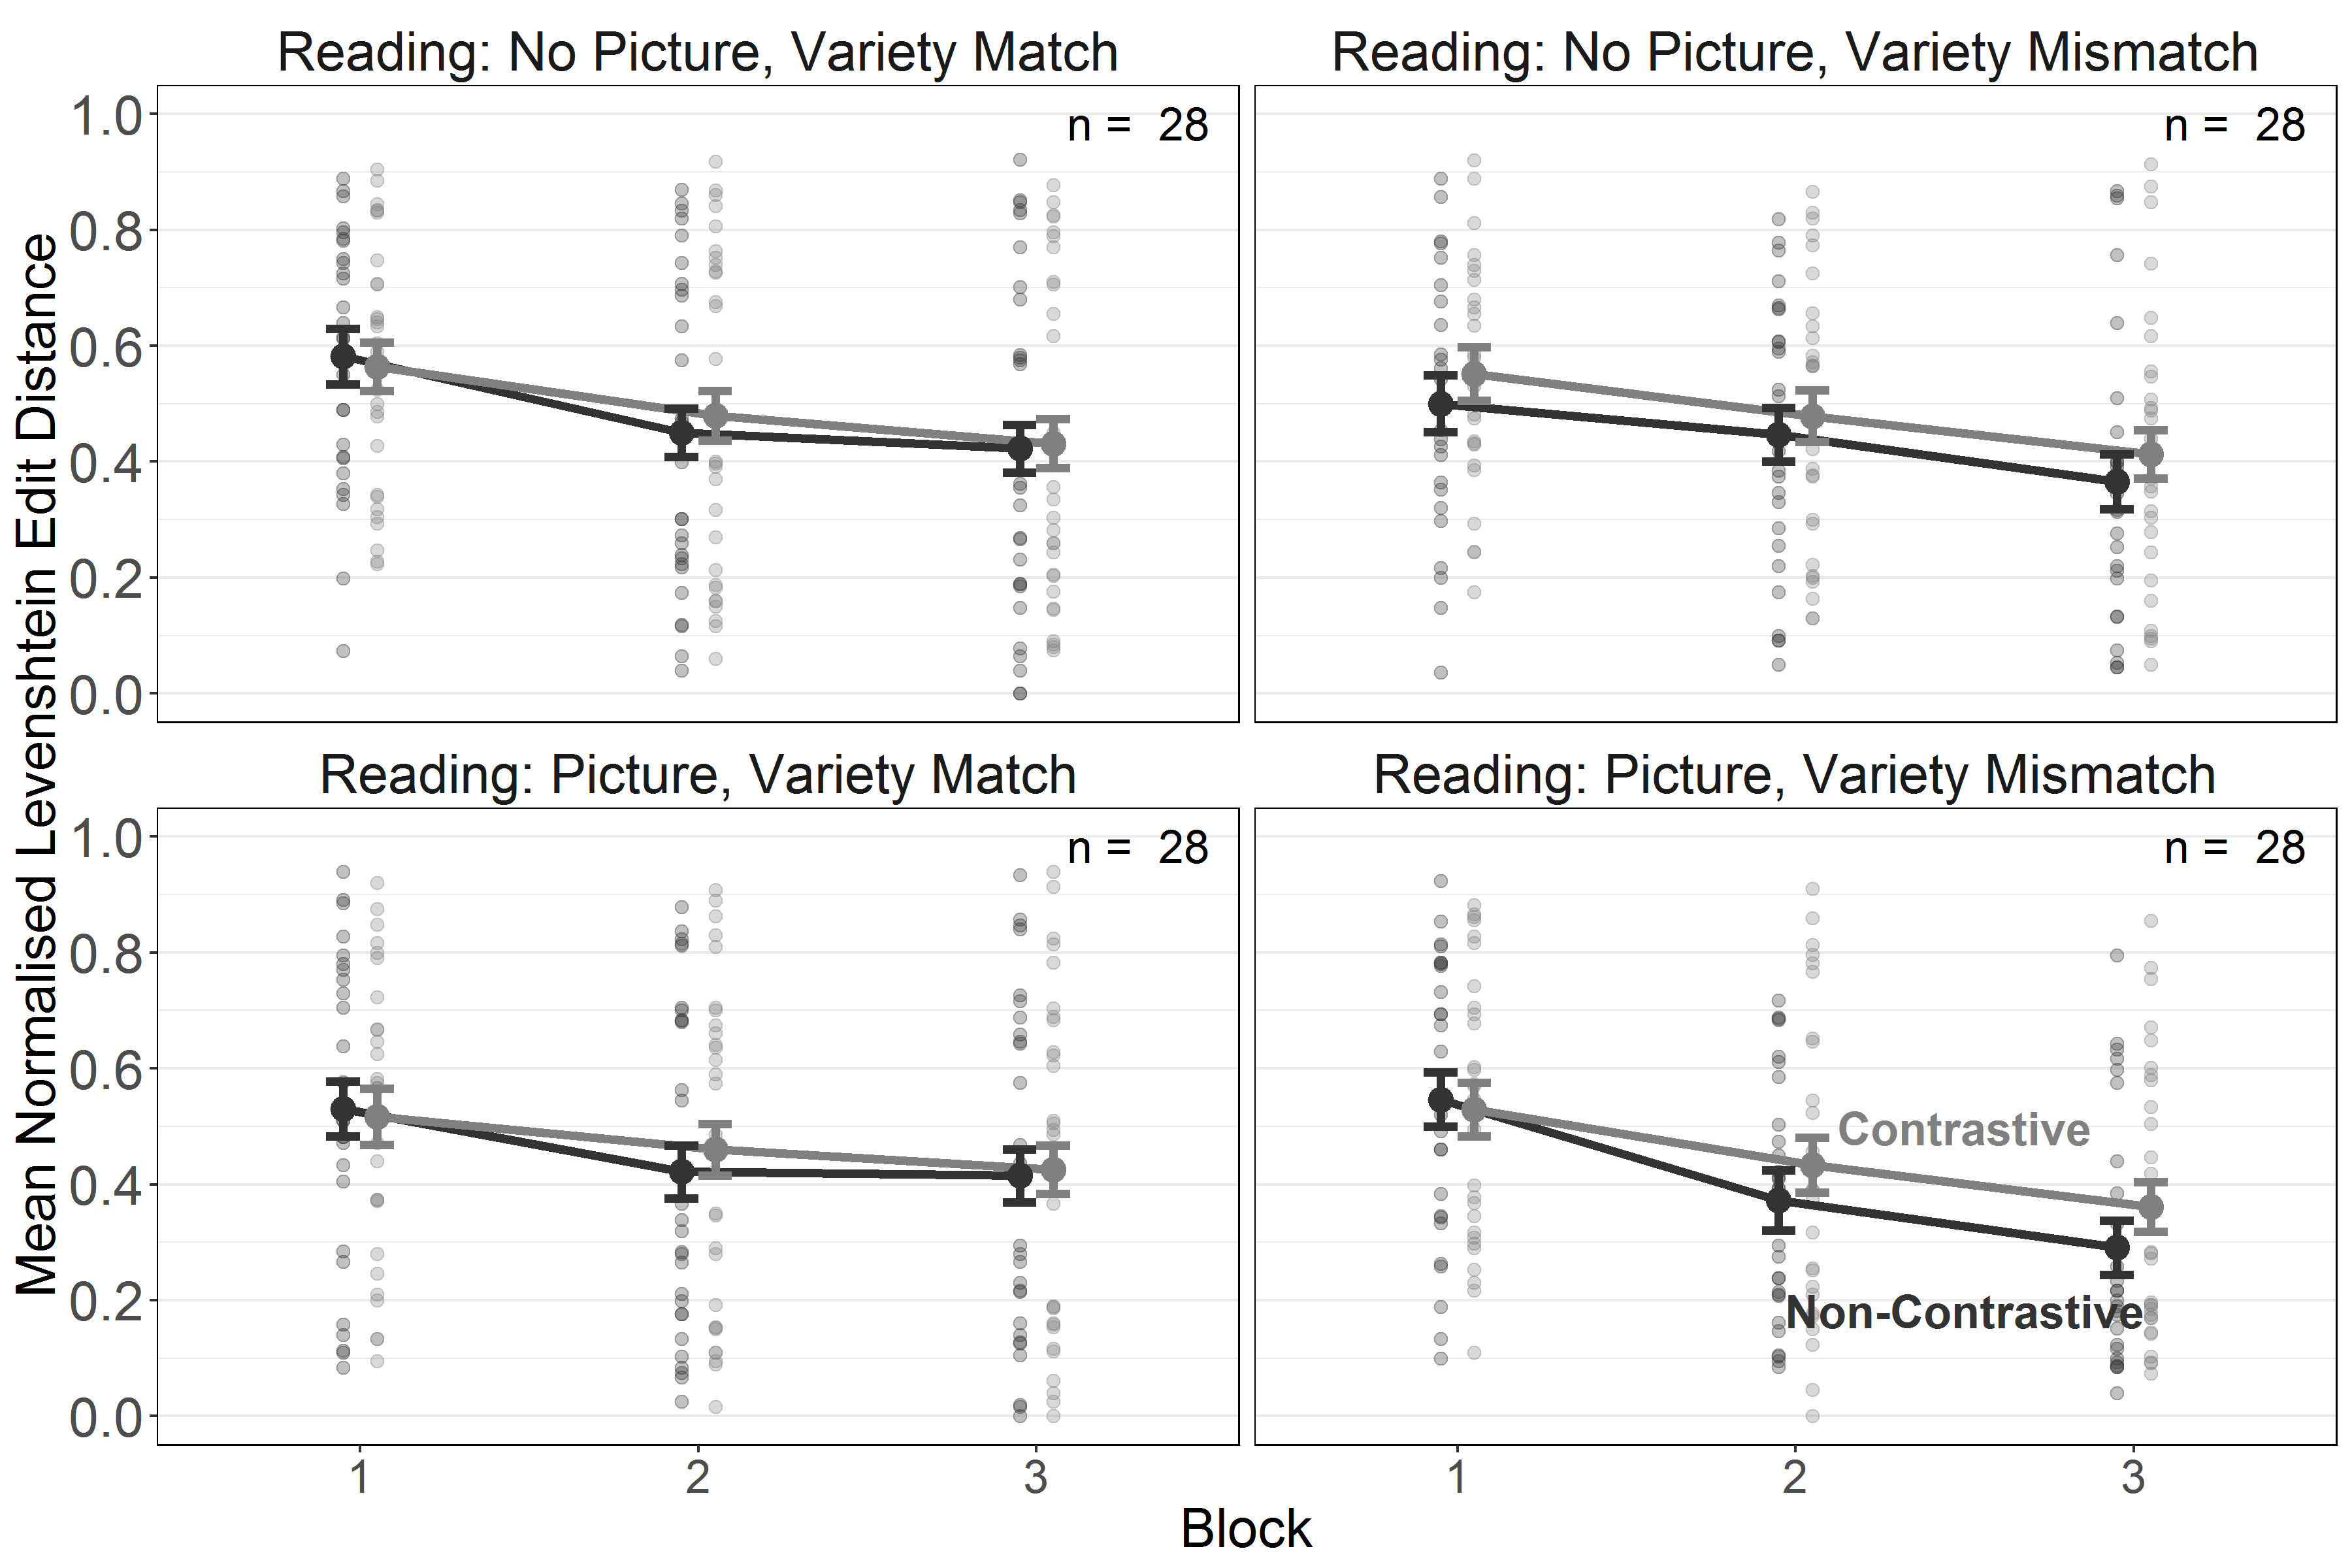
\includegraphics[width=1\linewidth]{C:/Users/g517364/Dropbox/GitHub/levenik/04_figures/output/experiment-0_training_plot_reading} 

}

\caption{Experiment 1. Length-normalised Levenshtein Edit Distance for reading training of contrastive and non-contrastive words over 3 double-blocks (coded as 6 blocks in the analyses but presented as 3 double-blocks for comparability with Experiment 2) in the variety match and mismatch conditions. Error bars indicate $\pm$ 1 $SE$ of the mean.}\label{fig:ex0-train-plots}
\end{figure}

\paragraph{Testing}\label{testing}

For the analysis of the testing phase, we used the same fixed effect
structure as for the analysis of the training phase with the exclusion
of the linear and quadratic effects of Block. The only difference was
that here Word Type was modelled using Helmert contrasts, such that
contrastive words were compared to non-contrastive words and untrained
words were compared to the average of contrastive and non-contrastive
words (i.e.~the trained words). For the testing phase, the random
effects structure included random intercepts and slopes of Picture
Condition, Language Variety, and their interaction by items, and random
intercepts and slopes of Word Type by subjects.

\begin{table}[!h]

\caption{\label{tab:ex0-test}Experiment 1. Parameter estimates for the models fitted to nLEDs from the testing phase. Bayesian analyses report standardised parameter estimates (i.e. the intercept [grand mean] is centred at 0). Values of 0 with a sign indicate the direction of the estimate before rounding.}
\centering
\resizebox{\linewidth}{!}{
\fontsize{8}{10}\selectfont
\begin{tabular}{lrrlrlrrl}
\toprule
\multicolumn{1}{c}{ } & \multicolumn{5}{c}{Frequentist Estimates} & \multicolumn{3}{c}{Bayesian Estimates} \\
\cmidrule(l{3pt}r{3pt}){2-6} \cmidrule(l{3pt}r{3pt}){7-9}
Term & $Est.$ & $SE$ & 95\% Conf. I & $t$ & $p$ & $Est.$ & $SE$ & 95\% Cred. I\\
\midrule
Intercept & 0.61 & 0.04 & [0.54, 0.68] & 16.15 & < .001*** & 0.01 & 0.08 & [-0.14, 0.19]\\
Picture Condition & 0.04 & 0.04 & [-0.03, 0.11] & 1.06 & < .001*** & 0.06 & 0.07 & [-0.08, 0.20]\\
Variety Condition & -0.05 & 0.04 & [-0.12, 0.02] & -1.33 & < .001*** & -0.08 & 0.07 & [-0.21, 0.07]\\
PC $\times$ VC & 0.02 & 0.04 & [-0.05, 0.09] & 0.64 & 1.00 & 0.04 & 0.07 & [-0.09, 0.18]\\
NP, VMis: WT & -0.02 & 0.02 & [-0.05, 0.01] & -1.13 & < .001*** & -0.03 & 0.03 & [-0.10, 0.03]\\
P, VMis: WT & -0.03 & 0.02 & [-0.07, -0.00] & -2.00 & < .001*** & -0.07 & 0.03 & [-0.13, -0.00]\\
NP, VMa: WT & 0.00 & 0.02 & [-0.04, 0.04] & 0.02 & 1.00 & 0.00 & 0.03 & [-0.07, 0.07]\\
P, VMa: WT & 0.00 & 0.02 & [-0.03, 0.03] & -0.23 & 1.00 & -0.01 & 0.03 & [-0.07, 0.06]\\
NP, VMis, WF & 0.01 & 0.01 & [-0.02, 0.04] & 0.74 & < .001*** & 0.02 & 0.03 & [-0.04, 0.08]\\
P, VMis, WF & 0.03 & 0.01 & [-0.00, 0.06] & 1.94 & < .001*** & 0.06 & 0.03 & [0.00, 0.12]\\
NP, VMa, WF & 0.01 & 0.02 & [-0.03, 0.04] & 0.32 & 1.00 & 0.01 & 0.03 & [-0.05, 0.07]\\
\textbf{P, VMa, WF} & \textbf{0.04} & \textbf{0.01} & \textbf{[0.01, 0.07]} & \textbf{2.85} & \textbf{< .001***} & \textbf{0.08} & \textbf{0.03} & \textbf{[0.02, 0.14]}\\
\bottomrule
\multicolumn{9}{l}{Variety Condition (VC) = variety match vs. variety mismatch (VMa vs. VMi),}\\
\multicolumn{9}{l}{Picture Condition (PC) = picture vs. no picture (P vs. NP),}\\
\multicolumn{9}{l}{Word Type (WT) = contrastive vs. non-contrastive, Word Familiarity (WF) = familiar vs. unfamiliar (novel)}\\
\end{tabular}}
\end{table}

We found that the contrastive deficit failed to reach significance in
the Variety Mismatch condition. The effect of Word Familiarity was
significant in the Variety Match condition with pictures and fell short
of significance in the Variety Mismatch condition with pictures
suggesting that when pictures were present allowing for establishment of
links between word form and meaning phonological decoding skills were
applied insufficiently as participants were more likely to access the
phonological form via a word's meaning rather than applying
grapheme-phoneme conversion rules.

We performed a planned direct comparison of performance on untrained
words only between the Variety Match and Variety Mismatch conditions.
The model included fixed effects and interactions between the sum-coded
Picture Condition and Language Variety. We used the same criteria as in
our main models for determining the random effects structure of the
model. Here, this took the form of random zero-correlation intercepts
and slopes of Picture Condition and Language Variety and their
interaction by items, and random intercepts by subjects.

This comparison showed no effect of variety mismatch (frequentist
estimate: \(\hat{\beta}\) = -0.05{[}-0.13, 0.03{]}, \emph{t} = -1.21,
\emph{p} = \textless{} .001***; Bayesian Estimate: \(\hat{\beta}\) =
-0.09{[}-0.26, 0.07{]}), thus failing to obtain conclusive evidence for
a detrimental effect of dialect exposure on phonological decoding
skills.

\begin{figure}[htb]

{\centering 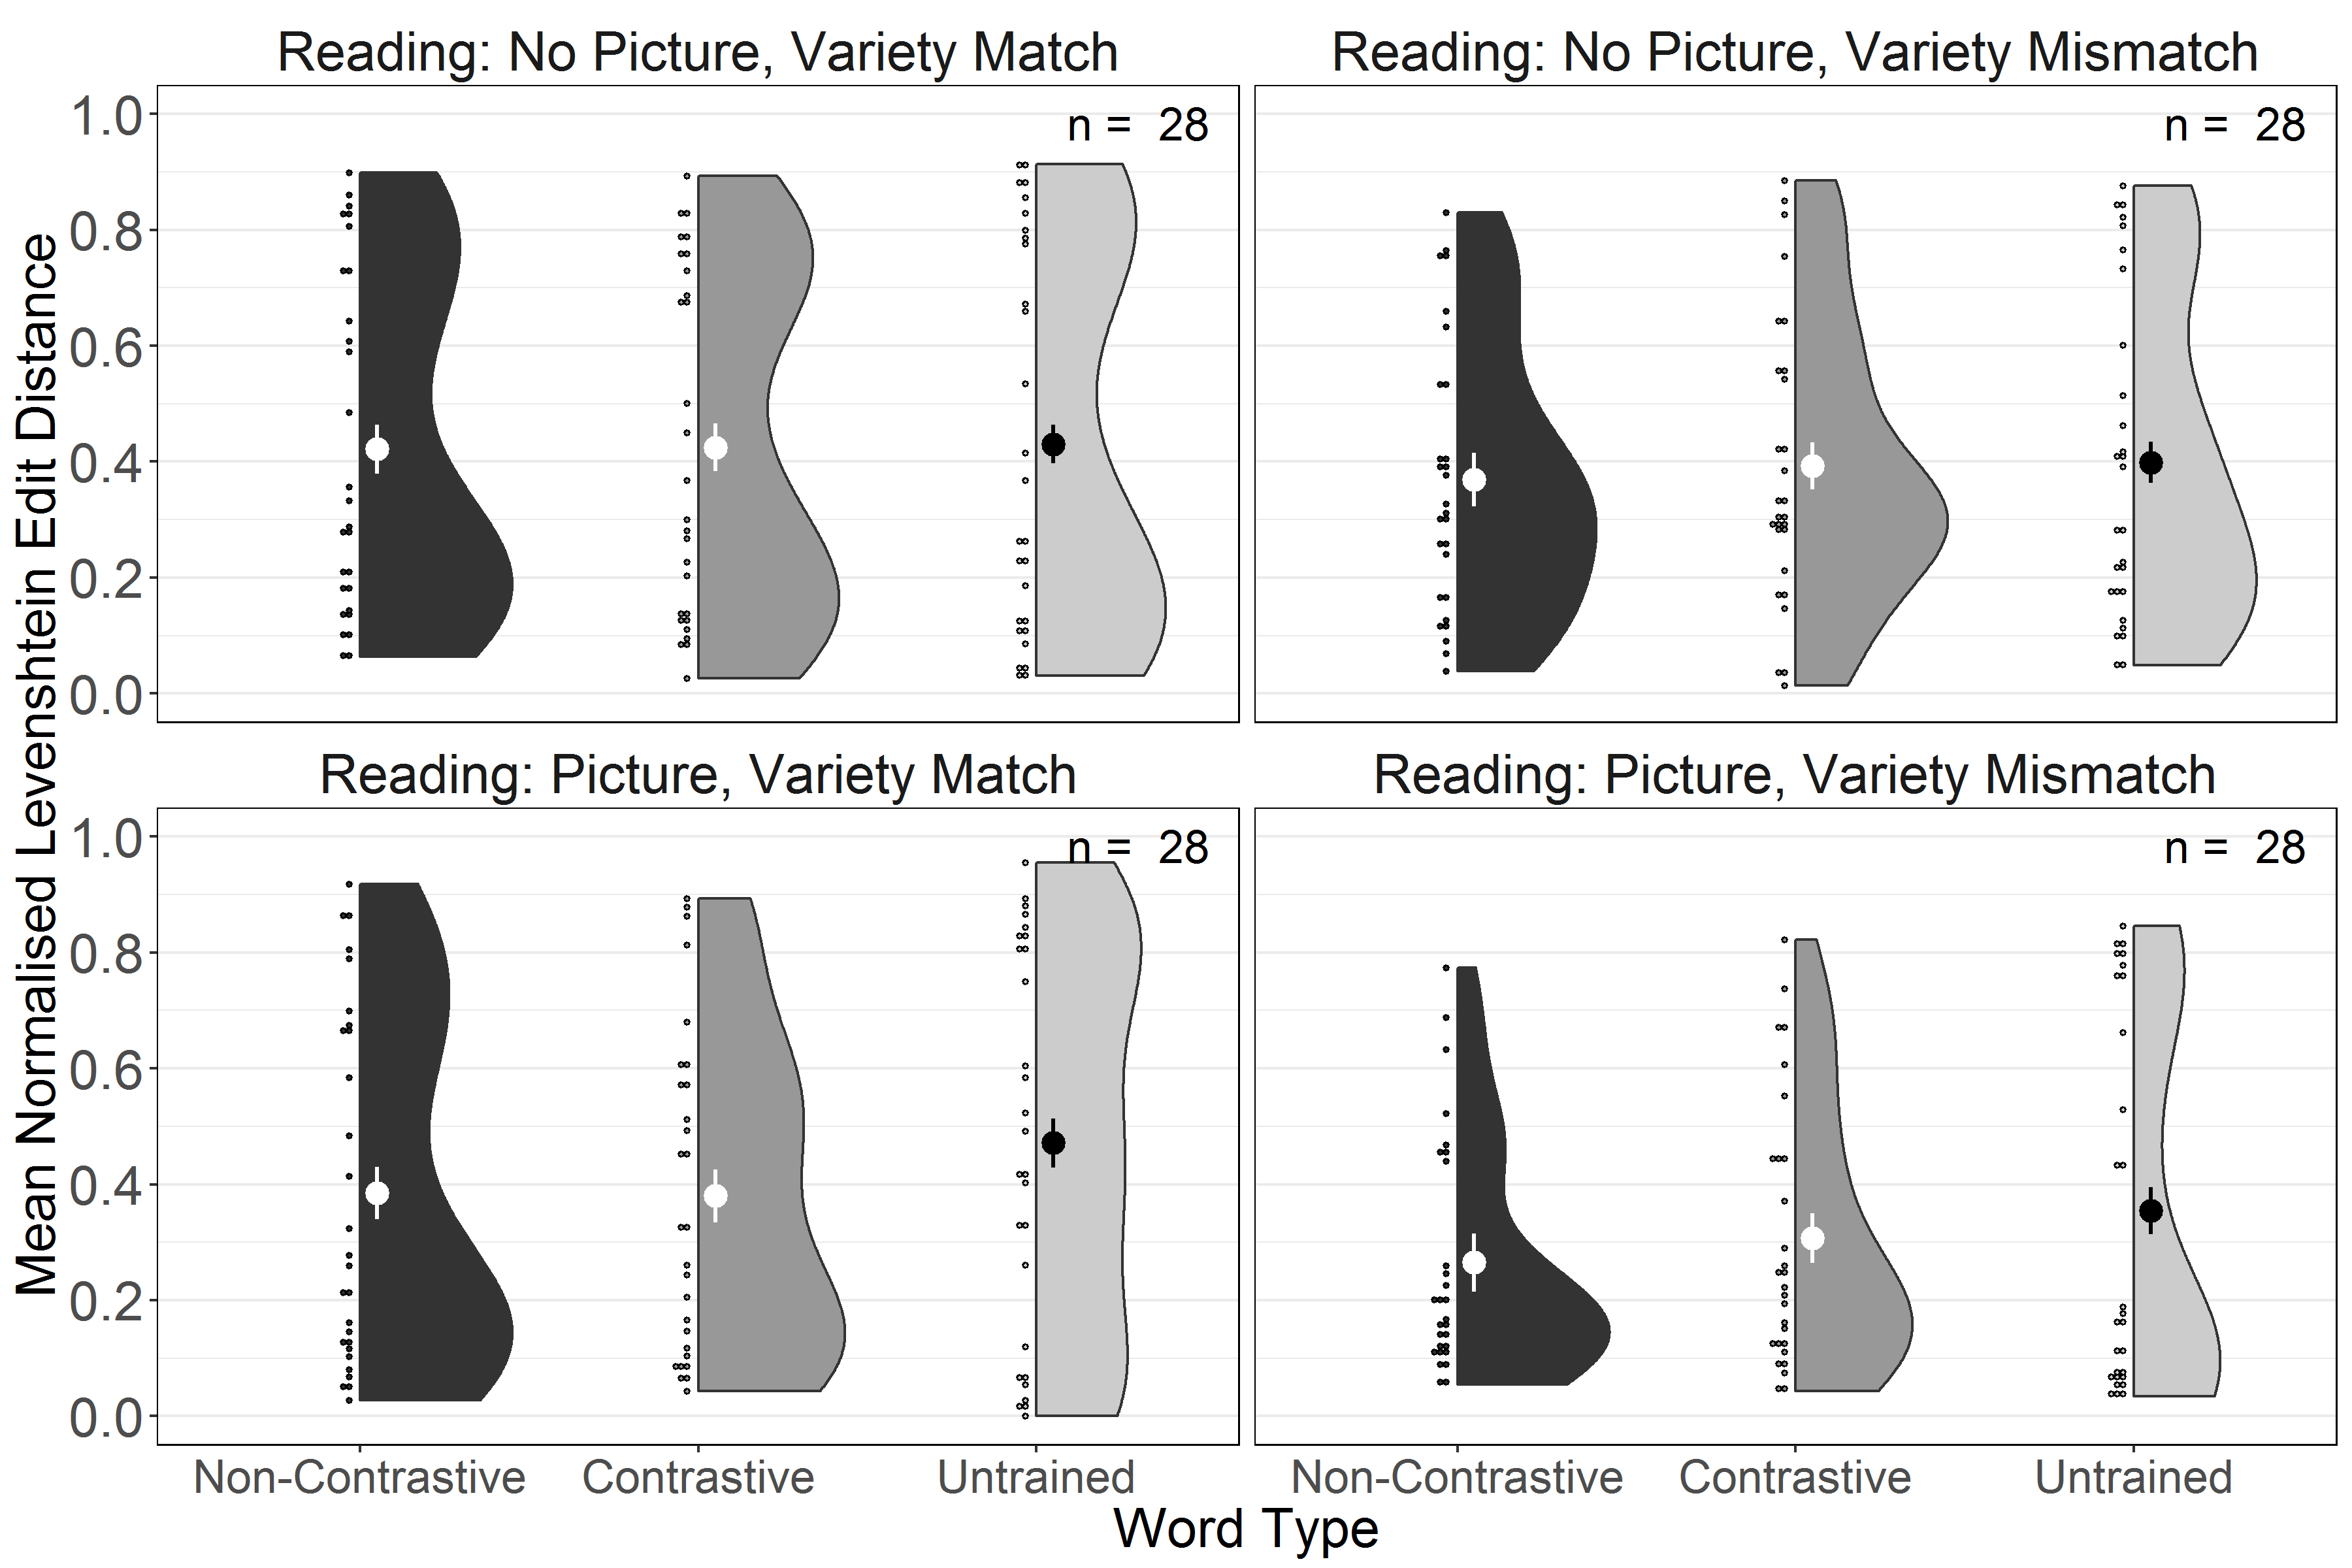
\includegraphics[width=1\linewidth]{C:/Users/g517364/Dropbox/GitHub/levenik/04_figures/output/experiment-0_testing_plot_reading} 

}

\caption{Experiment 1. Length-normalised Levenshtein Edit Distance for reading testing of trained non-contrastive, trained contrastive and untrained words in the variety match and variety mismatch conditions. Large dots and whiskers indicate means and $\pm$ 1 $SE$ of the mean.}\label{fig:ex0-test-plots}
\end{figure}

\subsection{Discussion}\label{discussion}

In this experiment, participants learned to read 30 words of an
artificial language using an artificial script. One group learned to
read the same variants as they had encountered during exposure while for
the other group half of the words varied between exposure and literacy
acquisition mimicking a situation of dialect exposure. Orthogonal to the
manipulation of Variety Mismatch, half of the participants saw pictures
when hearing the words enabling them to develop semantic representations
while the other half did not. Reading performance improved significantly
over the course of training in both the variety match and mismatch
conditions although the gains were steeper in the Variety Mismatch
condition with pictures. We had predicted that performance would be
worse for contrastive compared to non-contrastive words in the variety
mismatch condition. While the results confirmed this trend, the
contrastive deficit only reached significance during training in the No
Picture condition, in line with findings from the reading experiment and
the connectionist simulation of exposure to AAE by Brown et al. (2015).
However, in that simulation the contrastive deficit arose solely from
similarity between the phonological representations of the AAE and MAE
variants and not from competition between word forms associated with the
same concept. Our experiment was not able to unequivocally establish the
role of semantic representations on the magnitude of the contrastive
deficit as we only observed it in the No Picture condition during
training but not reliably during testing. It should be noted, however,
that participants displayed extraordinary variability due to the
considerable difficulty of the task. Thus, our results remain equivocal
with respect to whether contrastive deficits persist when semantic
representations are being established.

To the extent that beginning readers rely on direct associations between
print and meaning the encounter of untrained words should disrupt
performance as phonologically mediated decoding skills need to be
employed. The Word Familiarity effect is therefore a measure for how
reliably such grapheme-phoneme conversion rules have been acquired. In
this experiment, reduced performance with untrained, and hence
unfamiliar, words was only observed in the variety match condition with
pictures. This suggests that when no competing variants were present in
the input and semantic information was available learners may have
attempted to memorise the direct associations between the orthographic
and the phonological form of a word. It should be noted that there was
also a marginal effect of word familiarity when pictures were provided
in the variety mismatch condition confirming that availability of
semantic information in general encouraged a strategy of establishing
direct associations between meanings and phonological forms rather than
trying to retrieve the sound based decoding of the orthographical form.
There was no word familiarity effect in the No Picture conditions
because attempting to forge direct links between graphemic and phonemic
representations that bypass decoding in the absence of semantic cues is
extremely difficult.

The crucial question was whether exposure to competing variants would
affect learners emerging phonological decoding skills. To answer this
question, we compared reading performance for untrained words between
the Variety Match and Mismatch conditions. If dialect exposure hinders
literacy acquisition as suspected by the Head Teacher mentioned in our
introductory paragraph we would expect poorer performance with untrained
words in the variety mismatch condition, yet the comparison of reading
performance of untrained words showed no difference to the variety match
condition. However, Bayesian analyses designed to estimate the strength
of evidence for the null hypothesis indicated that there was
insufficient evidence for lack of an effect. We therefore can neither
confirm nor exclude the possibility that dialect exposure impairs
decoding skills.

One possible reason for this result is that the absence of spelling
training may have prevented participants from attempting to convert
graphemes into phonemes. However, beginning readers never learn to read
only but also learn to spell as primary schools tend to incorporate
writing instruction into their curricula from early on (Cutler \&
Graham, 2008). Spelling training strengthens the connections between
individual phonemes and graphemes thereby promoting use of decoding
skills. For example, Taylor et al. (2017) showed that included a
spelling task into the training regimen for an artificial script
encouraged a phonologically-mediated reading acquisition strategy. While
the child participants in the Brown et al. (2015) study would certainly
have engaged in spelling practice during their schooling, the
corresponding neural network did not include bi-directional links that
could have instantiated a \enquote{spelling path}, i.e.~a path from
phonological to graphemic representations (see Houghton \& Zorzi, 2003),
and we are not aware of any attempts to computationally model to
contribution of spelling practice to emergent reading skills. Thus, it
is not clear whether under conditions that encourage decoding skills
like spelling practice detrimental effects of dialect exposure should be
expected.

In this experiment, using grapheme-phoneme conversion rules had also
been made difficult by the opaque spelling system that was designed to
mimic the acquisition of a deep orthography like English. Recall that we
implemented two conditional rules where grapheme-phoneme associations
changed depending on orthographic context. This complex conditional rule
system is likely to have further discouraged discovery and use of
grapheme-phoneme conversion rules. To promote learning of these rules
and to encourage phonologically-mediated reading, we presented a
transparent orthography in Experiment 2a and the opaque orthography from
Experiment 1 in Experiment 2b. The comparison will be instructive for
trying to understand the potential role of dialect exposure in languages
with a more shallow orthography, such as, for example, the effect of
exposure to Swiss German on acquiring literacy in Standard German.

\section{Experiment 2: Effect of variety mismatch on learning to read
and
spell}\label{experiment-2-effect-of-variety-mismatch-on-learning-to-read-and-spell}

The aim of Experiment 2 was to provide more ecologically valid training
conditions by examining the effect of exposure to variety mismatch when
participants learned to read and to spell a transparent (Experiment 2a)
and an opaque (Experiment 2b) orthography.

\section{Experiment 2a: Transparent
Orthography}\label{experiment-2a-transparent-orthography}

\subsection{Method}\label{method-1}

\subsubsection{Participants}\label{participants-1}

One hundred and twelve participants (aged 20--65, aged \emph{M} = 36.73,
\emph{SD} = 10.67) were recruited from Amazon's Mechanical Turk and took
part in the study for \$7.50. All participants reported proficiency in
English (1-7 Likert scale: \emph{M} = 4.90, \emph{SD} = 0.40). Another 2
participants were tested and excluded based on the exclusion criteria
described for Experiment 1.

\subsubsection{Materials}\label{materials-1}

We used the same set of graphemes, phonemes and words as in Experiment
1. In contrast to Experiment 1, we adopted only one-to-one mappings
between graphemes and phonemes resulting in an entirely transparent,
shallow orthography.

\subsubsection{Procedure}\label{procedure-1}

The procedure was identical to Experiment 1 aside from the following
deviation: In the training phase that followed exposure to the
grapheme-phoneme mappings, each ten-word block was presented twice, once
for reading training and once for spelling training. During spelling
training participants heard a word and had to type it by clicking
graphemes using an on-screen keyboard. Participants in the Picture
condition always saw the picture of the associated referent when hearing
the word. Once participants had pressed the on-screen \enquote{Enter}
key the correct spelling appeared below their own spelling for purposes
of feedback. The screen was cleared after 1.5 to 3.0 sec to prevent
participants to take notes or obtain screenshots (the exact time was
determined dynamically based on the word length, where for each letter
the duration would last for an additional 500ms). The overall amount of
exposure to each item, combining presentations for reading and spelling,
was identical to Experiment 1. In the testing phase, participants were
presented with all thirty training words and an additional twelve
untrained words in randomised order. Just as the training phase, the
testing phase also contained both a reading and a spelling stage. Order
of reading and spelling task was counterbalanced across participants but
was kept constant across all phases within participants. The mean
completion time was 63.88 minutes (\emph{SD} = 23.00). An example of the
experimental procedure can be found at
\url{https://language.abertay.ac.uk/allp-demo/}.

\subsection{Results}\label{results-1}

\subsubsection{Coding}\label{coding-1}

We used the same coding scheme for reading responses as in Experiment 1.
The ICC between coders was F(16113.00, 11887.47) = 84.39, \(p\)
\textless{} .001, ICC = 0.98 {[}95\% CI = 0.98; 0.98{]}. The 95\%
confidence interval around the parameter estimate indicates that the ICC
falls above the bound of .90, which suggests excellent reliability
across raters (see Koo \& Li, 2016).

\subsubsection{Model Fitting}\label{model-fitting-1}

Model fitting was similar to Experiment 1, with the exception of the
inclusion of a sum-coded fixed effect of Task (reading vs.~spelling) and
inclusion of Task in the random effects for the analyses of the training
and testing data. Additionally, since the training phase contained 3
blocks of training for each task, the training models were changed to
include only an orthogonal linear (and not quadratic) time term as a
fixed and random effect. This change was made to avoid overfitting for
change over time with only 3 time points. As in Experiment 1, the fixed
effects for training and testing data were modelled with a nested
structure, with Word Type nested within all other factors (i.e.~Task,
Variety Condition, Picture Condition in both phases, and with the
addition of the orthogonal linear effect of time in the training phase).
Thus, we obtained all main effects and interactions between all factors
excluding Word Type, and simple effects of Word Type within each
combination of the levels for the other factors.

For the training phase, the maximal converging random effects structure
took the form of zero-correlation random intercepts and slopes of Task,
Picture Condition, Variety Condition, and their interaction by items,
and zero-correlation random intercepts and slopes for the linear time
term, Task, Word Type, and their interaction by subjects. For the
testing phase, the random effects structure took the form of random
intercepts and slopes of Task, Picture Condition, Variety Condition, and
their interaction by items, and random intercepts and slopes for Task,
Word Type, and their interaction by subjects (including correlations
between all terms for both by-items and by-subjects random effects).

As with Experiment 1, we also modelled the data using Bayesian mixed
effects models with a maximal random effects structure. These models
used the same priors as in Experiment 1, with the addition of
informative, \(Normal(0, 0.2)\) priors on the fixed effect of Task and
any interactions of other terms with this factor. We used these models
to evaluate evidence in support of the null hypothesis for each
parameter using in the same way as in Experiment 1.

\paragraph{Training}\label{training-1}

Parameter estimates, confidence intervals (for the frequentist analysis)
and credible intervals (for the Bayesian analysis) are presented in
Table~\ref{tab:ex1-train} and depicted in
Figures~\ref{fig:ex1-train-reading-plots} and
\ref{fig:ex1-train-spelling-plots}.

\begin{table}[!h]

\caption{\label{tab:ex1-train}Experiment 2a. Parameter estimates for the models fitted to nLEDs from the training phase. Bayesian analyses report standardised parameter estimates (i.e. the intercept [grand mean] is centred at 0). Values of 0 with a sign indicate the direction of the estimate before rounding.}
\centering
\resizebox{\linewidth}{!}{
\fontsize{8}{10}\selectfont
\begin{tabular}{lrrlrlrrl}
\toprule
\multicolumn{1}{c}{ } & \multicolumn{5}{c}{Frequentist Estimates} & \multicolumn{3}{c}{Bayesian Estimates} \\
\cmidrule(l{3pt}r{3pt}){2-6} \cmidrule(l{3pt}r{3pt}){7-9}
Term & $Est.$ & $SE$ & 95\% Conf. I & $t$ & $p$ & $Est.$ & $SE$ & 95\% Cred. I\\
\midrule
Intercept & 0.66 & 0.04 & [0.59, 0.73] & 18.67 & < .001*** & 0.00 & 0.07 & [-0.15, 0.14]\\
\textbf{Block} & \textbf{-8.92} & \textbf{0.77} & \textbf{[-10.44, -7.40]} & \textbf{-11.51} & \textbf{< .001***} & \textbf{-0.37} & \textbf{0.03} & \textbf{[-0.44, -0.31]}\\
\textbf{Task} & \textbf{-0.04} & \textbf{0.01} & \textbf{[-0.06, -0.03]} & \textbf{-5.16} & \textbf{< .001***} & \textbf{-0.09} & \textbf{0.02} & \textbf{[-0.12, -0.05]}\\
Picture Condition & 0.05 & 0.03 & [-0.02, 0.11] & 1.33 & < .001*** & 0.08 & 0.07 & [-0.05, 0.21]\\
Variety Condition & -0.05 & 0.03 & [-0.12, 0.02] & -1.43 & < .001*** & -0.09 & 0.07 & [-0.21, 0.04]\\
B $\times$ TC & -0.39 & 0.39 & [-1.15, 0.38] & -0.99 & < .001*** & -0.02 & 0.02 & [-0.05, 0.02]\\
B $\times$ PC & -0.27 & 0.77 & [-1.79, 1.25] & -0.35 & 1.00 & -0.01 & 0.03 & [-0.08, 0.05]\\
TC $\times$ PC & 0.00 & 0.01 & [-0.02, 0.01] & -0.48 & 1.00 & -0.01 & 0.02 & [-0.04, 0.02]\\
B $\times$ VC & 0.90 & 0.77 & [-0.62, 2.42] & 1.16 & < .001*** & 0.04 & 0.03 & [-0.03, 0.10]\\
TC $\times$ VC & -0.01 & 0.01 & [-0.02, 0.01] & -1.19 & < .001*** & -0.02 & 0.02 & [-0.05, 0.01]\\
PC $\times$ VC & -0.02 & 0.03 & [-0.09, 0.05] & -0.55 & 1.00 & -0.03 & 0.07 & [-0.16, 0.10]\\
B $\times$ TC $\times$ PC & -0.18 & 0.39 & [-0.94, 0.58] & -0.46 & 1.00 & -0.01 & 0.02 & [-0.04, 0.02]\\
B $\times$ TC $\times$ VC & 0.01 & 0.39 & [-0.75, 0.77] & 0.02 & 1.00 & 0.00 & 0.02 & [-0.03, 0.03]\\
B $\times$ PC $\times$ VC & -1.43 & 0.77 & [-2.95, 0.09] & -1.85 & < .001*** & -0.06 & 0.03 & [-0.12, 0.01]\\
TC $\times$ PC $\times$ VC & 0.00 & 0.01 & [-0.01, 0.02] & 0.63 & 1.00 & 0.01 & 0.02 & [-0.02, 0.04]\\
B $\times$ TC $\times$ PC $\times$ VC & -0.58 & 0.39 & [-1.34, 0.18] & -1.49 & < .001*** & -0.02 & 0.02 & [-0.06, 0.01]\\
\textbf{R, NP, VMis: WT} & \textbf{-0.04} & \textbf{0.01} & \textbf{[-0.07, -0.01]} & \textbf{-2.47} & \textbf{< .001***} & \textbf{-0.07} & \textbf{0.03} & \textbf{[-0.13, -0.01]}\\
S, NP, VMis: WT & 0.00 & 0.01 & [-0.03, 0.03] & 0.27 & 1.00 & 0.01 & 0.03 & [-0.05, 0.07]\\
\textbf{R, P, VMis: WT} & \textbf{-0.05} & \textbf{0.01} & \textbf{[-0.08, -0.02]} & \textbf{-3.60} & \textbf{< .001***} & \textbf{-0.10} & \textbf{0.03} & \textbf{[-0.16, -0.04]}\\
S, P, VMis: WT & -0.01 & 0.01 & [-0.04, 0.02] & -0.67 & 1.00 & -0.02 & 0.03 & [-0.07, 0.04]\\
R, NP, VMa: WT & -0.01 & 0.01 & [-0.04, 0.01] & -0.99 & < .001*** & -0.02 & 0.03 & [-0.08, 0.04]\\
S, NP, VMa: WT & -0.01 & 0.01 & [-0.04, 0.02] & -0.55 & 1.00 & -0.01 & 0.03 & [-0.07, 0.04]\\
R, P, VMa: WT & 0.00 & 0.01 & [-0.03, 0.03] & -0.02 & 1.00 & 0.00 & 0.03 & [-0.06, 0.06]\\
S, P, VMa: WT & -0.01 & 0.01 & [-0.04, 0.02] & -0.49 & 1.00 & -0.01 & 0.03 & [-0.07, 0.05]\\
B, R, NP, VMis: WT & -0.18 & 0.90 & [-1.95, 1.59] & -0.20 & 1.00 & -0.01 & 0.04 & [-0.09, 0.07]\\
B, S, NP, VMis: WT & -0.43 & 0.90 & [-2.21, 1.34] & -0.48 & 1.00 & -0.02 & 0.04 & [-0.09, 0.05]\\
\textbf{B, R, P, VMis: WT} & \textbf{-2.21} & \textbf{0.90} & \textbf{[-3.97, -0.45]} & \textbf{-2.46} & \textbf{< .001***} & \textbf{-0.09} & \textbf{0.04} & \textbf{[-0.16, -0.02]}\\
B, S, P, VMis: WT & -0.96 & 0.90 & [-2.72, 0.80] & -1.07 & < .001*** & -0.04 & 0.04 & [-0.11, 0.04]\\
B, R, NP, VMa: WT & -0.25 & 0.90 & [-2.02, 1.51] & -0.28 & 1.00 & -0.01 & 0.04 & [-0.08, 0.06]\\
B, S, NP, VMa: WT & 0.55 & 0.90 & [-1.22, 2.32] & 0.61 & 1.00 & 0.02 & 0.04 & [-0.05, 0.10]\\
B, R, P, VMa: WT & -0.14 & 0.90 & [-1.91, 1.63] & -0.15 & 1.00 & -0.01 & 0.04 & [-0.08, 0.06]\\
B, S, P, VMa: WT & 1.03 & 0.90 & [-0.75, 2.80] & 1.13 & < .001*** & 0.04 & 0.04 & [-0.03, 0.12]\\
\bottomrule
\multicolumn{9}{l}{Block (B) = 1-3, Variety Condition (VC) = variety match vs. variety mismatch (VMa vs. VMi),}\\
\multicolumn{9}{l}{Picture Condition (PC) = picture vs. no picture (P vs. NP), Task Condition (TC) = reading vs. spelling (R vs. S),}\\
\multicolumn{9}{l}{Word Type (WT) = contrastive vs. non-contrastive}\\
\end{tabular}}
\end{table}

The results showed a main effect of Block, indicating an overall
improvement of performance as training progressed, as well as a main
effect of Task demonstrating better performance for reading than for
spelling. Crucially, we found that reading, but not spelling, of
contrastive words, as indicated by the effect of Word Type, was
significantly impaired in the Variety Mismatch condition regardless of
Picture condition. In the Picture condition, the effect of Word Type in
reading in the Variety Mismatch condition interacted with Block
reflecting the fact that impaired performance for contrastive words
started to manifest itself gradually over the course of training.

\begin{figure}[htb]

{\centering 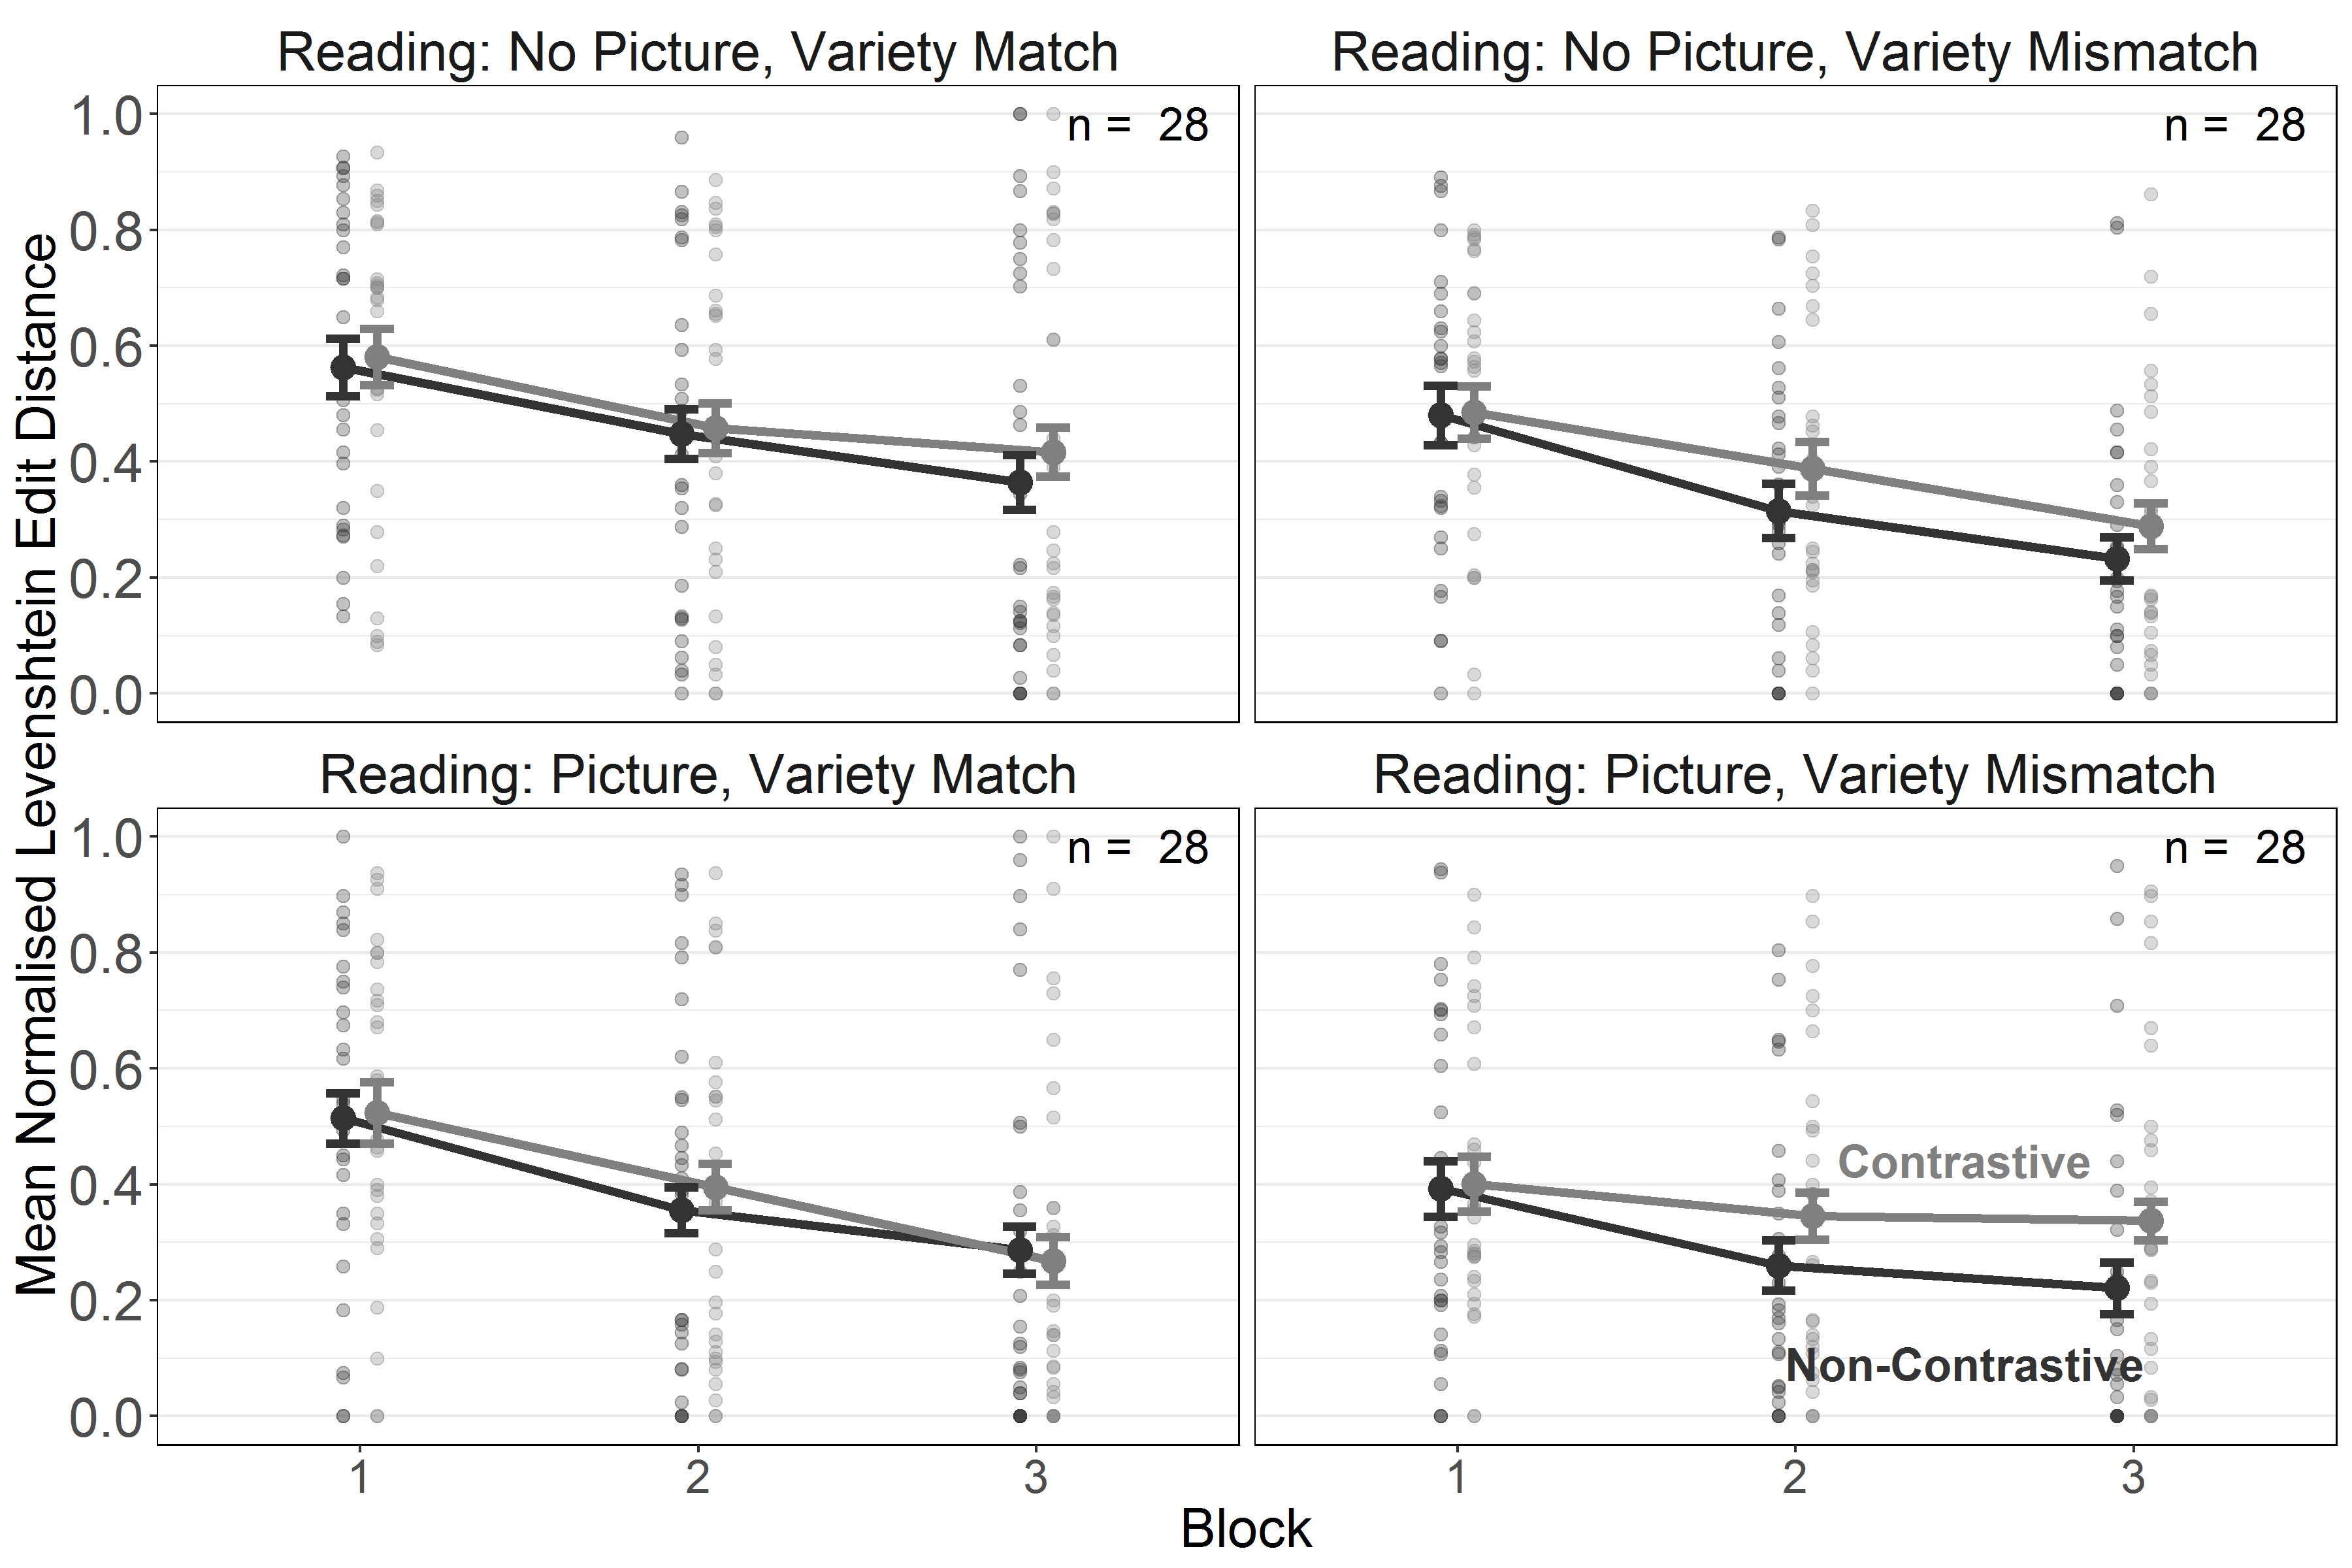
\includegraphics[width=1\linewidth]{C:/Users/g517364/Dropbox/GitHub/levenik/04_figures/output/experiment-1_training_plot_reading} 

}

\caption{Experiment 2a. Length-normalised Levenshtein Edit Distance for reading of contrastive and non-contrastive words during 3 training blocks in the variety match and variety mismatch conditions. Error bars indicate $\pm$ 1 $SE$ of the mean.}\label{fig:ex1-train-reading-plots}
\end{figure}

\begin{figure}[htb]

{\centering 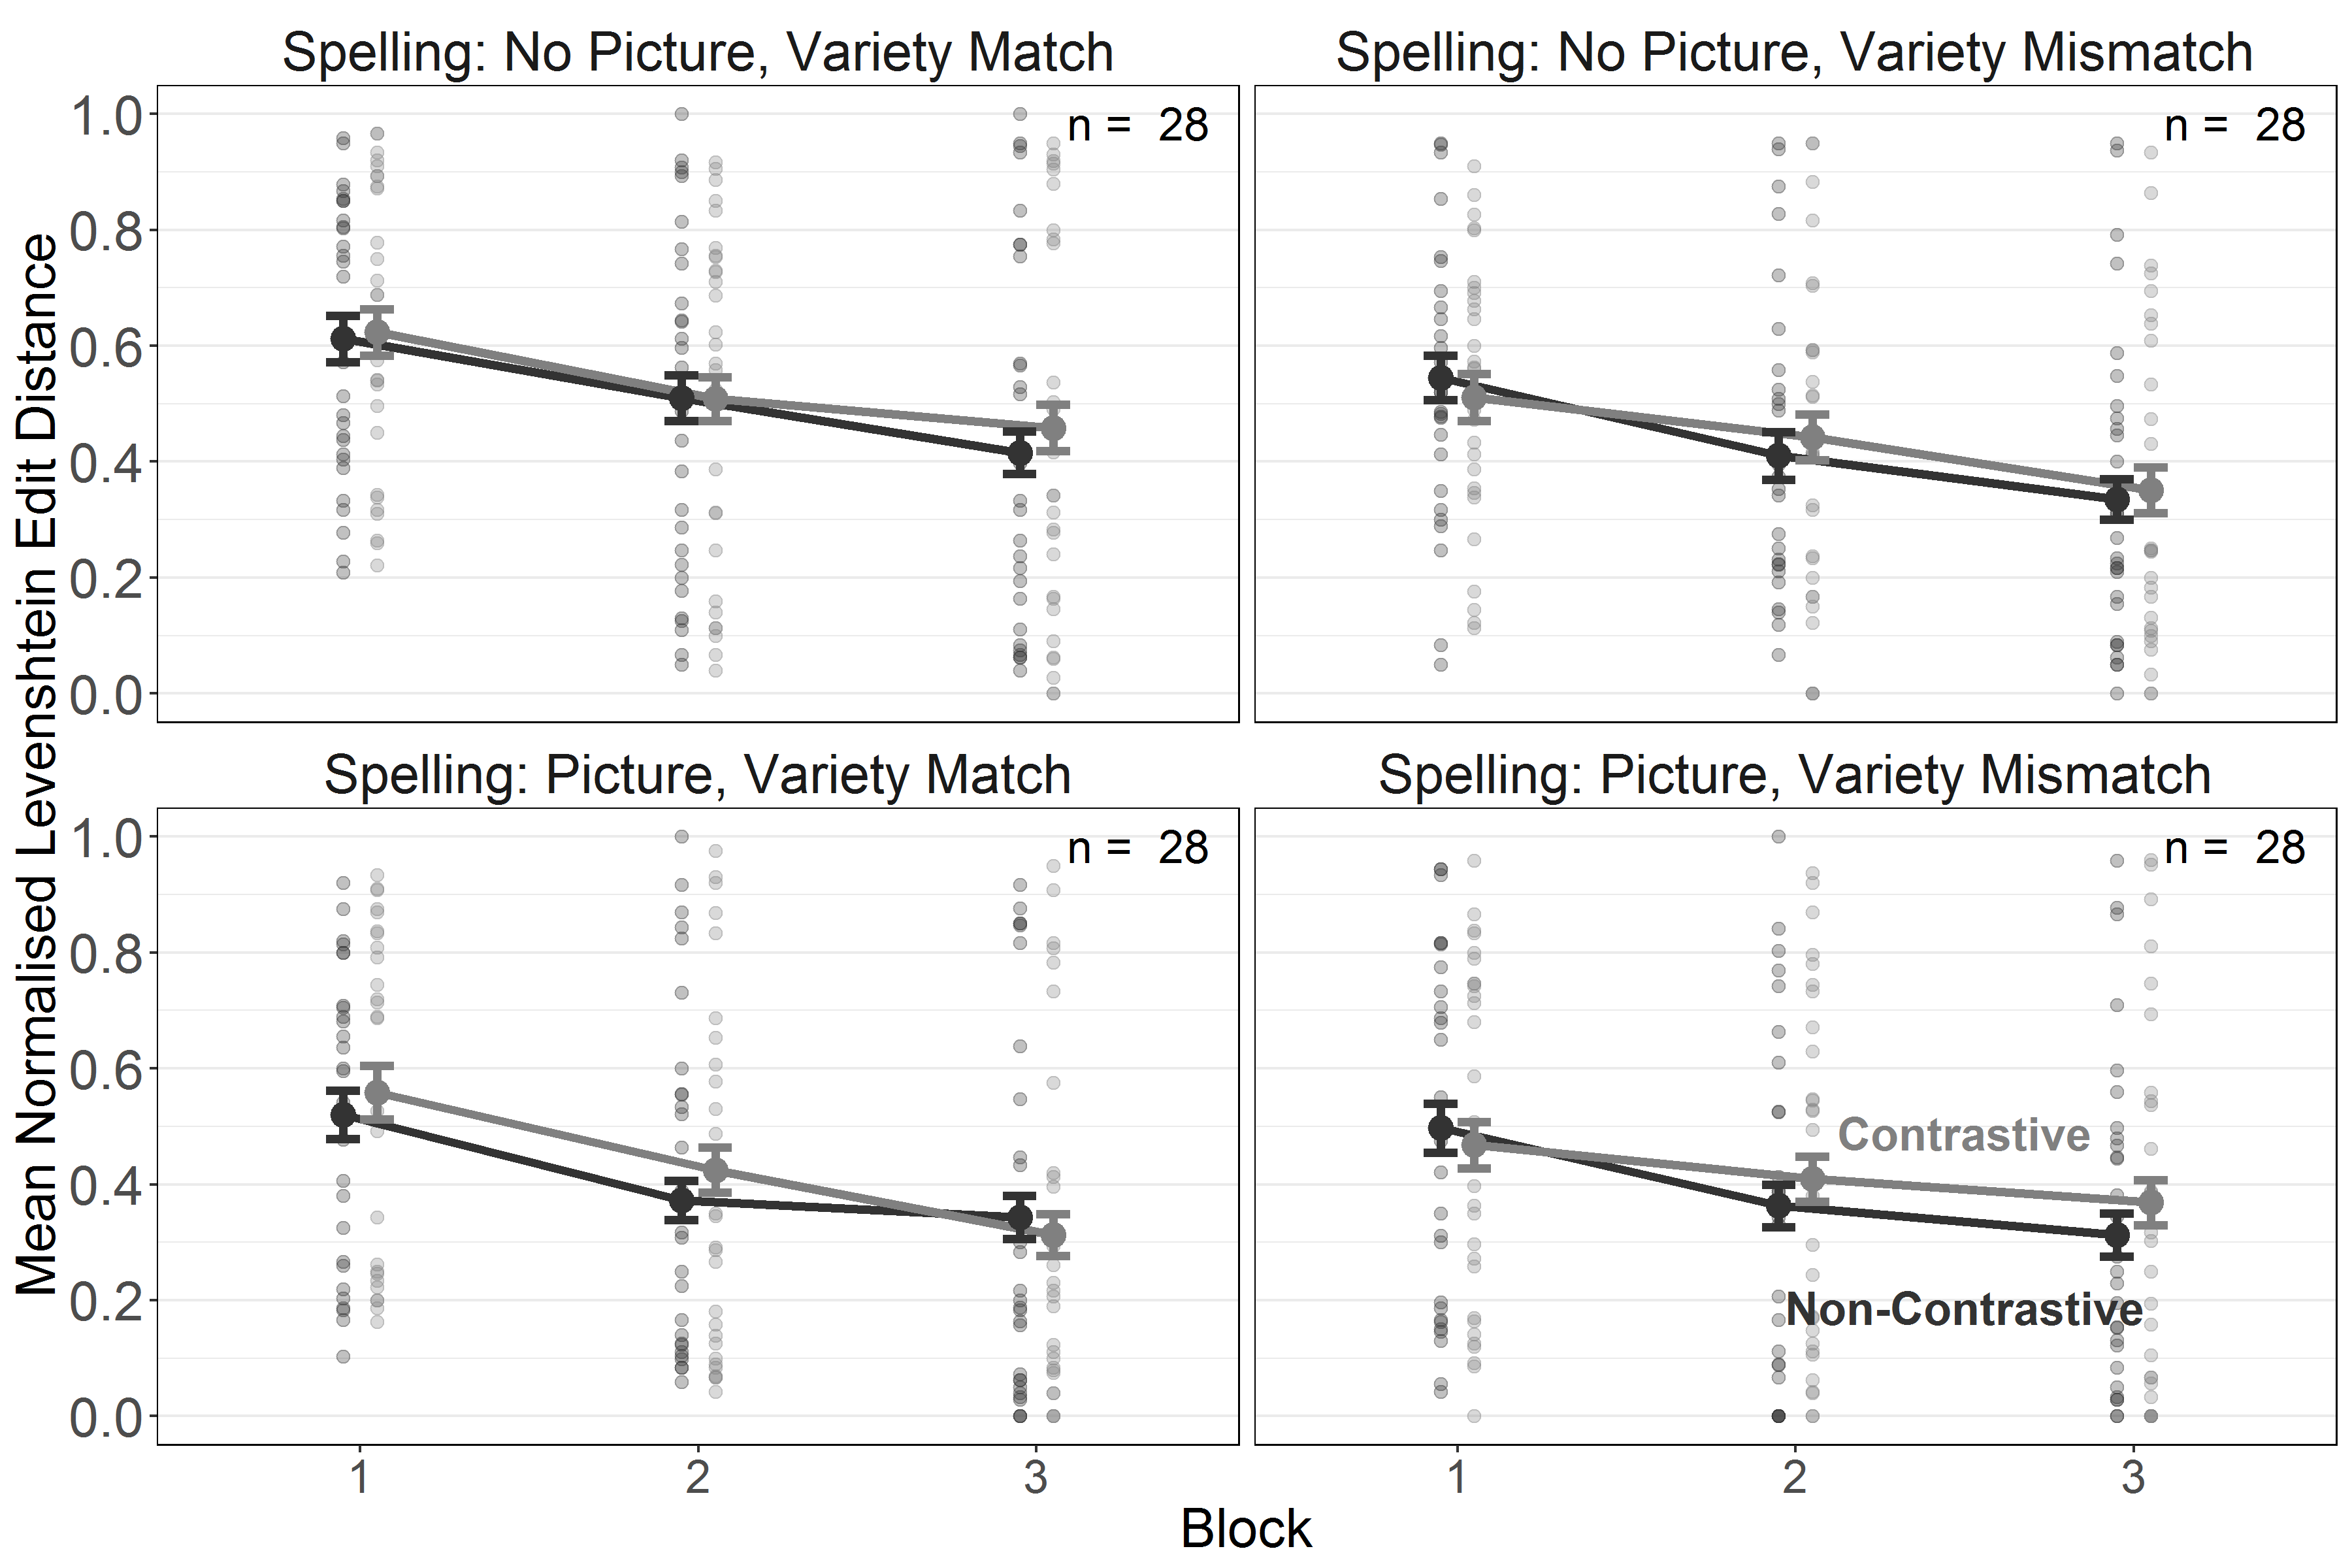
\includegraphics[width=1\linewidth]{C:/Users/g517364/Dropbox/GitHub/levenik/04_figures/output/experiment-1_training_plot_spelling} 

}

\caption{Experiment 2a. Length-normalised Levenshtein Edit Distance for spelling of contrastive and non-contrastive words during 3 training blocks in the variety match and variety mismatch conditions. Error bars indicate $\pm$ 1 $SE$ of the mean.}\label{fig:ex1-train-spelling-plots}
\end{figure}

\paragraph{Testing}\label{testing-1}

Parameter estimates, confidence intervals (for the frequentist analysis)
and credible intervals (for the Bayesian analysis) are presented in
Table~\ref{tab:ex1-test} and depicted in
Figures~\ref{fig:ex1-test-reading-plots} and
\ref{fig:ex1-test-spelling-plots}. The results confirmed the main effect
of task observed during training which showed that performance was
superior for reading compared to spelling. As during training, we found
an effect of Word Type, which is indicative of impaired performance with
contrastive words, in the Variety Mismatch condition but only when
pictures were present. The effect of Word Familiarity was significant in
all conditions except for spelling in the Variety Mismatch condition
with pictures, although Bayesian analyses failed to corroborate it for
spelling in the Variety Match condition without pictures.

\begin{table}[!h]

\caption{\label{tab:ex1-test}Experiment 2a. Parameter estimates for the models fitted to nLEDs from the testing phase. Bayesian analyses report standardised parameter estimates (i.e. the intercept [grand mean] is centred at 0). Values of 0 with a sign indicate the direction of the estimate before rounding.}
\centering
\resizebox{\linewidth}{!}{
\fontsize{8}{10}\selectfont
\begin{tabular}{lrrlrlrrl}
\toprule
\multicolumn{1}{c}{ } & \multicolumn{5}{c}{Frequentist Estimates} & \multicolumn{3}{c}{Bayesian Estimates} \\
\cmidrule(l{3pt}r{3pt}){2-6} \cmidrule(l{3pt}r{3pt}){7-9}
Term & $Est.$ & $SE$ & 95\% Conf. I & $t$ & $p$ & $Est.$ & $SE$ & 95\% Cred. I\\
\midrule
Intercept & 0.52 & 0.04 & [0.44, 0.60] & 12.75 & < .001*** & 0.01 & 0.08 & [-0.15, 0.16]\\
\textbf{Task} & \textbf{-0.04} & \textbf{0.01} & \textbf{[-0.06, -0.03]} & \textbf{-6.72} & \textbf{< .001***} & \textbf{-0.08} & \textbf{0.01} & \textbf{[-0.11, -0.06]}\\
Picture Condition & 0.05 & 0.04 & [-0.03, 0.13] & 1.14 & < .001*** & 0.07 & 0.08 & [-0.09, 0.21]\\
Variety Condition & -0.05 & 0.04 & [-0.13, 0.03] & -1.15 & < .001*** & -0.09 & 0.07 & [-0.24, 0.05]\\
TC $\times$ PC & 0.00 & 0.01 & [-0.01, 0.01] & 0.13 & 1.00 & 0.00 & 0.01 & [-0.02, 0.02]\\
TC $\times$ VC & 0.00 & 0.01 & [-0.02, 0.01] & -0.72 & < .001*** & -0.01 & 0.01 & [-0.03, 0.01]\\
PC $\times$ VC & -0.04 & 0.04 & [-0.12, 0.04] & -1.03 & < .001*** & -0.07 & 0.07 & [-0.21, 0.07]\\
TC $\times$ PC $\times$ VC & 0.00 & 0.01 & [-0.01, 0.02] & 0.76 & < .001*** & 0.01 & 0.01 & [-0.01, 0.03]\\
R, NP, VMis: WT & -0.02 & 0.02 & [-0.06, 0.01] & -1.25 & < .001*** & -0.04 & 0.03 & [-0.11, 0.02]\\
S, NP, VMis: WT & -0.01 & 0.02 & [-0.04, 0.02] & -0.41 & 1.00 & -0.01 & 0.03 & [-0.06, 0.05]\\
\textbf{R, P, VMis: WT} & \textbf{-0.05} & \textbf{0.02} & \textbf{[-0.09, -0.02]} & \textbf{-3.19} & \textbf{< .001***} & \textbf{-0.10} & \textbf{0.03} & \textbf{[-0.16, -0.04]}\\
S, P, VMis: WT & -0.01 & 0.02 & [-0.04, 0.02] & -0.89 & < .001*** & -0.02 & 0.03 & [-0.08, 0.03]\\
R, NP, VMa: WT & -0.02 & 0.02 & [-0.05, 0.01] & -1.10 & < .001*** & -0.03 & 0.03 & [-0.09, 0.03]\\
S, NP, VMa: WT & 0.00 & 0.01 & [-0.03, 0.02] & -0.15 & 1.00 & 0.00 & 0.03 & [-0.05, 0.05]\\
R, P, VMa: WT & 0.00 & 0.02 & [-0.04, 0.03] & -0.17 & 1.00 & 0.00 & 0.03 & [-0.06, 0.06]\\
S, P, VMa: WT & 0.00 & 0.01 & [-0.03, 0.02] & -0.10 & 1.00 & 0.00 & 0.03 & [-0.05, 0.05]\\
\textbf{R, NP, VMis, WF} & \textbf{0.03} & \textbf{0.01} & \textbf{[0.01, 0.06]} & \textbf{2.53} & \textbf{< .001***} & \textbf{0.06} & \textbf{0.02} & \textbf{[0.02, 0.11]}\\
\textbf{S, NP, VMis, WF} & \textbf{0.02} & \textbf{0.01} & \textbf{[0.00, 0.04]} & \textbf{2.21} & \textbf{< .001***} & \textbf{0.04} & \textbf{0.02} & \textbf{[0.01, 0.08]}\\
\textbf{R, P, VMis, WF} & \textbf{0.05} & \textbf{0.01} & \textbf{[0.03, 0.07]} & \textbf{4.07} & \textbf{< .001***} & \textbf{0.09} & \textbf{0.02} & \textbf{[0.05, 0.14]}\\
S, P, VMis, WF & 0.01 & 0.01 & [-0.00, 0.03] & 1.47 & < .001*** & 0.03 & 0.02 & [-0.01, 0.06]\\
\textbf{R, NP, VMa, WF} & \textbf{0.03} & \textbf{0.01} & \textbf{[0.01, 0.05]} & \textbf{2.58} & \textbf{< .001***} & \textbf{0.05} & \textbf{0.02} & \textbf{[0.01, 0.10]}\\
S, NP, VMa, WF & 0.02 & 0.01 & [0.00, 0.03] & 2.03 & < .001*** & 0.03 & 0.02 & [-0.00, 0.07]\\
\textbf{R, P, VMa, WF} & \textbf{0.03} & \textbf{0.01} & \textbf{[0.00, 0.05]} & \textbf{2.35} & \textbf{< .001***} & \textbf{0.05} & \textbf{0.02} & \textbf{[0.01, 0.10]}\\
\textbf{S, P, VMa, WF} & \textbf{0.02} & \textbf{0.01} & \textbf{[0.00, 0.03]} & \textbf{2.48} & \textbf{< .001***} & \textbf{0.04} & \textbf{0.02} & \textbf{[0.00, 0.07]}\\
\bottomrule
\multicolumn{9}{l}{Variety Condition (VC) = variety match vs. variety mismatch (VMa vs. VMi),}\\
\multicolumn{9}{l}{Picture Condition (PC) = picture vs. no picture (P vs. NP), Task Condition (TC) = reading vs. spelling (R vs. S),}\\
\multicolumn{9}{l}{Word Type (WT) = contrastive vs. non-contrastive, Word Familiarity (WF) = familiar vs. unfamiliar (novel)}\\
\end{tabular}}
\end{table}

\begin{figure}[htb]

{\centering 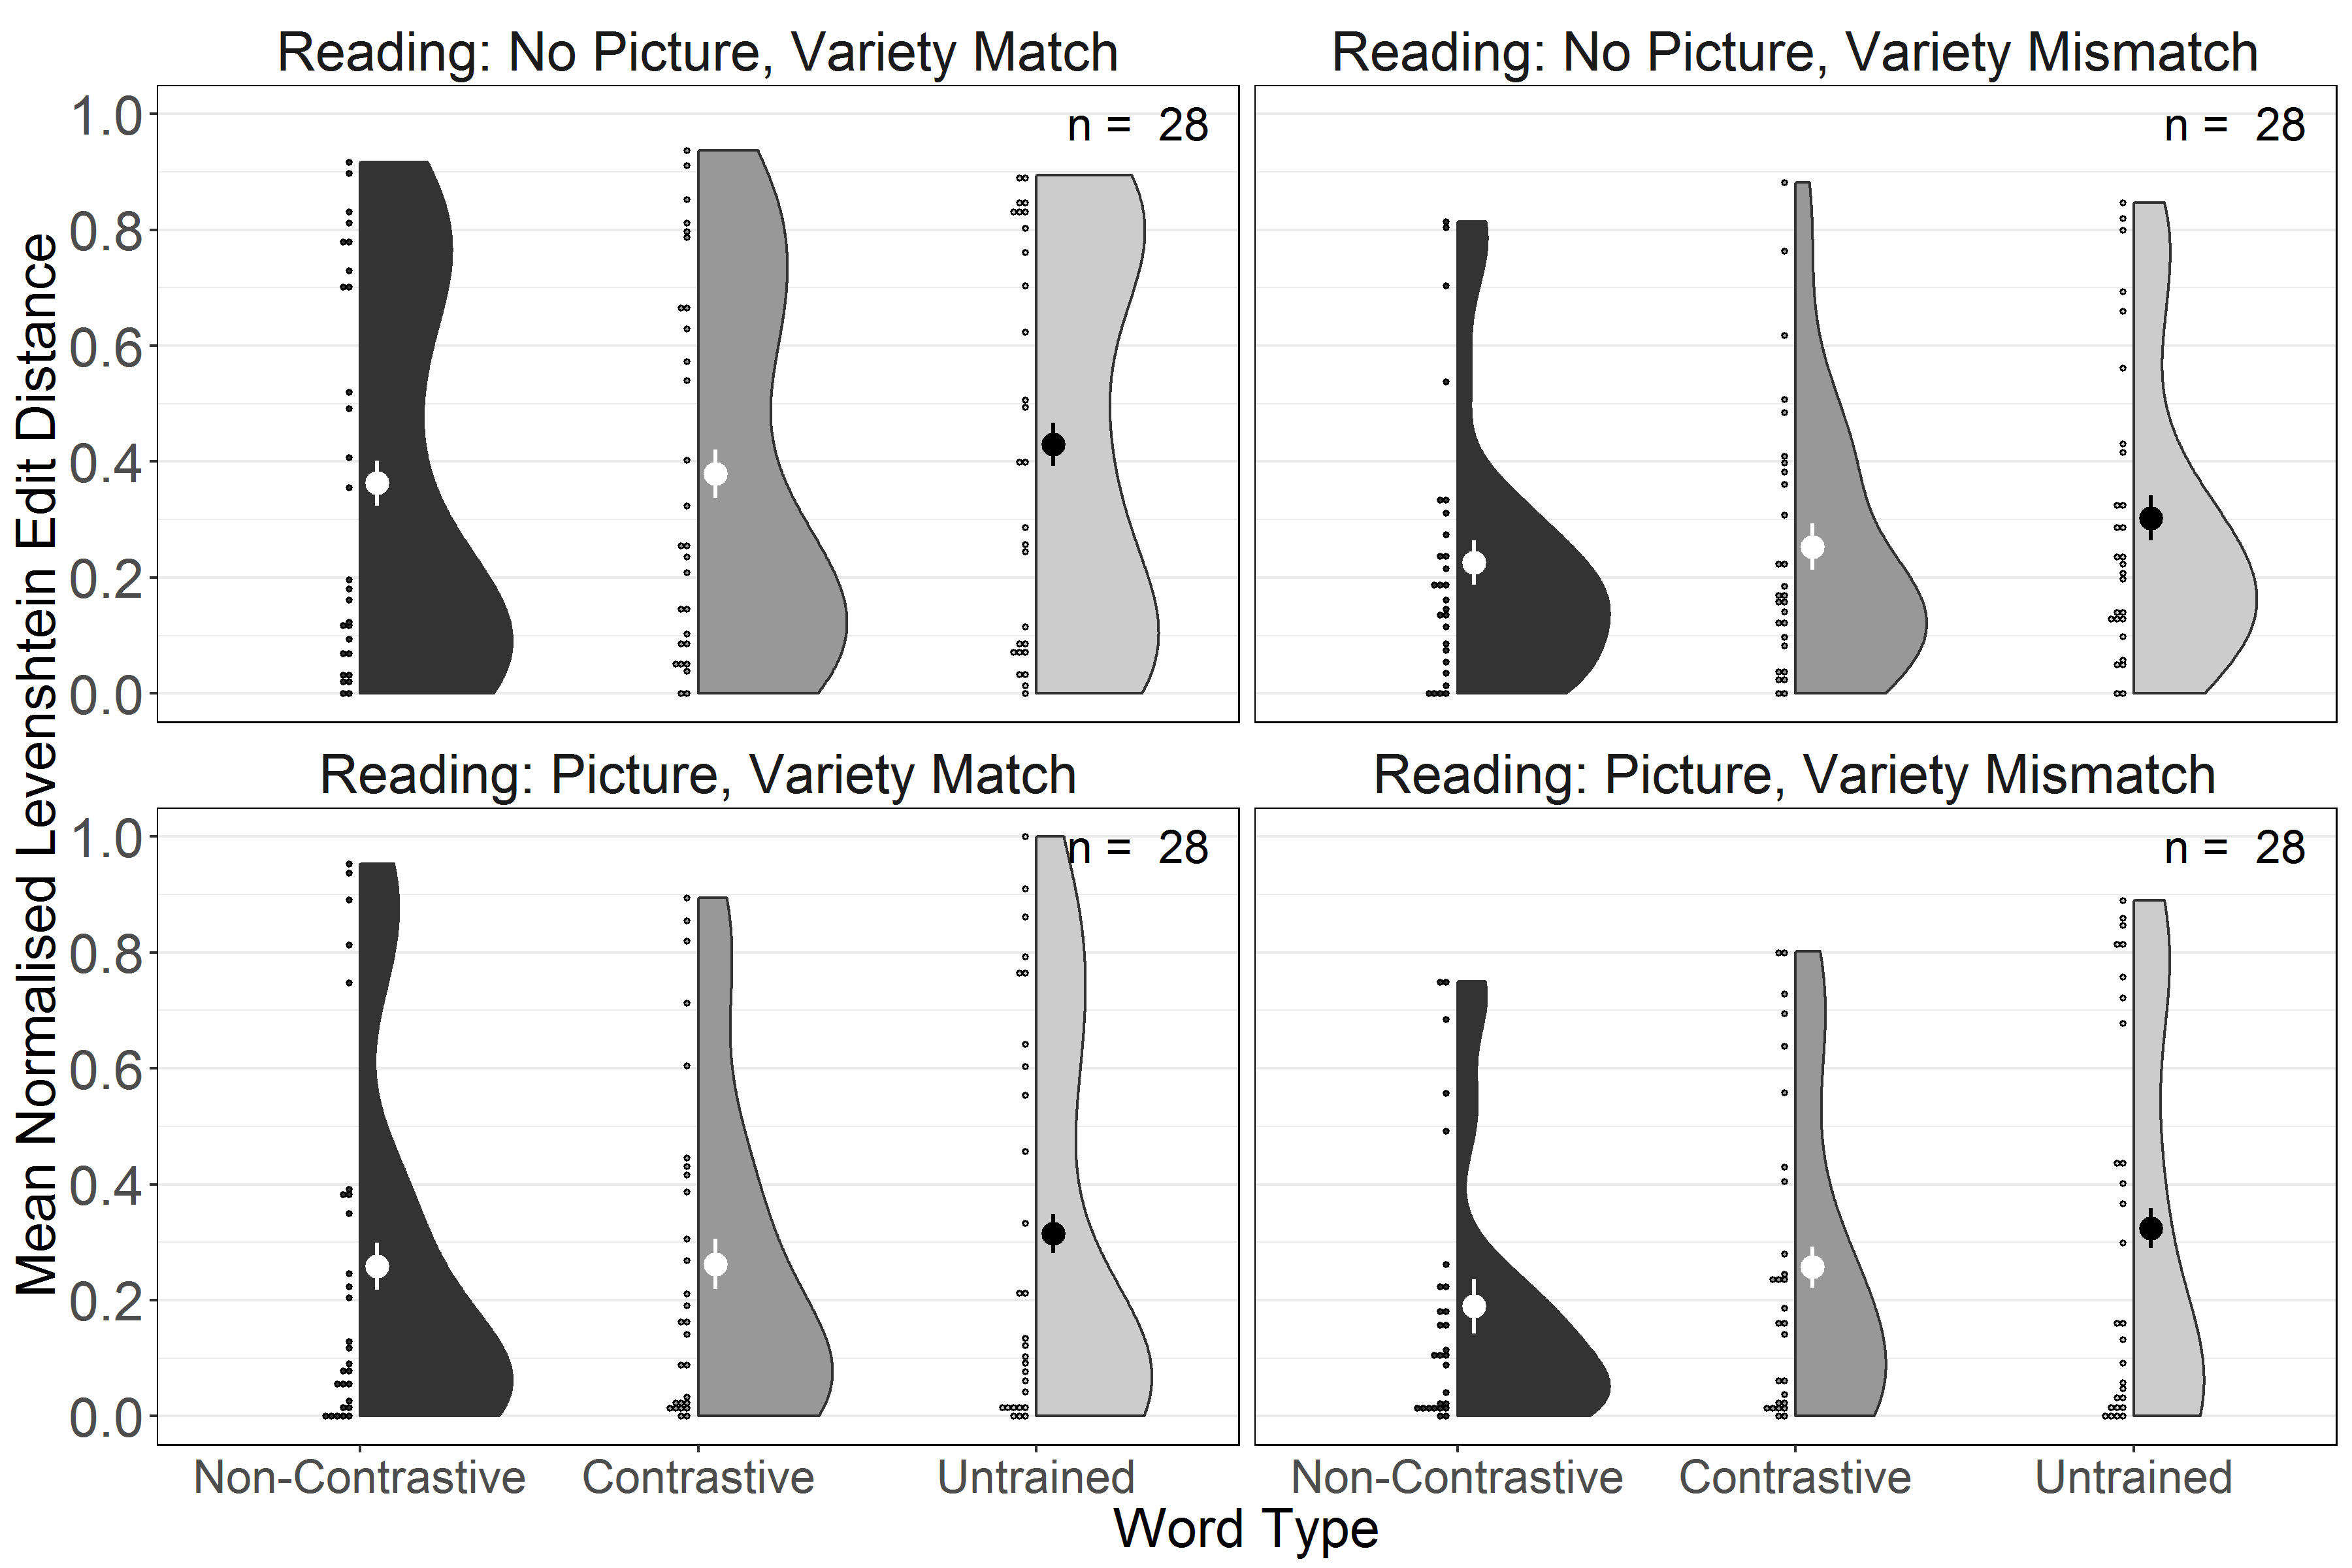
\includegraphics[width=1\linewidth]{C:/Users/g517364/Dropbox/GitHub/levenik/04_figures/output/experiment-1_testing_plot_reading} 

}

\caption{Experiment 2a. Length-normalised Levenshtein Edit Distance for testing reading performance for trained non-contrastive, trained contrastive and untrained words in the variety match and variety mismatch conditions. Large dots and whiskers indicate means and $\pm$ 1 $SE$ of the mean.}\label{fig:ex1-test-reading-plots}
\end{figure}

\begin{figure}[htb]

{\centering 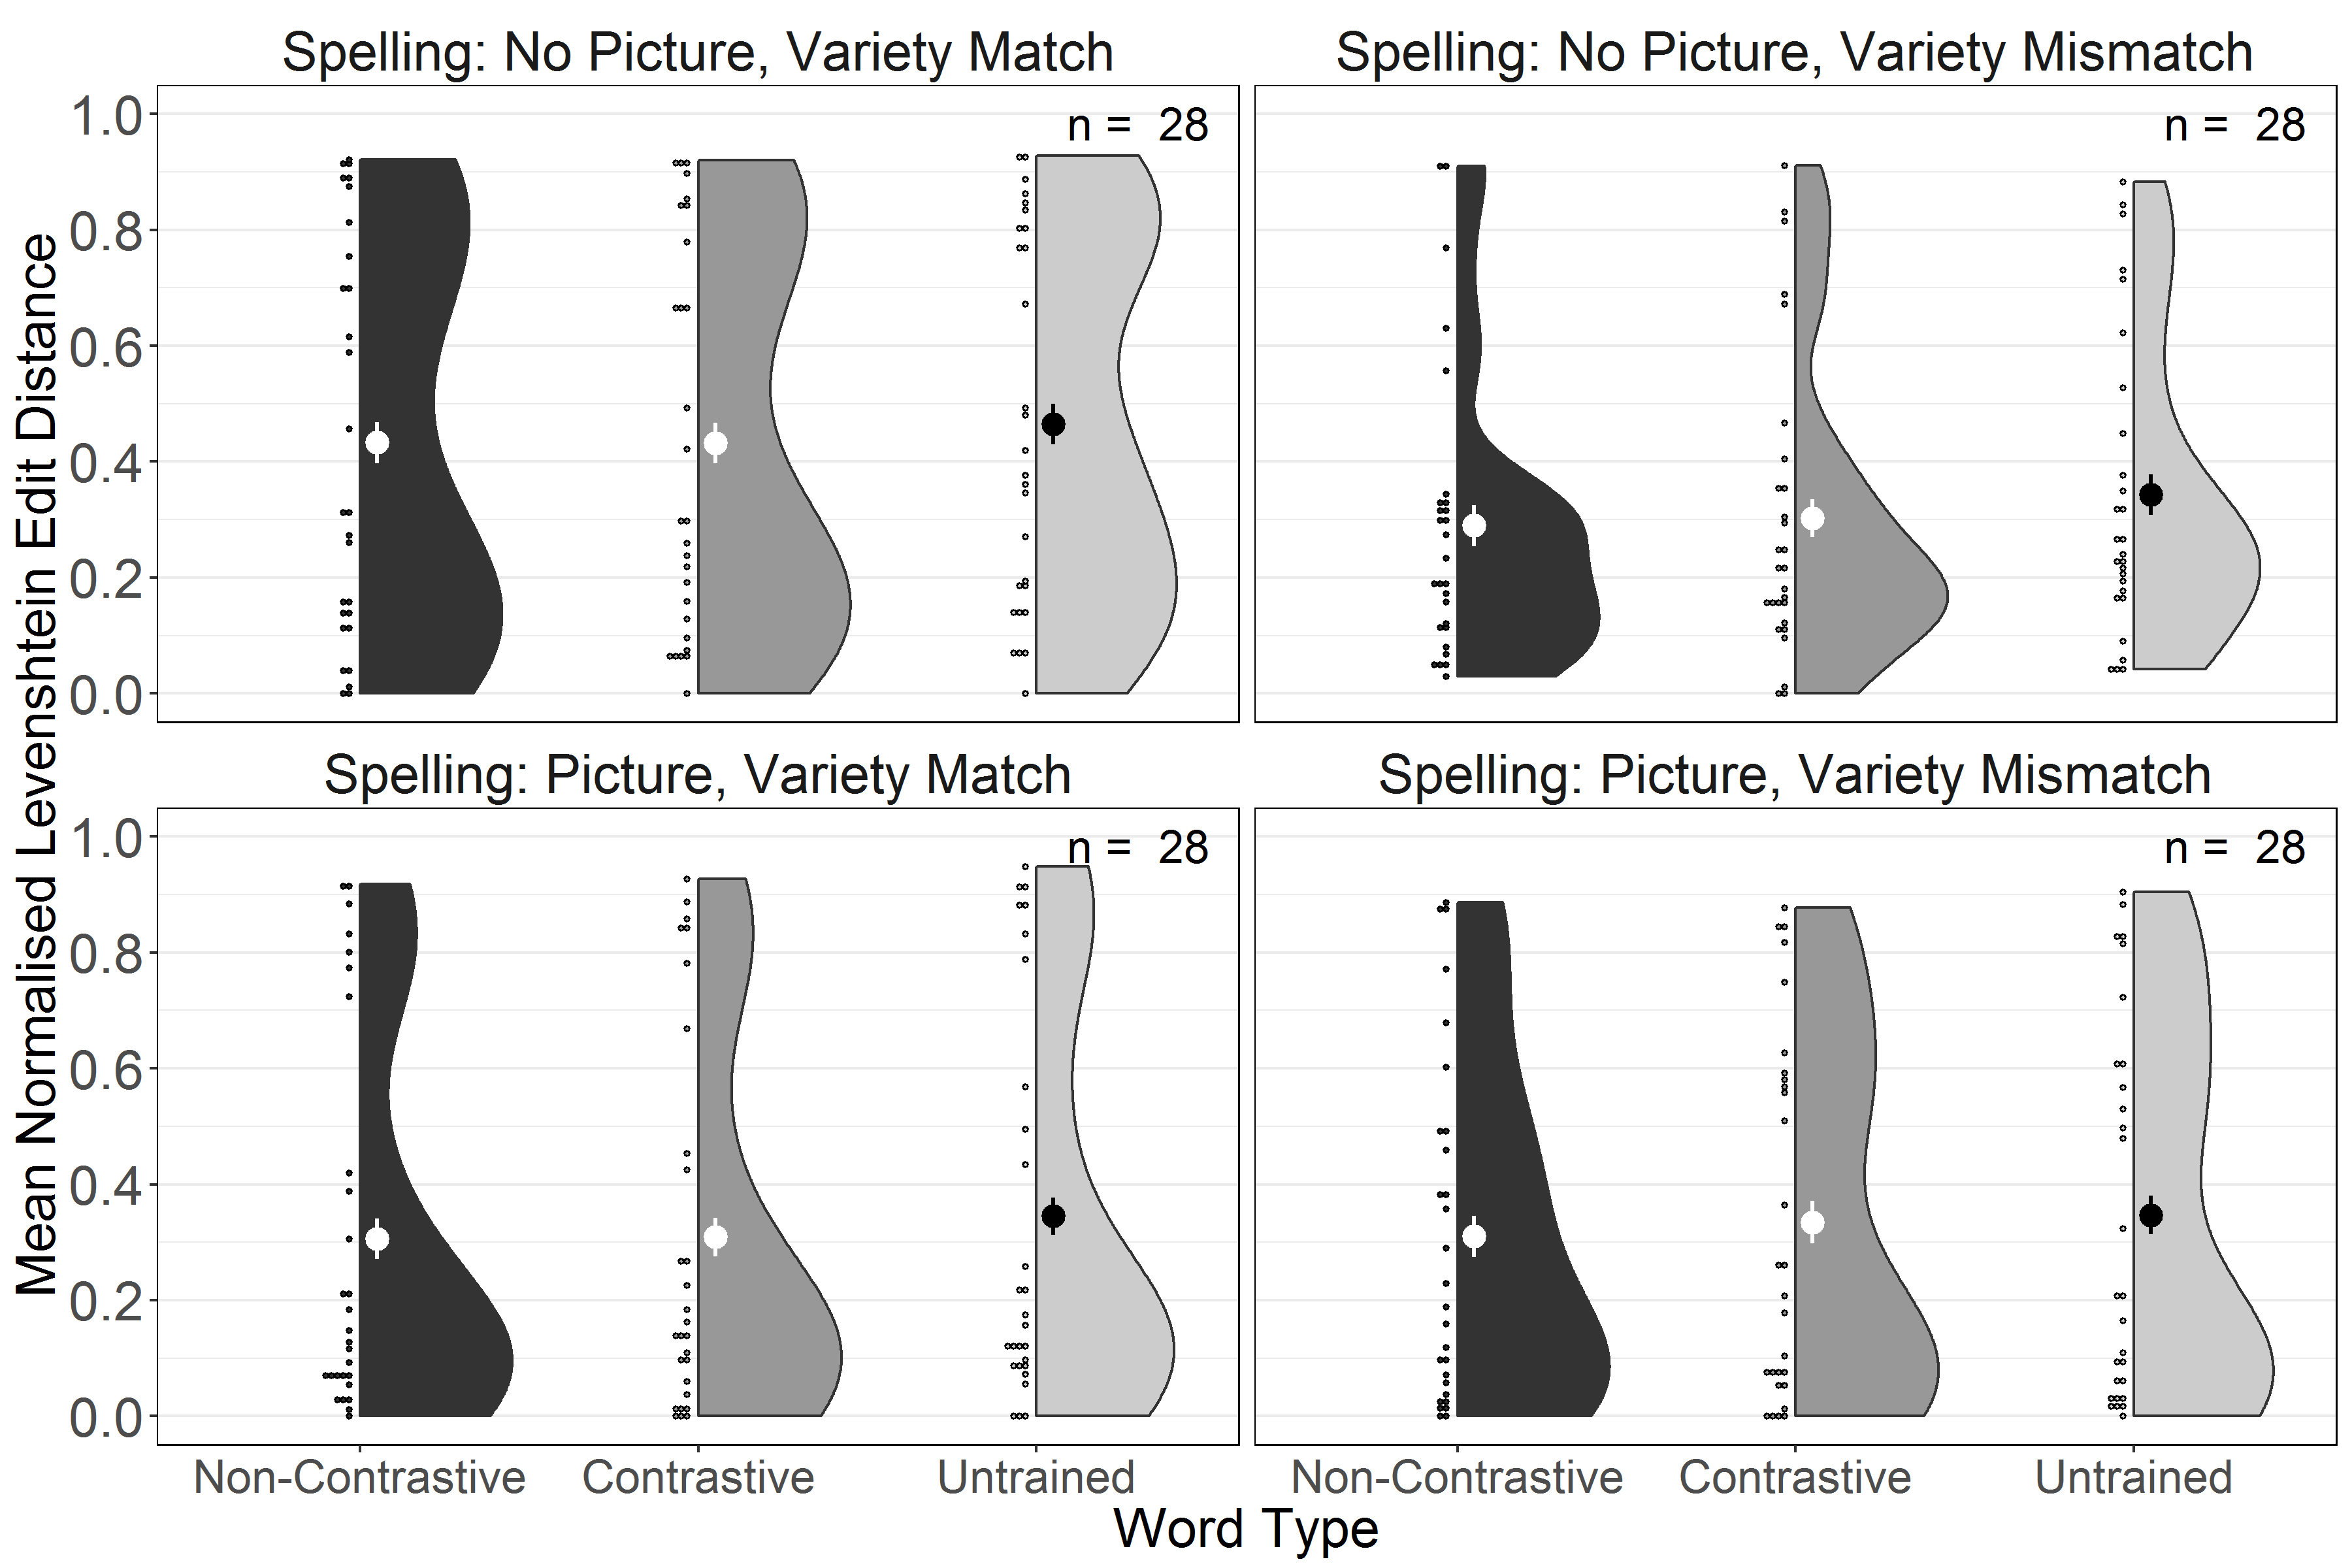
\includegraphics[width=1\linewidth]{C:/Users/g517364/Dropbox/GitHub/levenik/04_figures/output/experiment-1_testing_plot_spelling} 

}

\caption{Experiment 2a. Length-normalised Levenshtein Edit Distance for testing spelling performance for trained non-contrastive, trained contrastive and untrained words in the variety match and variety mismatch conditions. Large dots and whiskers indicate means and $\pm$ 1 $SE$ of the mean.}\label{fig:ex1-test-spelling-plots}
\end{figure}

As in Experiment 1, we performed a planned direct comparison of
performance on untrained words between all Variety Match and Variety
Mismatch conditions. The model included fixed effects and interactions
between the sum-coded Task Condition, Picture Condition and Language
Variety. We used the same criteria as in our main models for determining
the random effects structure of the model. Here, this took the form of
zero-correlation random intercepts and slopes of Task Condition, Picture
Condition and Language Variety and their interaction by items, and
random intercepts by subjects. As in Experiment 1, the effect of Variety
provided no evidence for a detrimental effect of a variety mismatch on
reading and spelling of untrained words (frequentist estimate:
\(\hat{\beta}\) = -0.04{[}-0.12, 0.04{]}, \emph{t} = -0.93, \emph{p} =
\textless{} .001***; Bayesian Estimate: \(\hat{\beta}\) = -0.06{[}-0.21,
0.07{]}).

\subsection{Discussion}\label{discussion-1}

When spelling was introduced to the literacy training in a transparent
artificial orthography, we observed that a contrastive deficit emerged
in reading when participants were exposed to variety mismatch, which
persisted into the testing session when pictures provided an opportunity
to establish semantic representations. This contrastive deficit in
reading replicates the contrastive deficit found by Brown et al. (2015)
for both children and a neural network exposed to both AAE and MAE but
unlike in that study, it was more persistent when participants were able
to establish semantic representations. It is noteworthy that no
contrastive deficit emerged for spelling. This is because no competing
orthographic representations for words in the exposure variety (i.e.~the
\enquote{dialect}) exist and learners are likely to adopt a strategy of
sequentially converting phonemes into graphemes.

We had expected that introducing spelling would also facilitate reliance
on sequential decoding using grapheme-phoneme conversion during reading.
Had participants adopted such a strategy exclusively, we should not have
observed any effect of word familiary manifesting itself in impaired
performance for untrained words. Yet the effect of word familiarity was
significant in all reading conditions and even some of the spelling
conditions suggesting that despite the transparent orthography, which
encourages systematic mapping of graphemes onto phoneme and vice versa,
participant still to some extent attempted to access phonological (in
the case of reading) and even orthographic (in the case of spelling)
representations more directly. Specifically, their emerging word
knowledge may have resulted in a reading strategy that involved decoding
just enough graphemes to be able to access the memorised word form so
that knowledge of word forms benefitted trained but not untrained items.
The familiarity effect in spelling is a bit more puzzling but may
reflect emergence of representations of the overall graphemic Gestalt or
even the motor routine required to type a word which may have
facilitated spelling. Most importantly for the main question of the
study, the lack of evidence for a difference between the variety match
and mismatch conditions in reading and spelling of untrained words
suggests that concurrent exposure to another variety did not appear to
have any further detrimental effect on whatever limited amount of
decoding skills participants had acquired.

\section{Experiment 2b: Opaque
Orthography}\label{experiment-2b-opaque-orthography}

\subsection{Method}\label{method-2}

\subsubsection{Participants}\label{participants-2}

One hundred and twelve participants (aged aged 20--68, \emph{M} = 33.29,
\emph{SD} = 9.75) were recruited from Amazon's Mechanical Turk and took
part in the study for \$7.50. All participants reported proficiency in
English (1-7 Likert scale: \emph{M} = 4.77, \emph{SD} = 0.57). Another 3
participants were tested and excluded based on the exclusion criteria
described for Experiment 1.

\subsubsection{Materials}\label{materials-2}

Graphemes, words and pictures were identical to the previous two
experiments. We used the same opaque orthography as in Experiment 1.

\subsubsection{Procedure}\label{procedure-2}

The procedure was identical to Experiment 2a. The mean completion time
was 81.38 minutes (\emph{SD} = 42.82).

\subsection{Results}\label{results-2}

\subsubsection{Coding}\label{coding-2}

We used the same coding scheme for reading responses as in the previous
experiments. The ICC between coders was F(16124.00, 15907.98) = 63.01,
\(p\) \textless{} .001, ICC = 0.97 {[}95\% CI = 0.97; 0.97{]}. The 95\%
confidence interval around the parameter estimate indicates that the ICC
falls above the bound of .90, which suggests excellent reliability
across raters (see Koo \& Li, 2016).

\subsubsection{Model Fitting}\label{model-fitting-2}

Frequentist and Bayesian analyses were conducted in the same way as for
Experiment 2b. However, due to differences in convergence for the
frequentist analyses across the two experiments, Experiment 2b had some
minor differences in the random effects structure of frequentist models
when compared to Experiment 2a. For the training phase, the maximal
converging random effects structure included correlations between all
by-participant terms. For the testing phase, correlations were
suppressed between all random effects terms.

\paragraph{Training}\label{training-2}

Parameter estimates, confidence intervals (for the frequentist analysis)
and credible intervals (for the Bayesian analysis) are presented in
Table~\ref{tab:ex2-train} and depicted in
Figures~\ref{fig:ex2-train-reading-plots} and
\ref{fig:ex2-train-spelling-plots}.

\begin{table}[!h]

\caption{\label{tab:ex2-train}Experiment 2b. Parameter estimates for the models fitted to nLEDs from the training phase. Bayesian analyses report standardised parameter estimates (i.e. the intercept [grand mean] is centred at 0). Values of 0 with a sign indicate the direction of the estimate before rounding.}
\centering
\resizebox{\linewidth}{!}{
\fontsize{8}{10}\selectfont
\begin{tabular}{lrrlrlrrl}
\toprule
\multicolumn{1}{c}{ } & \multicolumn{5}{c}{Frequentist Estimates} & \multicolumn{3}{c}{Bayesian Estimates} \\
\cmidrule(l{3pt}r{3pt}){2-6} \cmidrule(l{3pt}r{3pt}){7-9}
Term & $Est.$ & $SE$ & 95\% Conf. I & $t$ & $p$ & $Est.$ & $SE$ & 95\% Cred. I\\
\midrule
Intercept & 0.80 & 0.03 & [0.74, 0.87] & 24.01 & < .001*** & 0.03 & 0.07 & [-0.11, 0.17]\\
\textbf{Block} & \textbf{-6.44} & \textbf{0.68} & \textbf{[-7.78, -5.10]} & \textbf{-9.42} & \textbf{< .001***} & \textbf{-0.28} & \textbf{0.03} & \textbf{[-0.34, -0.22]}\\
\textbf{Task} & \textbf{-0.03} & \textbf{0.01} & \textbf{[-0.05, -0.02]} & \textbf{-4.19} & \textbf{< .001***} & \textbf{-0.07} & \textbf{0.02} & \textbf{[-0.11, -0.04]}\\
Picture Condition & -0.01 & 0.03 & [-0.07, 0.05] & -0.18 & 1.00 & -0.01 & 0.06 & [-0.13, 0.09]\\
Variety Condition & -0.04 & 0.03 & [-0.10, 0.02] & -1.27 & < .001*** & -0.07 & 0.06 & [-0.20, 0.06]\\
B $\times$ TC & -0.28 & 0.39 & [-1.05, 0.50] & -0.70 & < .001*** & -0.01 & 0.02 & [-0.04, 0.02]\\
B $\times$ PC & -0.03 & 0.68 & [-1.37, 1.31] & -0.04 & 1.00 & 0.00 & 0.03 & [-0.06, 0.06]\\
\textbf{TC $\times$ PC} & \textbf{0.02} & \textbf{0.01} & \textbf{[0.01, 0.04]} & \textbf{2.87} & \textbf{< .001***} & \textbf{0.05} & \textbf{0.02} & \textbf{[0.01, 0.08]}\\
B $\times$ VC & -0.92 & 0.68 & [-2.26, 0.42] & -1.35 & < .001*** & -0.04 & 0.03 & [-0.10, 0.02]\\
TC $\times$ VC & 0.00 & 0.01 & [-0.01, 0.02] & 0.22 & 1.00 & 0.00 & 0.02 & [-0.03, 0.04]\\
PC $\times$ VC & 0.01 & 0.03 & [-0.05, 0.07] & 0.45 & 1.00 & 0.02 & 0.06 & [-0.10, 0.14]\\
B $\times$ TC $\times$ PC & 0.66 & 0.39 & [-0.11, 1.43] & 1.67 & < .001*** & 0.03 & 0.02 & [-0.00, 0.06]\\
B $\times$ TC $\times$ VC & -0.58 & 0.39 & [-1.35, 0.20] & -1.46 & < .001*** & -0.03 & 0.02 & [-0.06, 0.01]\\
B $\times$ PC $\times$ VC & 0.40 & 0.68 & [-0.94, 1.73] & 0.58 & 1.00 & 0.02 & 0.03 & [-0.04, 0.07]\\
TC $\times$ PC $\times$ VC & 0.01 & 0.01 & [-0.01, 0.02] & 1.06 & < .001*** & 0.02 & 0.02 & [-0.02, 0.05]\\
B $\times$ TC $\times$ PC $\times$ VC & -0.16 & 0.39 & [-0.93, 0.61] & -0.40 & 1.00 & -0.01 & 0.02 & [-0.04, 0.03]\\
R, NP, VMis: WT & -0.01 & 0.02 & [-0.05, 0.03] & -0.51 & 1.00 & -0.02 & 0.04 & [-0.09, 0.06]\\
S, NP, VMis: WT & -0.01 & 0.02 & [-0.05, 0.02] & -0.71 & < .001*** & -0.02 & 0.04 & [-0.10, 0.05]\\
R, P, VMis: WT & -0.01 & 0.02 & [-0.05, 0.03] & -0.45 & 1.00 & -0.02 & 0.04 & [-0.09, 0.06]\\
S, P, VMis: WT & 0.01 & 0.02 & [-0.02, 0.05] & 0.80 & < .001*** & 0.03 & 0.04 & [-0.04, 0.10]\\
R, NP, VMa: WT & 0.00 & 0.02 & [-0.03, 0.04] & 0.18 & 1.00 & 0.01 & 0.04 & [-0.07, 0.08]\\
S, NP, VMa: WT & -0.02 & 0.02 & [-0.05, 0.02] & -0.87 & < .001*** & -0.03 & 0.04 & [-0.10, 0.04]\\
R, P, VMa: WT & -0.02 & 0.02 & [-0.06, 0.02] & -1.07 & < .001*** & -0.04 & 0.04 & [-0.11, 0.03]\\
S, P, VMa: WT & -0.01 & 0.02 & [-0.05, 0.02] & -0.81 & < .001*** & -0.03 & 0.04 & [-0.10, 0.05]\\
B, R, NP, VMis: WT & -0.14 & 1.01 & [-2.11, 1.84] & -0.14 & 1.00 & -0.01 & 0.04 & [-0.09, 0.08]\\
B, S, NP, VMis: WT & 0.48 & 1.02 & [-1.52, 2.48] & 0.47 & 1.00 & 0.02 & 0.04 & [-0.06, 0.11]\\
B, R, P, VMis: WT & 0.29 & 1.00 & [-1.68, 2.25] & 0.29 & 1.00 & 0.01 & 0.04 & [-0.07, 0.10]\\
B, S, P, VMis: WT & -0.05 & 1.02 & [-2.04, 1.94] & -0.05 & 1.00 & 0.00 & 0.04 & [-0.08, 0.08]\\
B, R, NP, VMa: WT & 1.44 & 1.00 & [-0.52, 3.40] & 1.44 & < .001*** & 0.06 & 0.04 & [-0.02, 0.15]\\
B, S, NP, VMa: WT & 0.64 & 1.01 & [-1.34, 2.63] & 0.63 & 1.00 & 0.03 & 0.04 & [-0.06, 0.11]\\
B, R, P, VMa: WT & 0.90 & 1.01 & [-1.08, 2.89] & 0.89 & < .001*** & 0.04 & 0.04 & [-0.05, 0.12]\\
B, S, P, VMa: WT & 0.50 & 1.02 & [-1.50, 2.51] & 0.49 & 1.00 & 0.02 & 0.04 & [-0.06, 0.10]\\
\bottomrule
\multicolumn{9}{l}{Block (B) = 1-3, Variety Condition (VC) = variety match vs. variety mismatch (VMa vs. VMi),}\\
\multicolumn{9}{l}{Picture Condition (PC) = picture vs. no picture (P vs. NP), Task Condition (TC) = reading vs. spelling (R vs. S),}\\
\multicolumn{9}{l}{Word Type (WT) = contrastive vs. non-contrastive}\\
\end{tabular}}
\end{table}

As in Experiment 2a, the main effect of Block indicated improvement in
performance over the course of training and the main effect of task
confirmed that learning to spell was more difficult than learning to
read. The only other significant effect was an interaction between task
and picture condition. Pairwise contrasts based on the estimated
marginal means of the training model were calculated using the
\emph{emmeans} R-package (Lenth, 2019), using Holm's sequential
Bonferroni correction. These contrasts indicate that reading performance
was better than writing performance in the picture condition only
(Picture, Reading - Writing: \(\Delta{M}\) = -0.12{[}-0.18, -0.05{]},
\emph{t} = -5.02, \emph{p} = \textless{} .001). All other contrasts were
non-significant (\emph{p} \textgreater{} .05). Unlike Experiment 1, we
did not find any evidence for a contrastive deficit.

\begin{figure}[htb]

{\centering 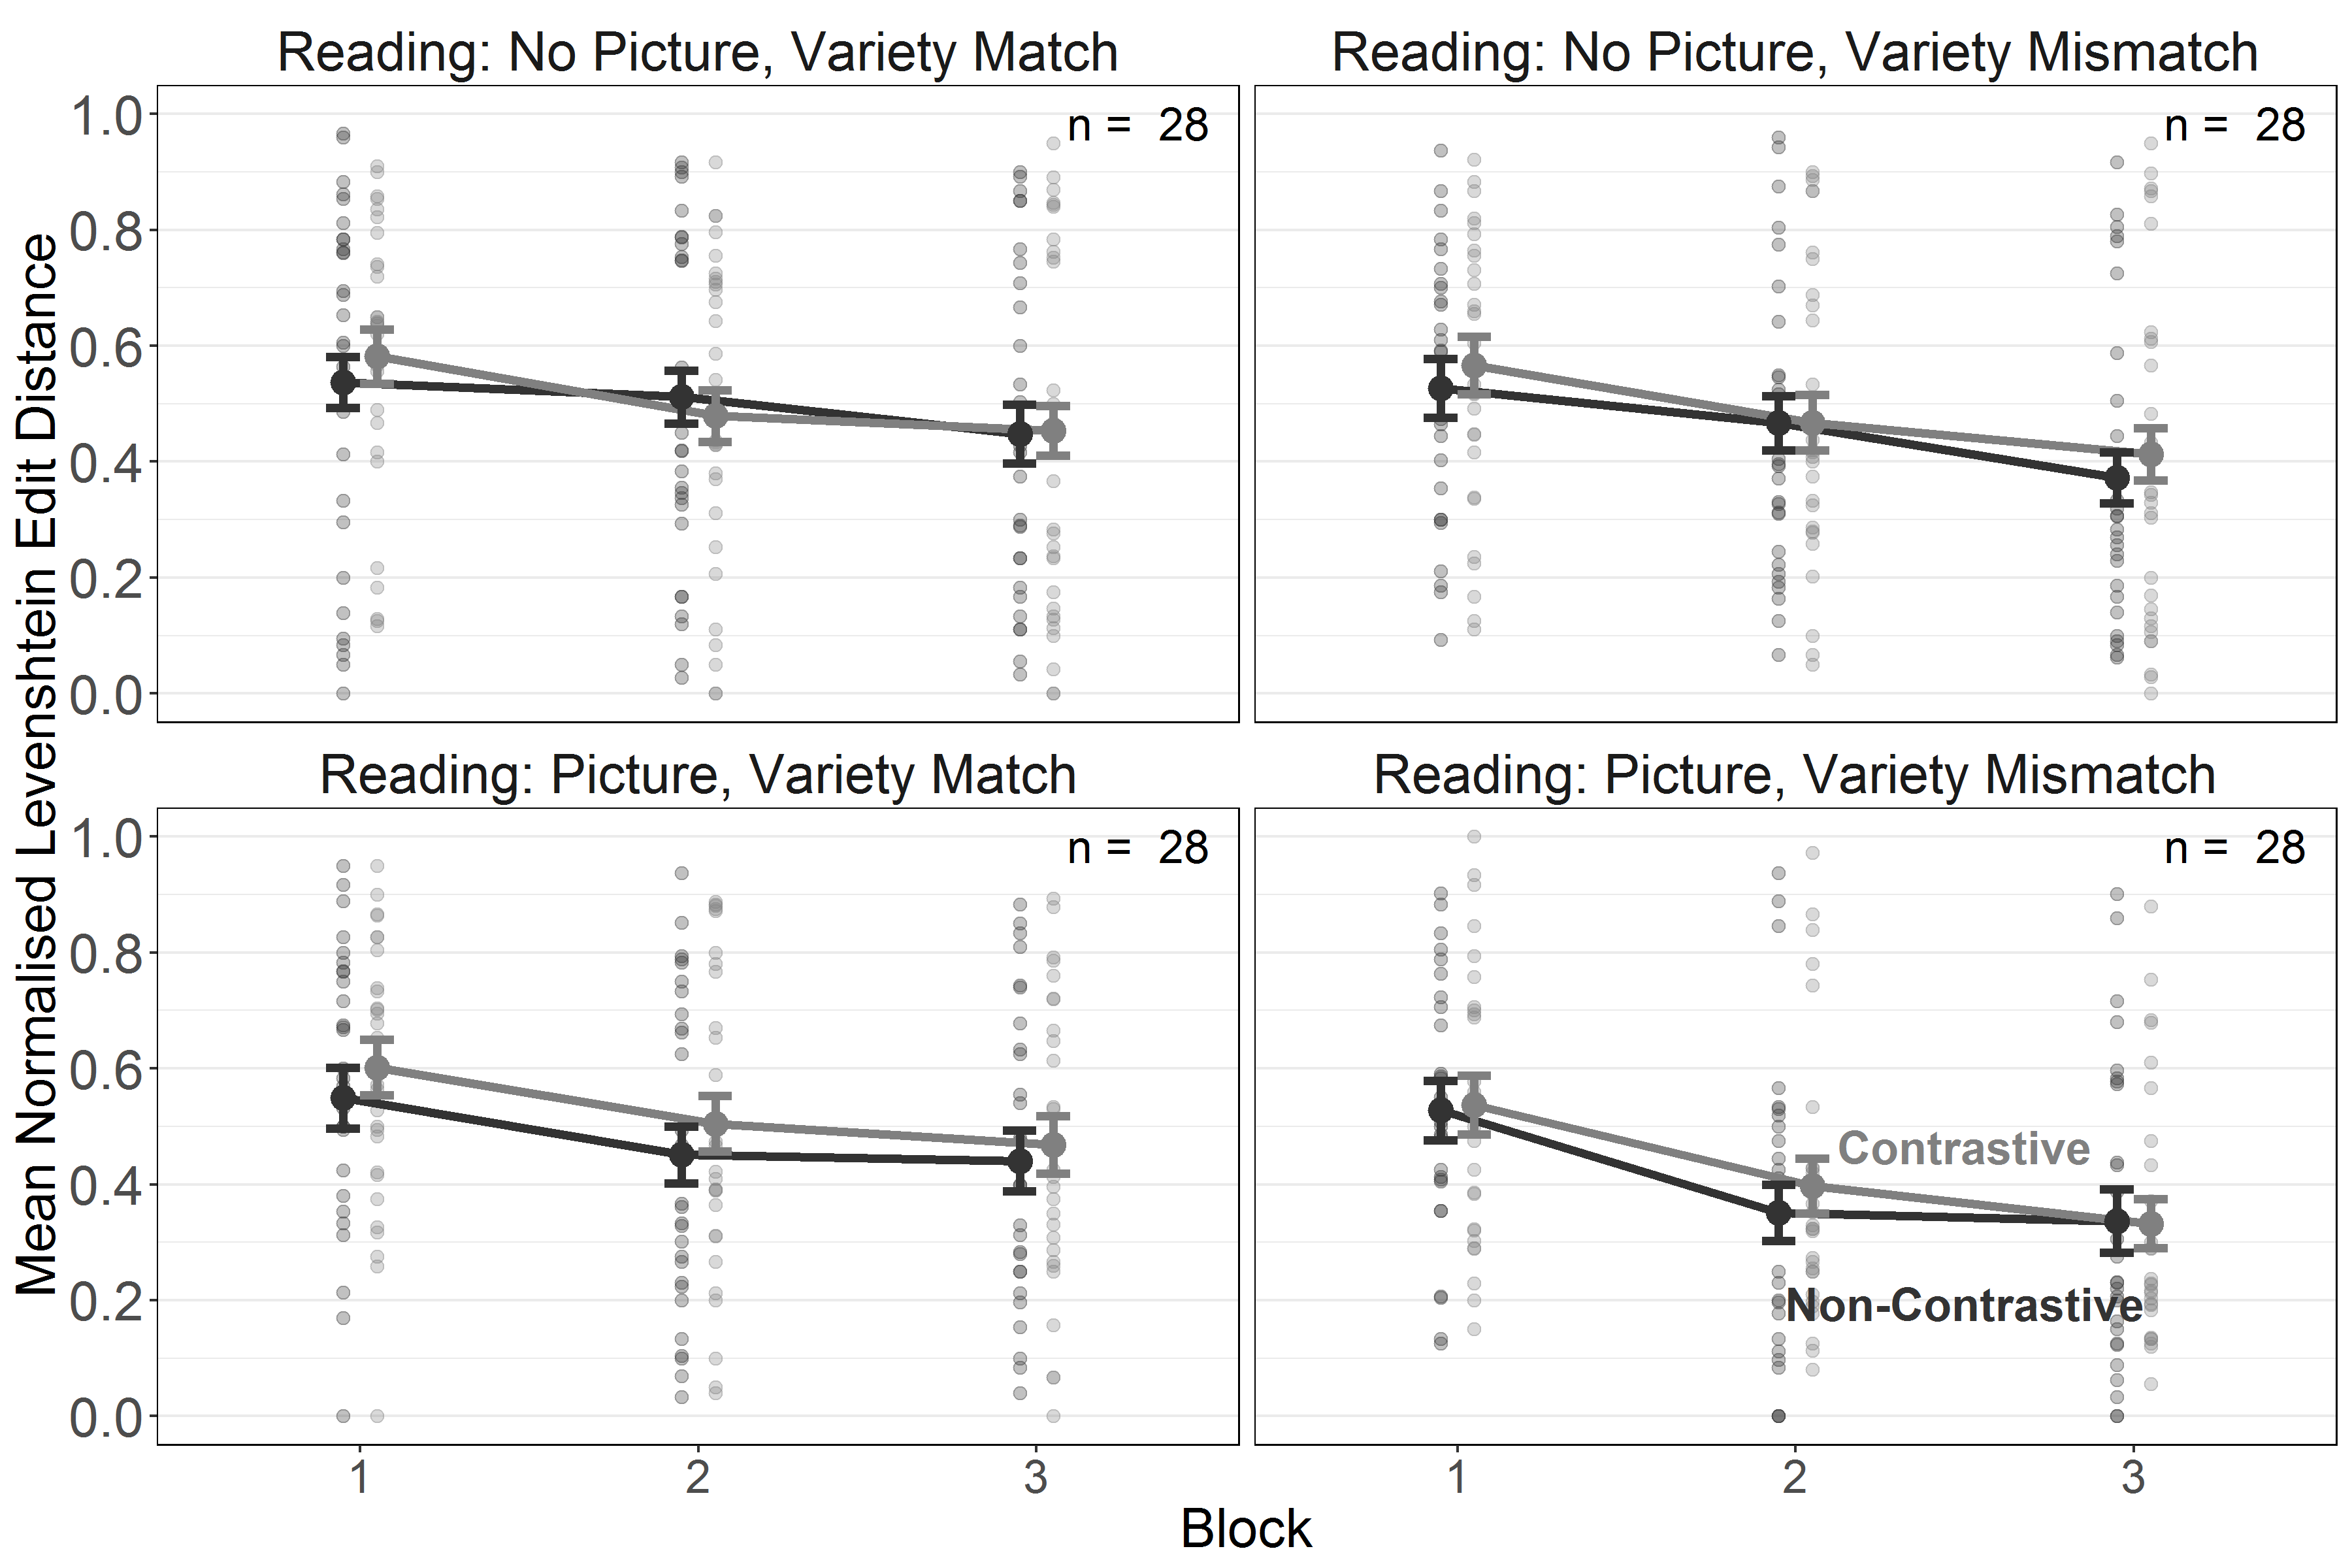
\includegraphics[width=1\linewidth]{C:/Users/g517364/Dropbox/GitHub/levenik/04_figures/output/experiment-2_training_plot_reading} 

}

\caption{Experiment 2b. Length-normalised Levenshtein Edit Distance for reading of contrastive and non-contrastive words during 3 training blocks in the variety match and variety mismatch conditions. Error bars indicate $\pm$ 1 $SE$ of the mean.}\label{fig:ex2-train-reading-plots}
\end{figure}

\begin{figure}[htb]

{\centering 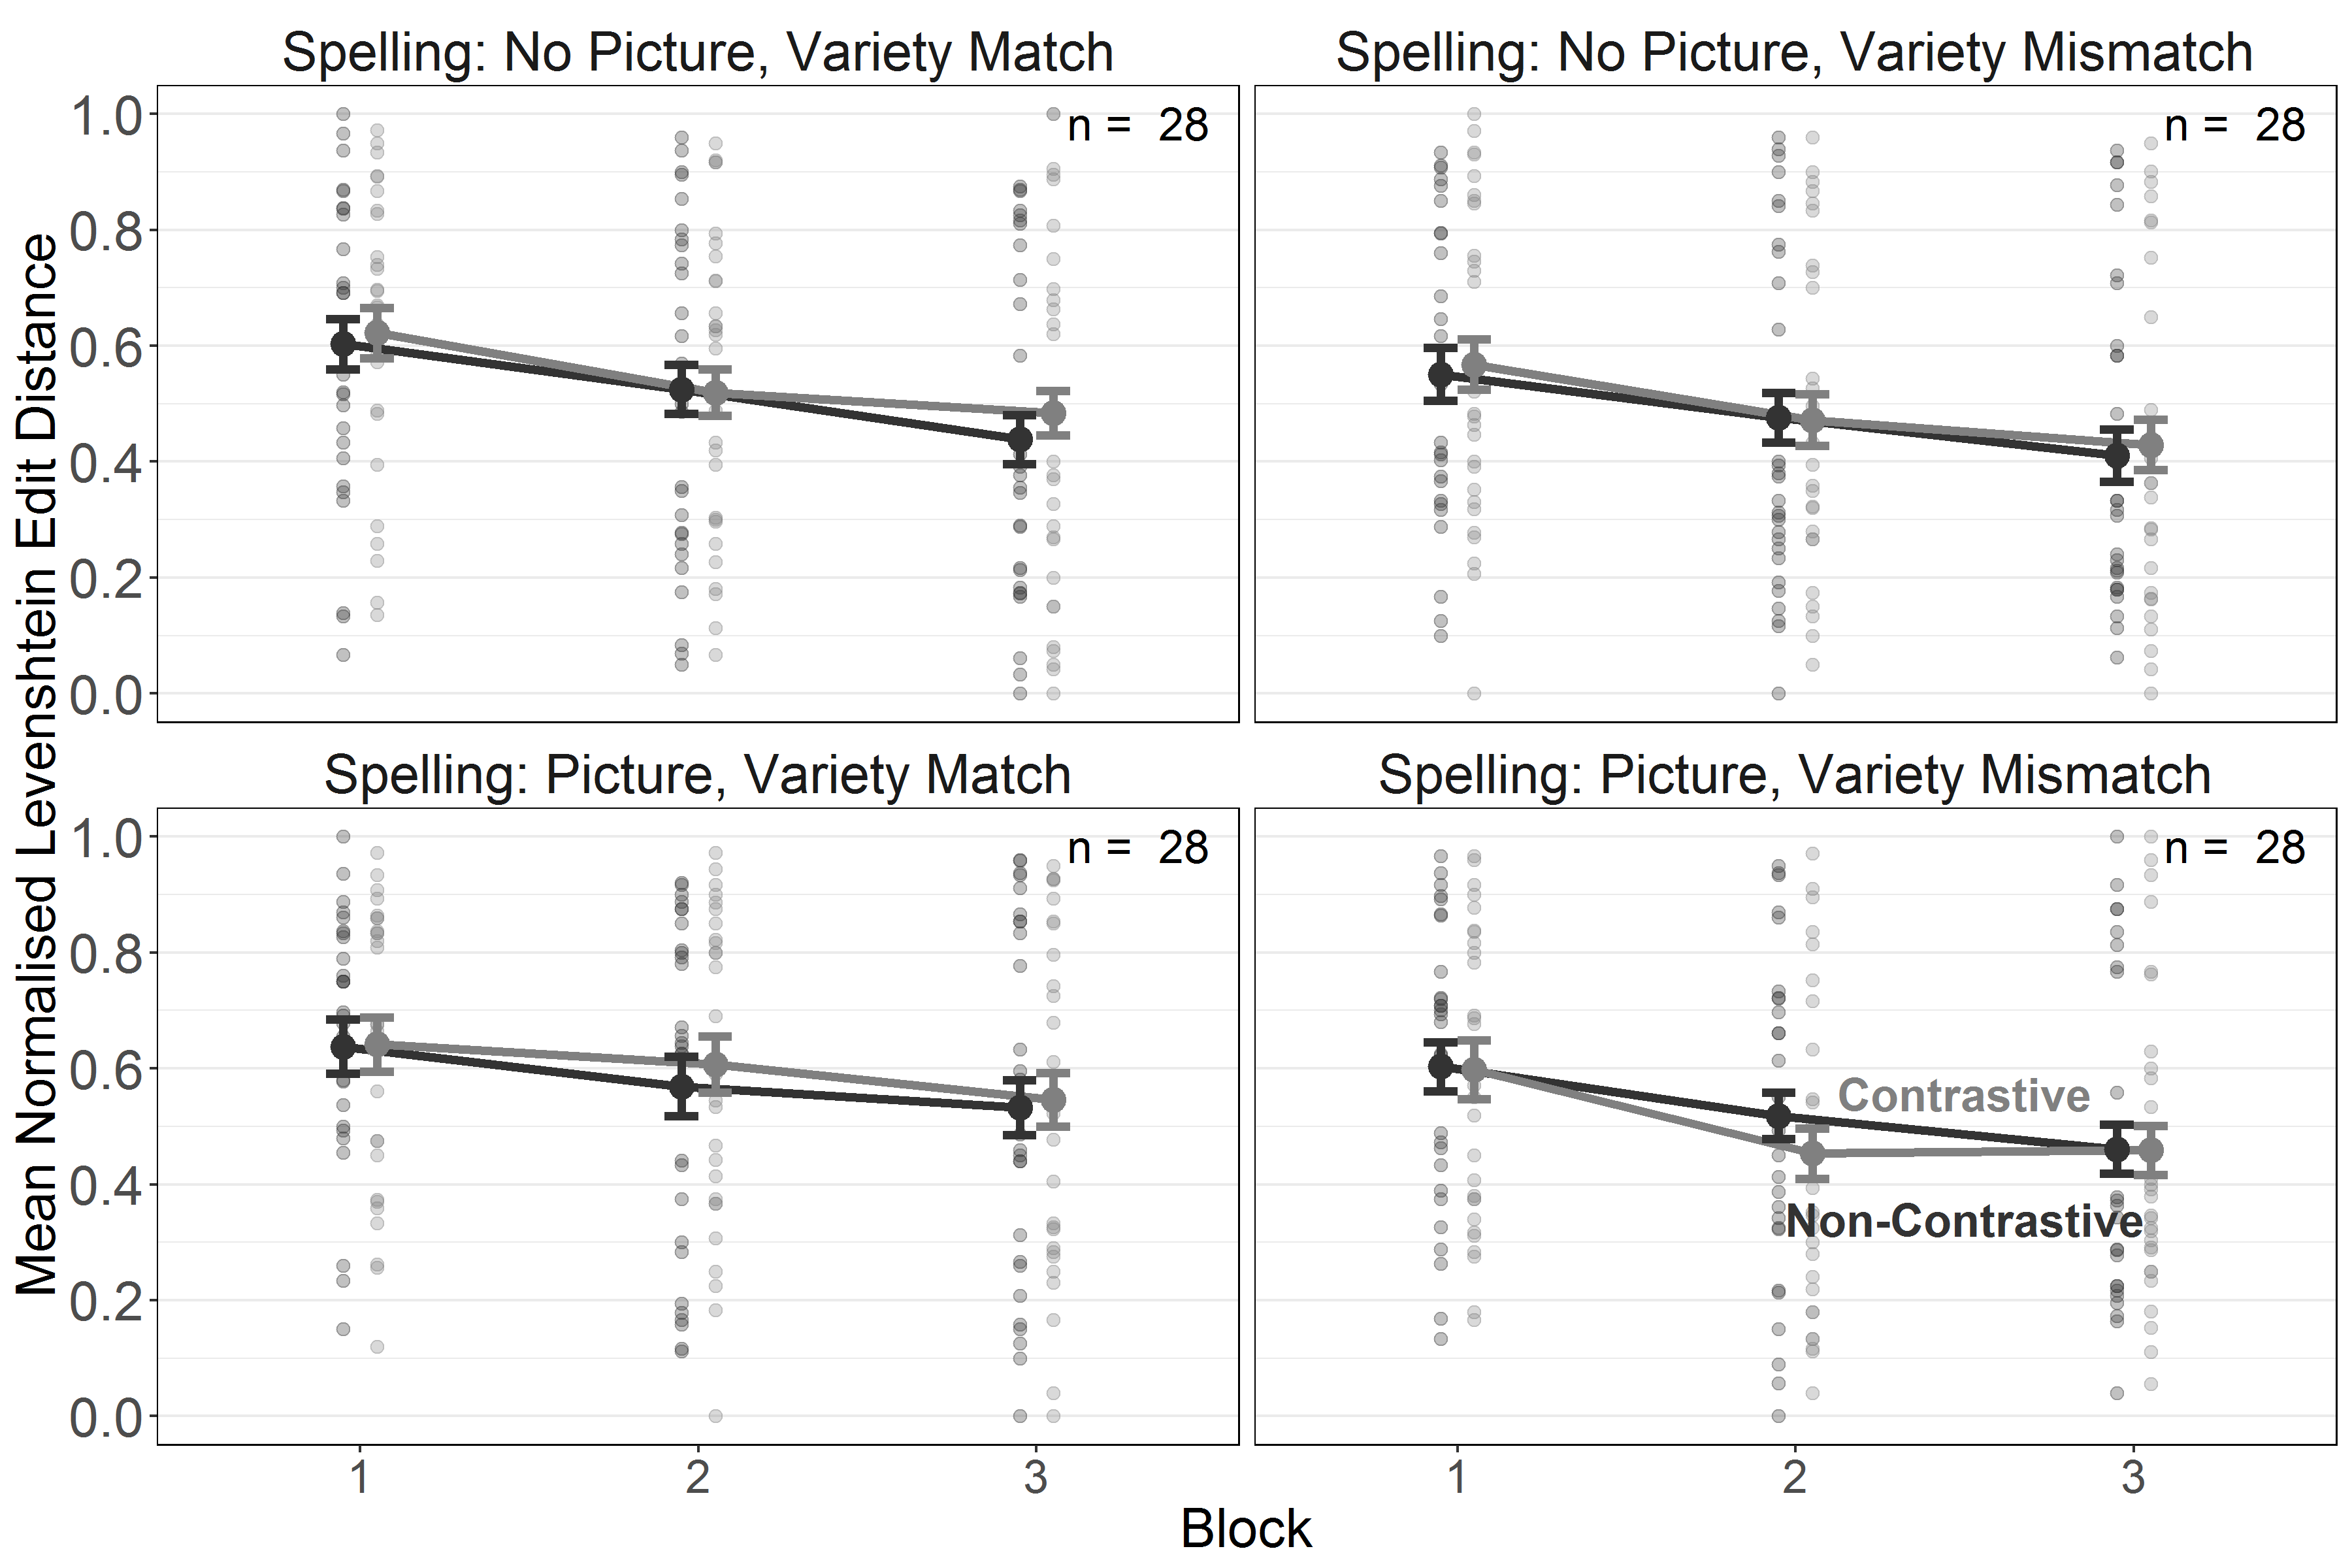
\includegraphics[width=1\linewidth]{C:/Users/g517364/Dropbox/GitHub/levenik/04_figures/output/experiment-2_training_plot_spelling} 

}

\caption{Experiment 2b. Length-normalised Levenshtein Edit Distance for spelling of contrastive and non-contrastive words during 3 training blocks in the variety match and variety mismatch conditions. Error bars indicate $\pm$ 1 $SE$ of the mean.}\label{fig:ex2-train-spelling-plots}
\end{figure}

\paragraph{Testing}\label{testing-2}

Parameter estimates, confidence intervals (for the frequentist analysis)
and credible intervals (for the Bayesian analysis) are presented in
Table~\ref{tab:ex2-test} and depicted in
Figures~\ref{fig:ex2-test-reading-plots} and
\ref{fig:ex2-test-spelling-plots}.

\begin{table}[!h]

\caption{\label{tab:ex2-test}Experiment 2b. Parameter estimates for the models fitted to nLEDs from the testing phase. Bayesian analyses report standardised parameter estimates (i.e. the intercept [grand mean] is centred at 0). Values of 0 with a sign indicate the direction of the estimate before rounding.}
\centering
\resizebox{\linewidth}{!}{
\fontsize{8}{10}\selectfont
\begin{tabular}{lrrlrlrrl}
\toprule
\multicolumn{1}{c}{ } & \multicolumn{5}{c}{Frequentist Estimates} & \multicolumn{3}{c}{Bayesian Estimates} \\
\cmidrule(l{3pt}r{3pt}){2-6} \cmidrule(l{3pt}r{3pt}){7-9}
Term & $Est.$ & $SE$ & 95\% Conf. I & $t$ & $p$ & $Est.$ & $SE$ & 95\% Cred. I\\
\midrule
Intercept & 0.69 & 0.04 & [0.61, 0.77] & 17.63 & < .001*** & 0.03 & 0.07 & [-0.11, 0.18]\\
\textbf{Task} & \textbf{-0.03} & \textbf{0.01} & \textbf{[-0.04, -0.02]} & \textbf{-4.10} & \textbf{< .001***} & \textbf{-0.06} & \textbf{0.01} & \textbf{[-0.09, -0.03]}\\
Picture Condition & 0.00 & 0.04 & [-0.07, 0.07] & 0.06 & 1.00 & 0.01 & 0.07 & [-0.12, 0.14]\\
Variety Condition & -0.05 & 0.04 & [-0.12, 0.02] & -1.31 & < .001*** & -0.08 & 0.07 & [-0.23, 0.06]\\
\textbf{TC $\times$ PC} & \textbf{0.02} & \textbf{0.01} & \textbf{[0.01, 0.04]} & \textbf{3.53} & \textbf{< .001***} & \textbf{0.05} & \textbf{0.01} & \textbf{[0.02, 0.07]}\\
TC $\times$ VC & -0.01 & 0.01 & [-0.02, 0.01] & -1.06 & < .001*** & -0.01 & 0.01 & [-0.04, 0.01]\\
PC $\times$ VC & 0.02 & 0.04 & [-0.06, 0.09] & 0.46 & 1.00 & 0.03 & 0.07 & [-0.10, 0.16]\\
TC $\times$ PC $\times$ VC & 0.00 & 0.01 & [-0.02, 0.01] & -0.47 & 1.00 & -0.01 & 0.01 & [-0.03, 0.02]\\
R, NP, VMis: WT & -0.01 & 0.02 & [-0.05, 0.03] & -0.34 & 1.00 & -0.01 & 0.04 & [-0.08, 0.07]\\
S, NP, VMis: WT & -0.02 & 0.02 & [-0.06, 0.02] & -0.98 & < .001*** & -0.03 & 0.04 & [-0.10, 0.04]\\
R, P, VMis: WT & -0.04 & 0.02 & [-0.08, -0.00] & -2.06 & < .001*** & -0.07 & 0.04 & [-0.15, 0.01]\\
S, P, VMis: WT & -0.01 & 0.02 & [-0.05, 0.03] & -0.39 & 1.00 & -0.01 & 0.04 & [-0.08, 0.06]\\
R, NP, VMa: WT & -0.02 & 0.02 & [-0.06, 0.02] & -0.99 & < .001*** & -0.03 & 0.04 & [-0.10, 0.04]\\
S, NP, VMa: WT & 0.00 & 0.02 & [-0.04, 0.04] & 0.02 & 1.00 & 0.01 & 0.04 & [-0.06, 0.07]\\
R, P, VMa: WT & -0.03 & 0.02 & [-0.07, 0.01] & -1.63 & < .001*** & -0.05 & 0.04 & [-0.13, 0.02]\\
S, P, VMa: WT & 0.00 & 0.02 & [-0.04, 0.04] & -0.08 & 1.00 & 0.00 & 0.03 & [-0.06, 0.07]\\
R, NP, VMis, WF & 0.01 & 0.02 & [-0.03, 0.04] & 0.44 & 1.00 & 0.01 & 0.04 & [-0.06, 0.08]\\
S, NP, VMis, WF & 0.01 & 0.02 & [-0.02, 0.04] & 0.61 & 1.00 & 0.02 & 0.03 & [-0.04, 0.08]\\
R, P, VMis, WF & 0.02 & 0.02 & [-0.01, 0.05] & 1.20 & < .001*** & 0.04 & 0.04 & [-0.03, 0.11]\\
S, P, VMis, WF & 0.01 & 0.02 & [-0.03, 0.04] & 0.32 & 1.00 & 0.01 & 0.03 & [-0.05, 0.07]\\
R, NP, VMa, WF & 0.02 & 0.02 & [-0.01, 0.05] & 1.08 & < .001*** & 0.03 & 0.03 & [-0.04, 0.10]\\
S, NP, VMa, WF & 0.01 & 0.02 & [-0.02, 0.04] & 0.53 & 1.00 & 0.01 & 0.03 & [-0.04, 0.07]\\
\textbf{R, P, VMa, WF} & \textbf{0.04} & \textbf{0.02} & \textbf{[0.01, 0.08]} & \textbf{2.54} & \textbf{< .001***} & \textbf{0.08} & \textbf{0.03} & \textbf{[0.01, 0.15]}\\
S, P, VMa, WF & 0.01 & 0.02 & [-0.02, 0.04] & 0.49 & 1.00 & 0.01 & 0.03 & [-0.04, 0.07]\\
\bottomrule
\multicolumn{9}{l}{Variety Condition (VC) = variety match vs. variety mismatch (VMa vs. VMi),}\\
\multicolumn{9}{l}{Picture Condition (PC) = picture vs. no picture (P vs. NP), Task Condition (TC) = reading vs. spelling (R vs. S),}\\
\multicolumn{9}{l}{Word Type (WT) = contrastive vs. non-contrastive, Word Familiarity (WF) = familiar vs. unfamiliar (novel)}\\
\end{tabular}}
\end{table}

The results confirmed the interaction between Task and Picture Condition
found already in the training data which suggests that reading
performance was better than writing performance in the picture condition
only (Picture, Reading - Writing: \(\Delta{M}\) = -0.11{[}-0.16,
-0.05{]}, \emph{t} = -5.40, \emph{p} = \textless{} .001). However,
unlike Experiment 2b, there was no contrastive deficit and the effect of
word familiarity appeared only in one condition, i.e.~during reading in
the Variety Match condition with pictures.

\begin{figure}[htb]

{\centering 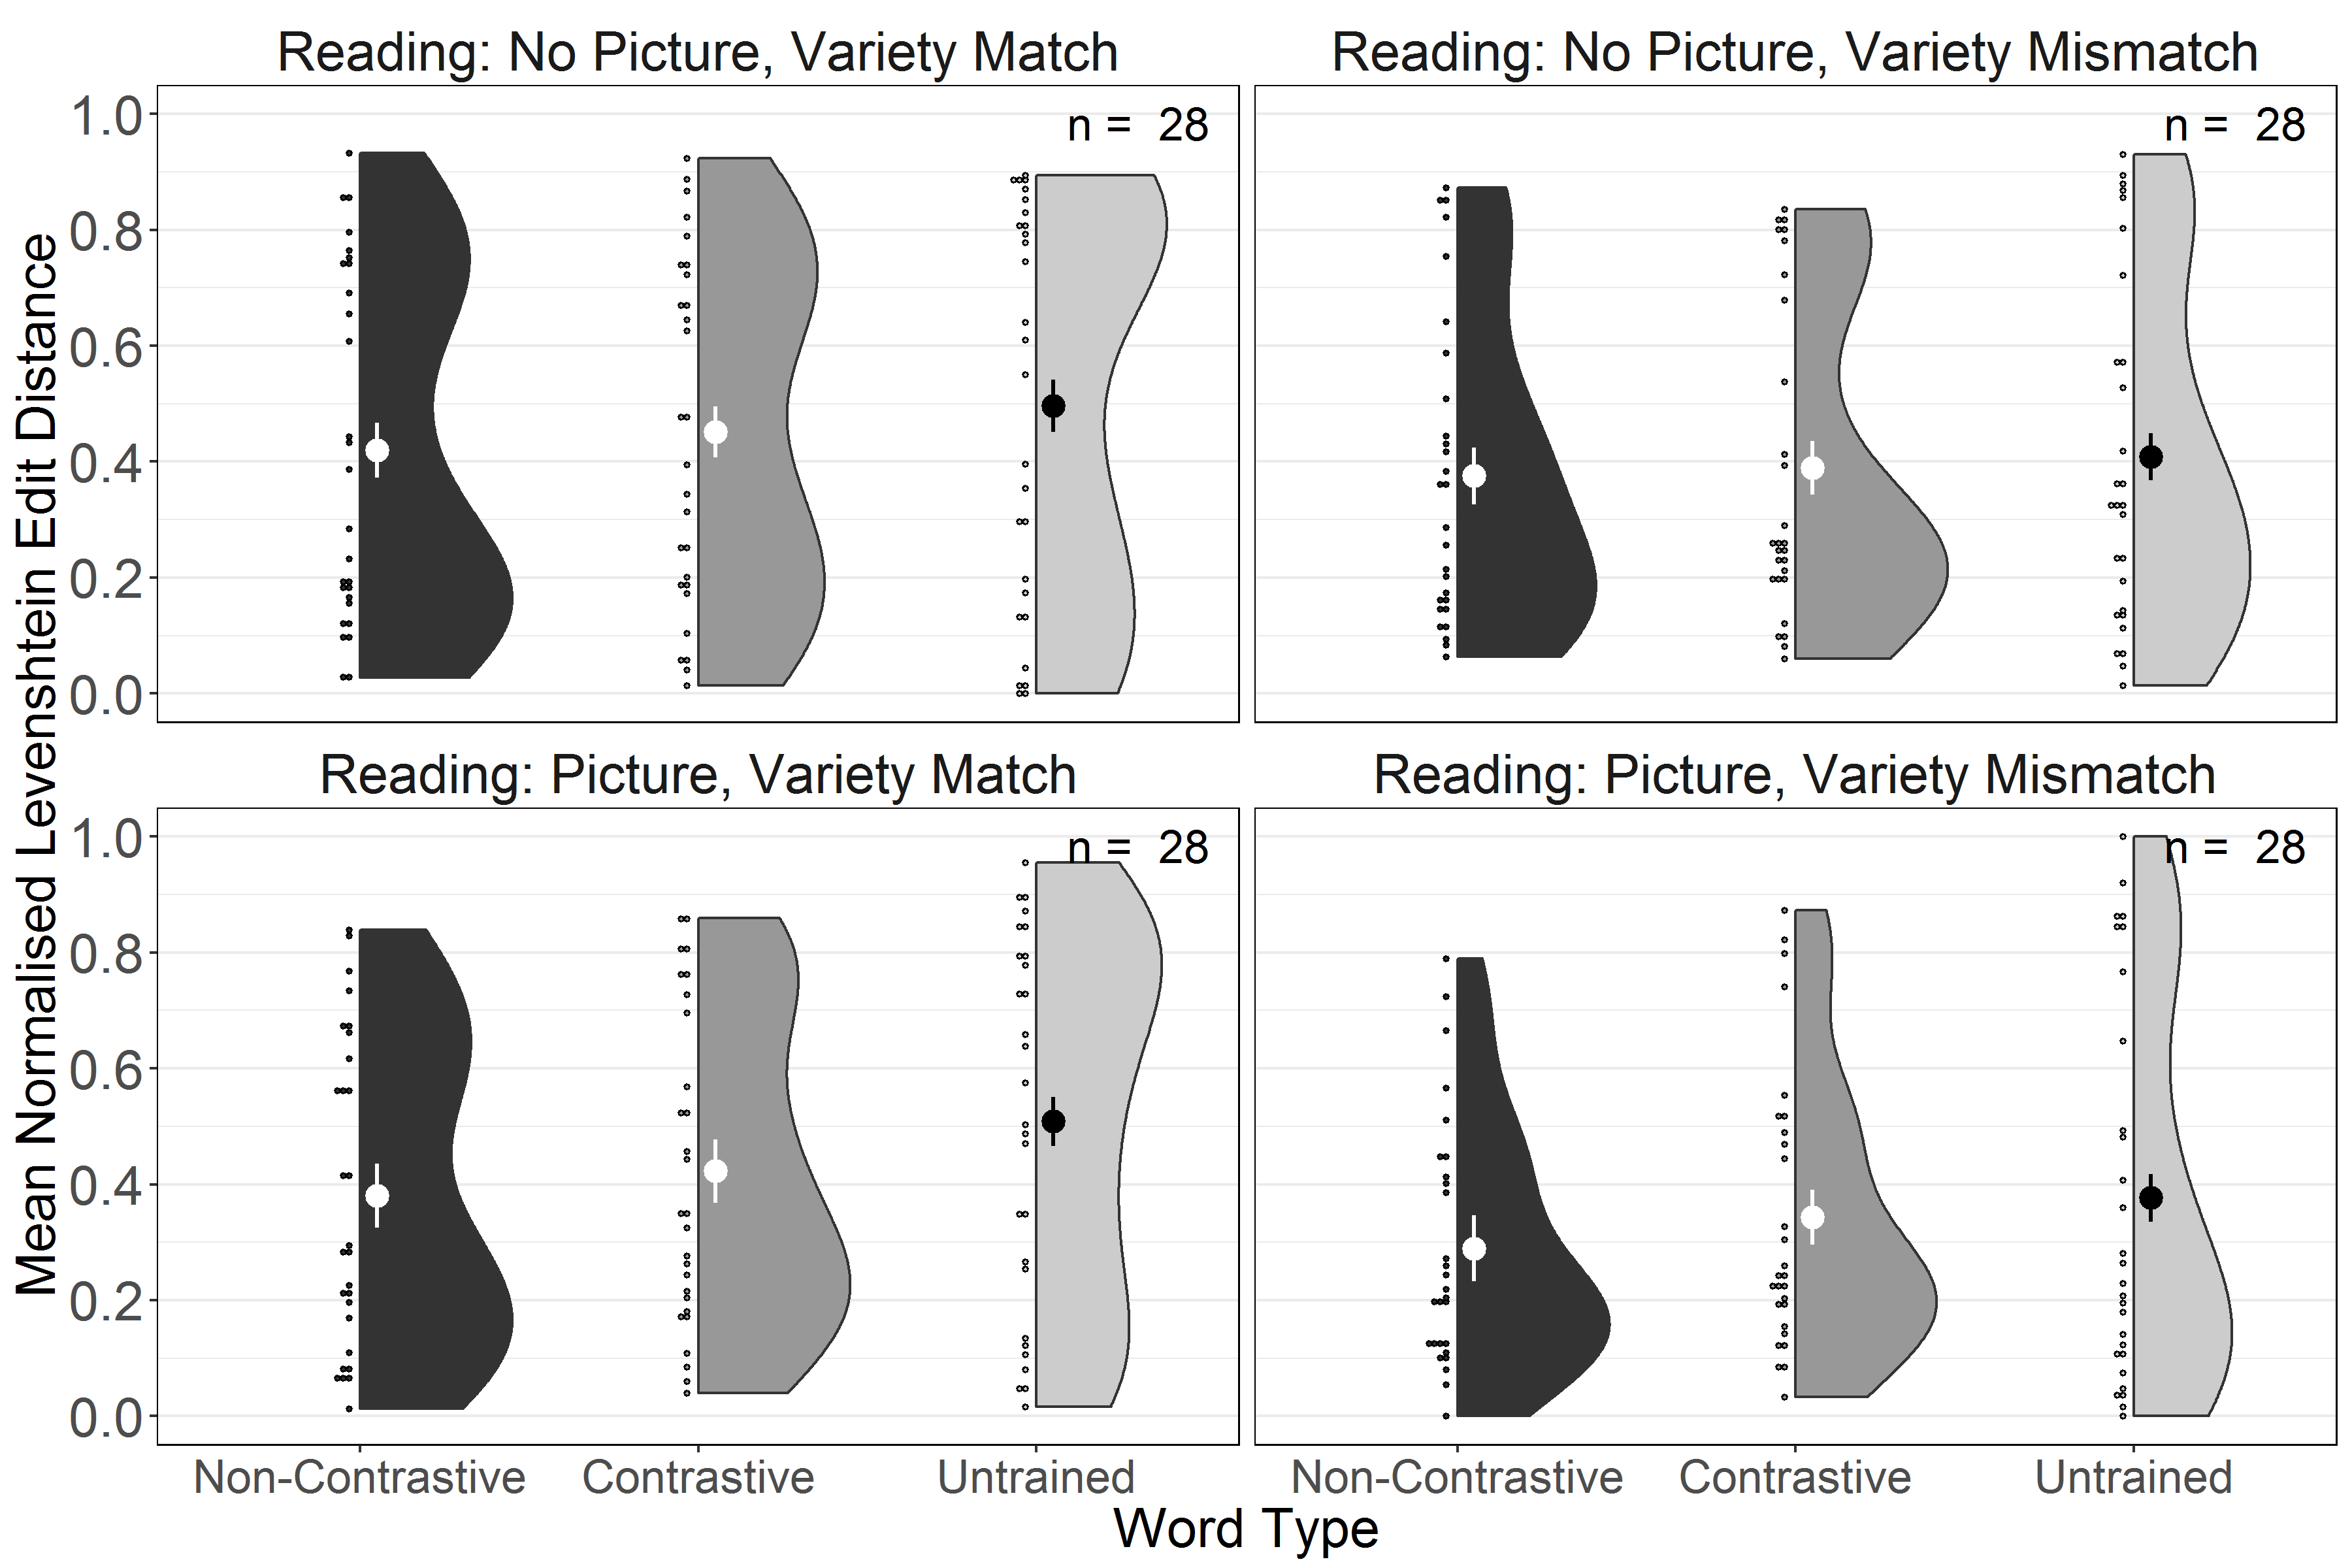
\includegraphics[width=1\linewidth]{C:/Users/g517364/Dropbox/GitHub/levenik/04_figures/output/experiment-2_testing_plot_reading} 

}

\caption{Experiment 2b. Length-normalised Levenshtein Edit Distance for testing reading performance for trained non-contrastive, trained contrastive and untrained words in the variety match and variety mismatch conditions. Large dots and whiskers indicate means and $\pm$ 1 $SE$ of the mean.}\label{fig:ex2-test-reading-plots}
\end{figure}

\begin{figure}[htb]

{\centering 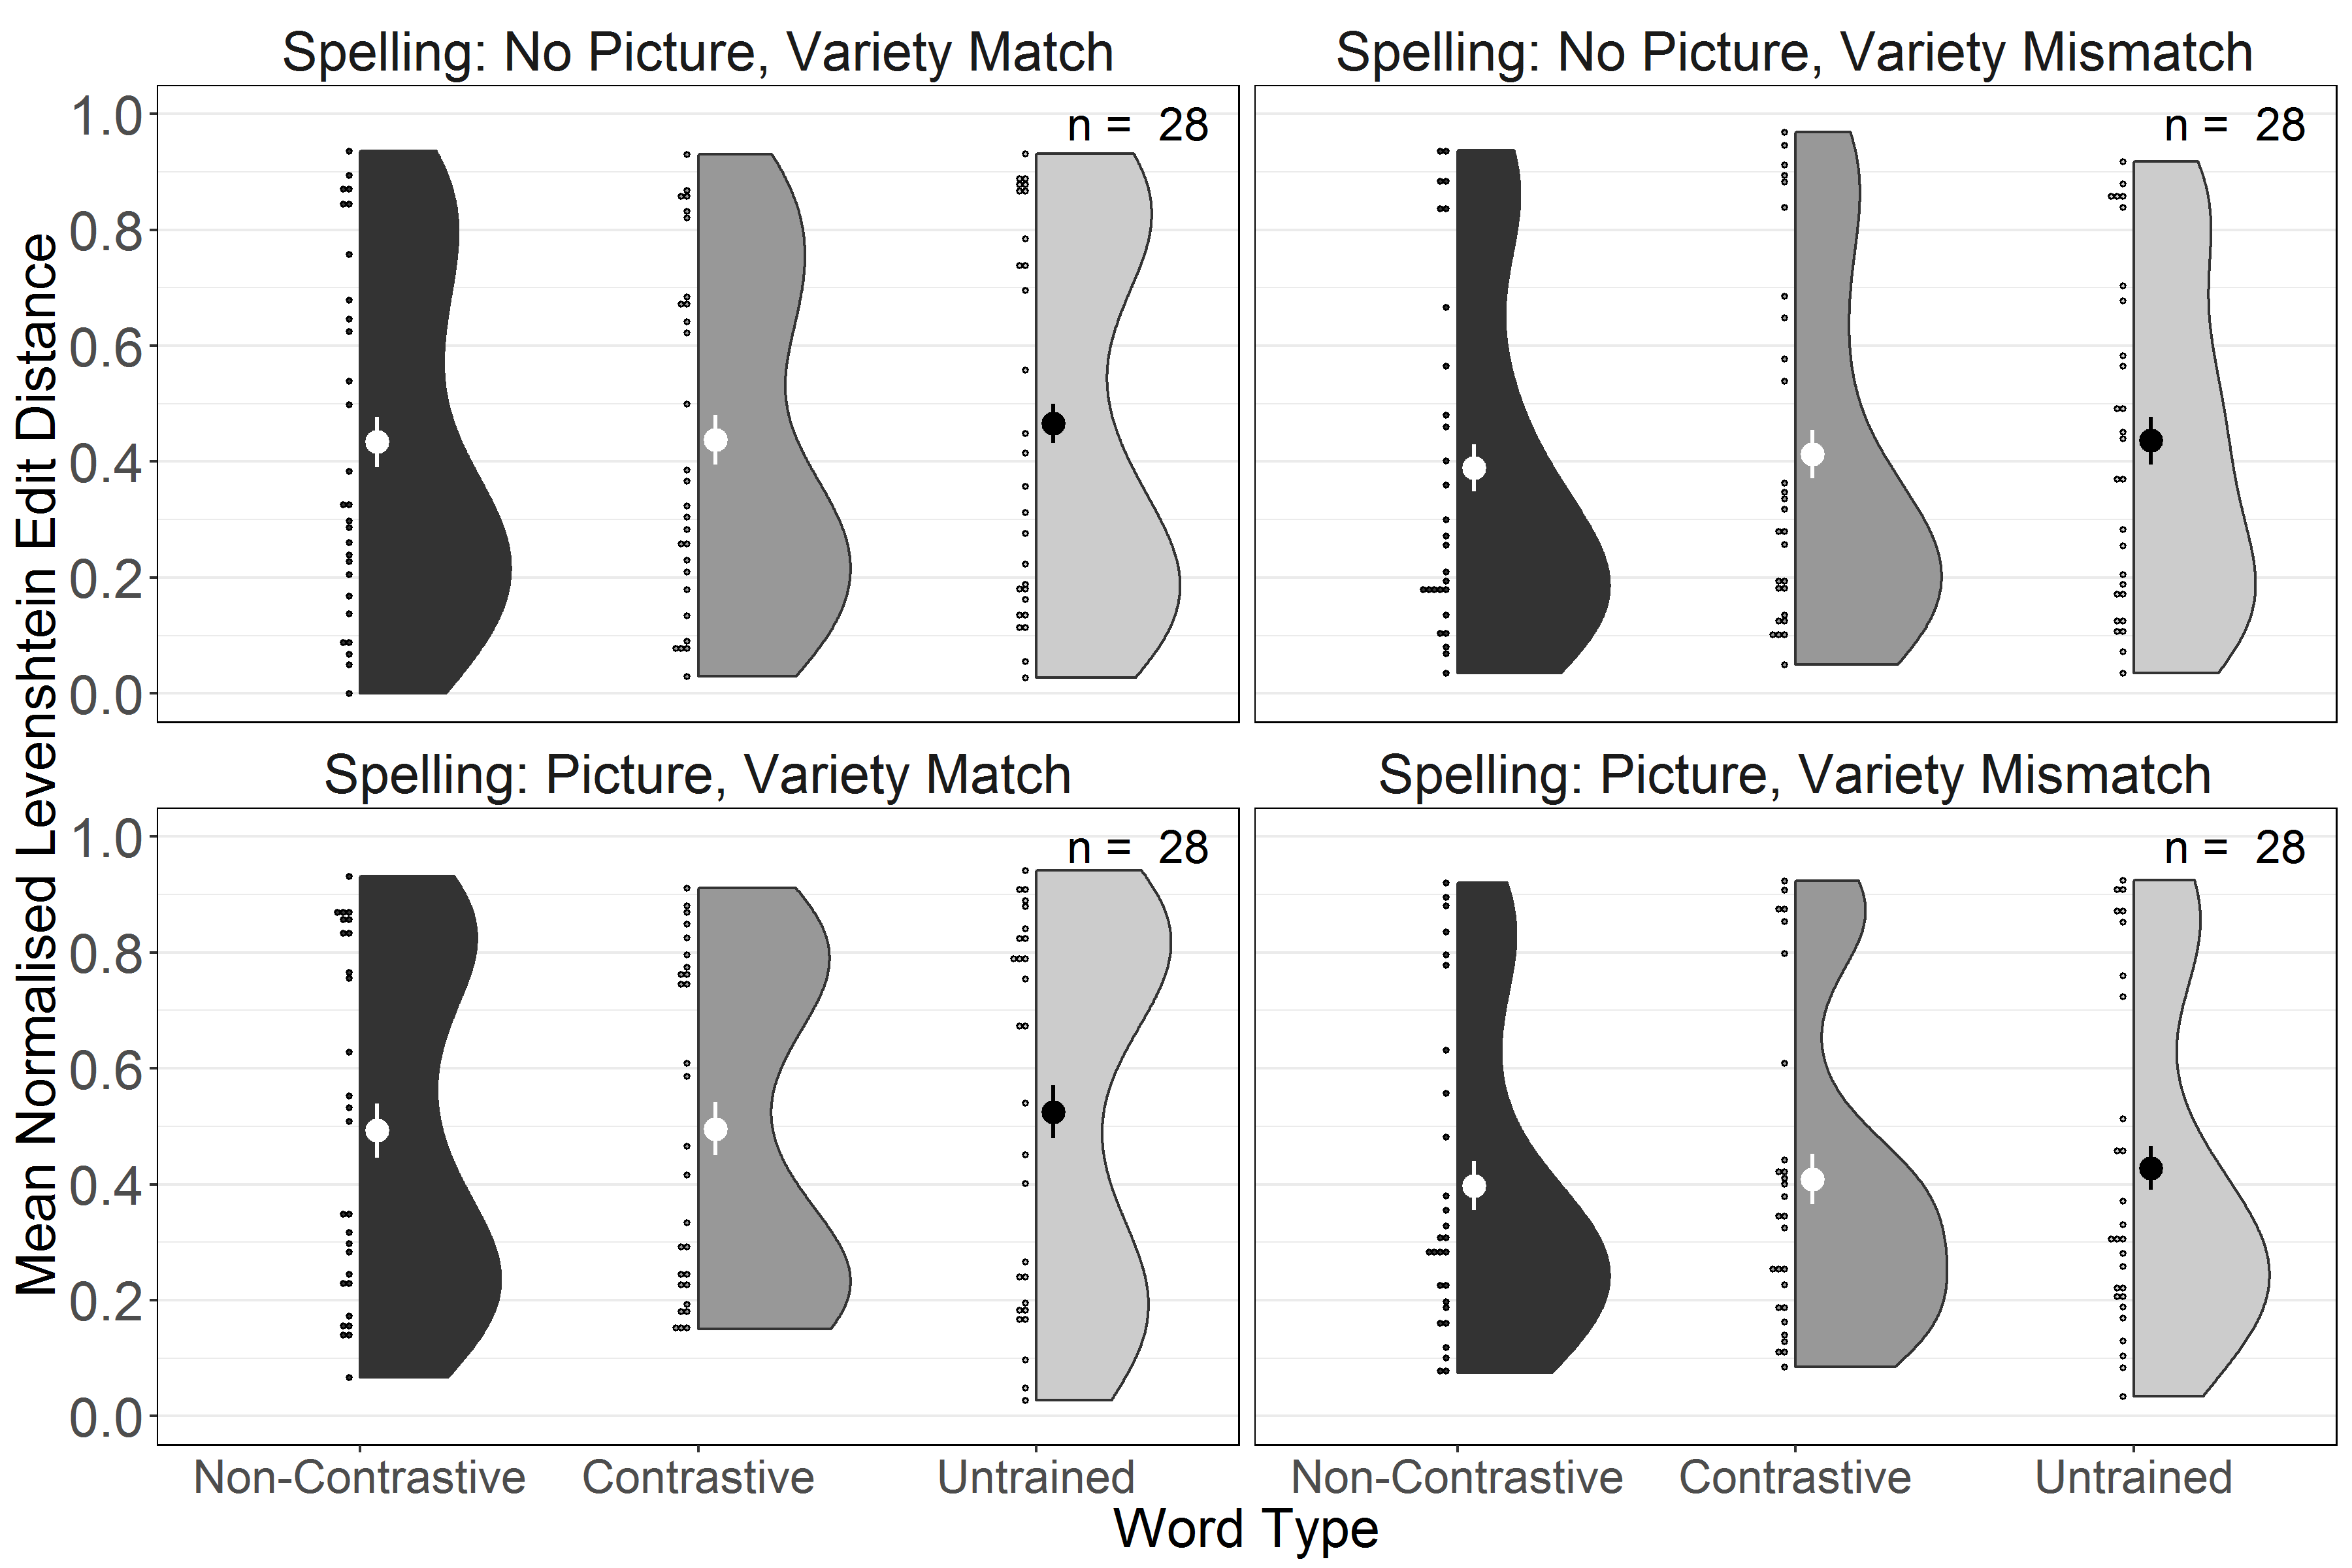
\includegraphics[width=1\linewidth]{C:/Users/g517364/Dropbox/GitHub/levenik/04_figures/output/experiment-2_testing_plot_spelling} 

}

\caption{Experiment 2b. Length-normalised Levenshtein Edit Distance for testing spelling performance for trained non-contrastive, trained contrastive and untrained words in the variety match and variety mismatch conditions. Large dots and whiskers indicate means and $\pm$ 1 $SE$ of the mean.}\label{fig:ex2-test-spelling-plots}
\end{figure}

The planned comparison of performance on untrained words only between
all Variety Match and Variety Mismatch conditions used the same model
structure as for Experiment 2a. There was no effect of Variety
(frequentist estimate: \(\hat{\beta}\) = -0.06{[}-0.14, 0.02{]},
\emph{t} = -1.38, \emph{p} = \textless{} .001***; Bayesian Estimate:
\(\hat{\beta}\) = -0.09{[}-0.25, 0.07{]}), again suggesting that there
was no evidence for a deterimental effect of exposure to a variety
mismatch on reading and spelling of untrained words.

\subsection{Discussion}\label{discussion-2}

When attempting to learn to read and to spell an opaque artificial
orthography participants showed improvement over the course of training.
However, unlike in Experiment 1, where the contrastive deficit was found
in some of the Variety Mismatch conditions, there was no effect of Word
Type in this experiment. This suggests that learning conditional
spelling rules has rendered literacy acquisition in an opaque
orthography too difficult for phonological representations that could
have been placed into competition with each other to emerge. This
confirms observations from cross-linguistic studies of literacy
acquisition in naturalistic settings which show that literacy
acquisition at the early stages is more difficult for opaque compared to
transparent orthographies (Seymour, Aro, \& Erskine, 2003). It would
seem, then, that under these conditions participants did not acquire any
decoding skills and -- consequently -- no effect of variety mismatch on
reading and spelling of untrained words was observed.

Although this was not the main aim of this study, the first three
experiments combined give us the opportunity to explore which conditions
are most conducive to literacy acquisition.
Figure~\ref{fig:ex1-to-2-test-plots} shows a direct comparison of
reading performance for all trained and untrained items during testing
in the three experiments.

\begin{figure}[htb]

{\centering 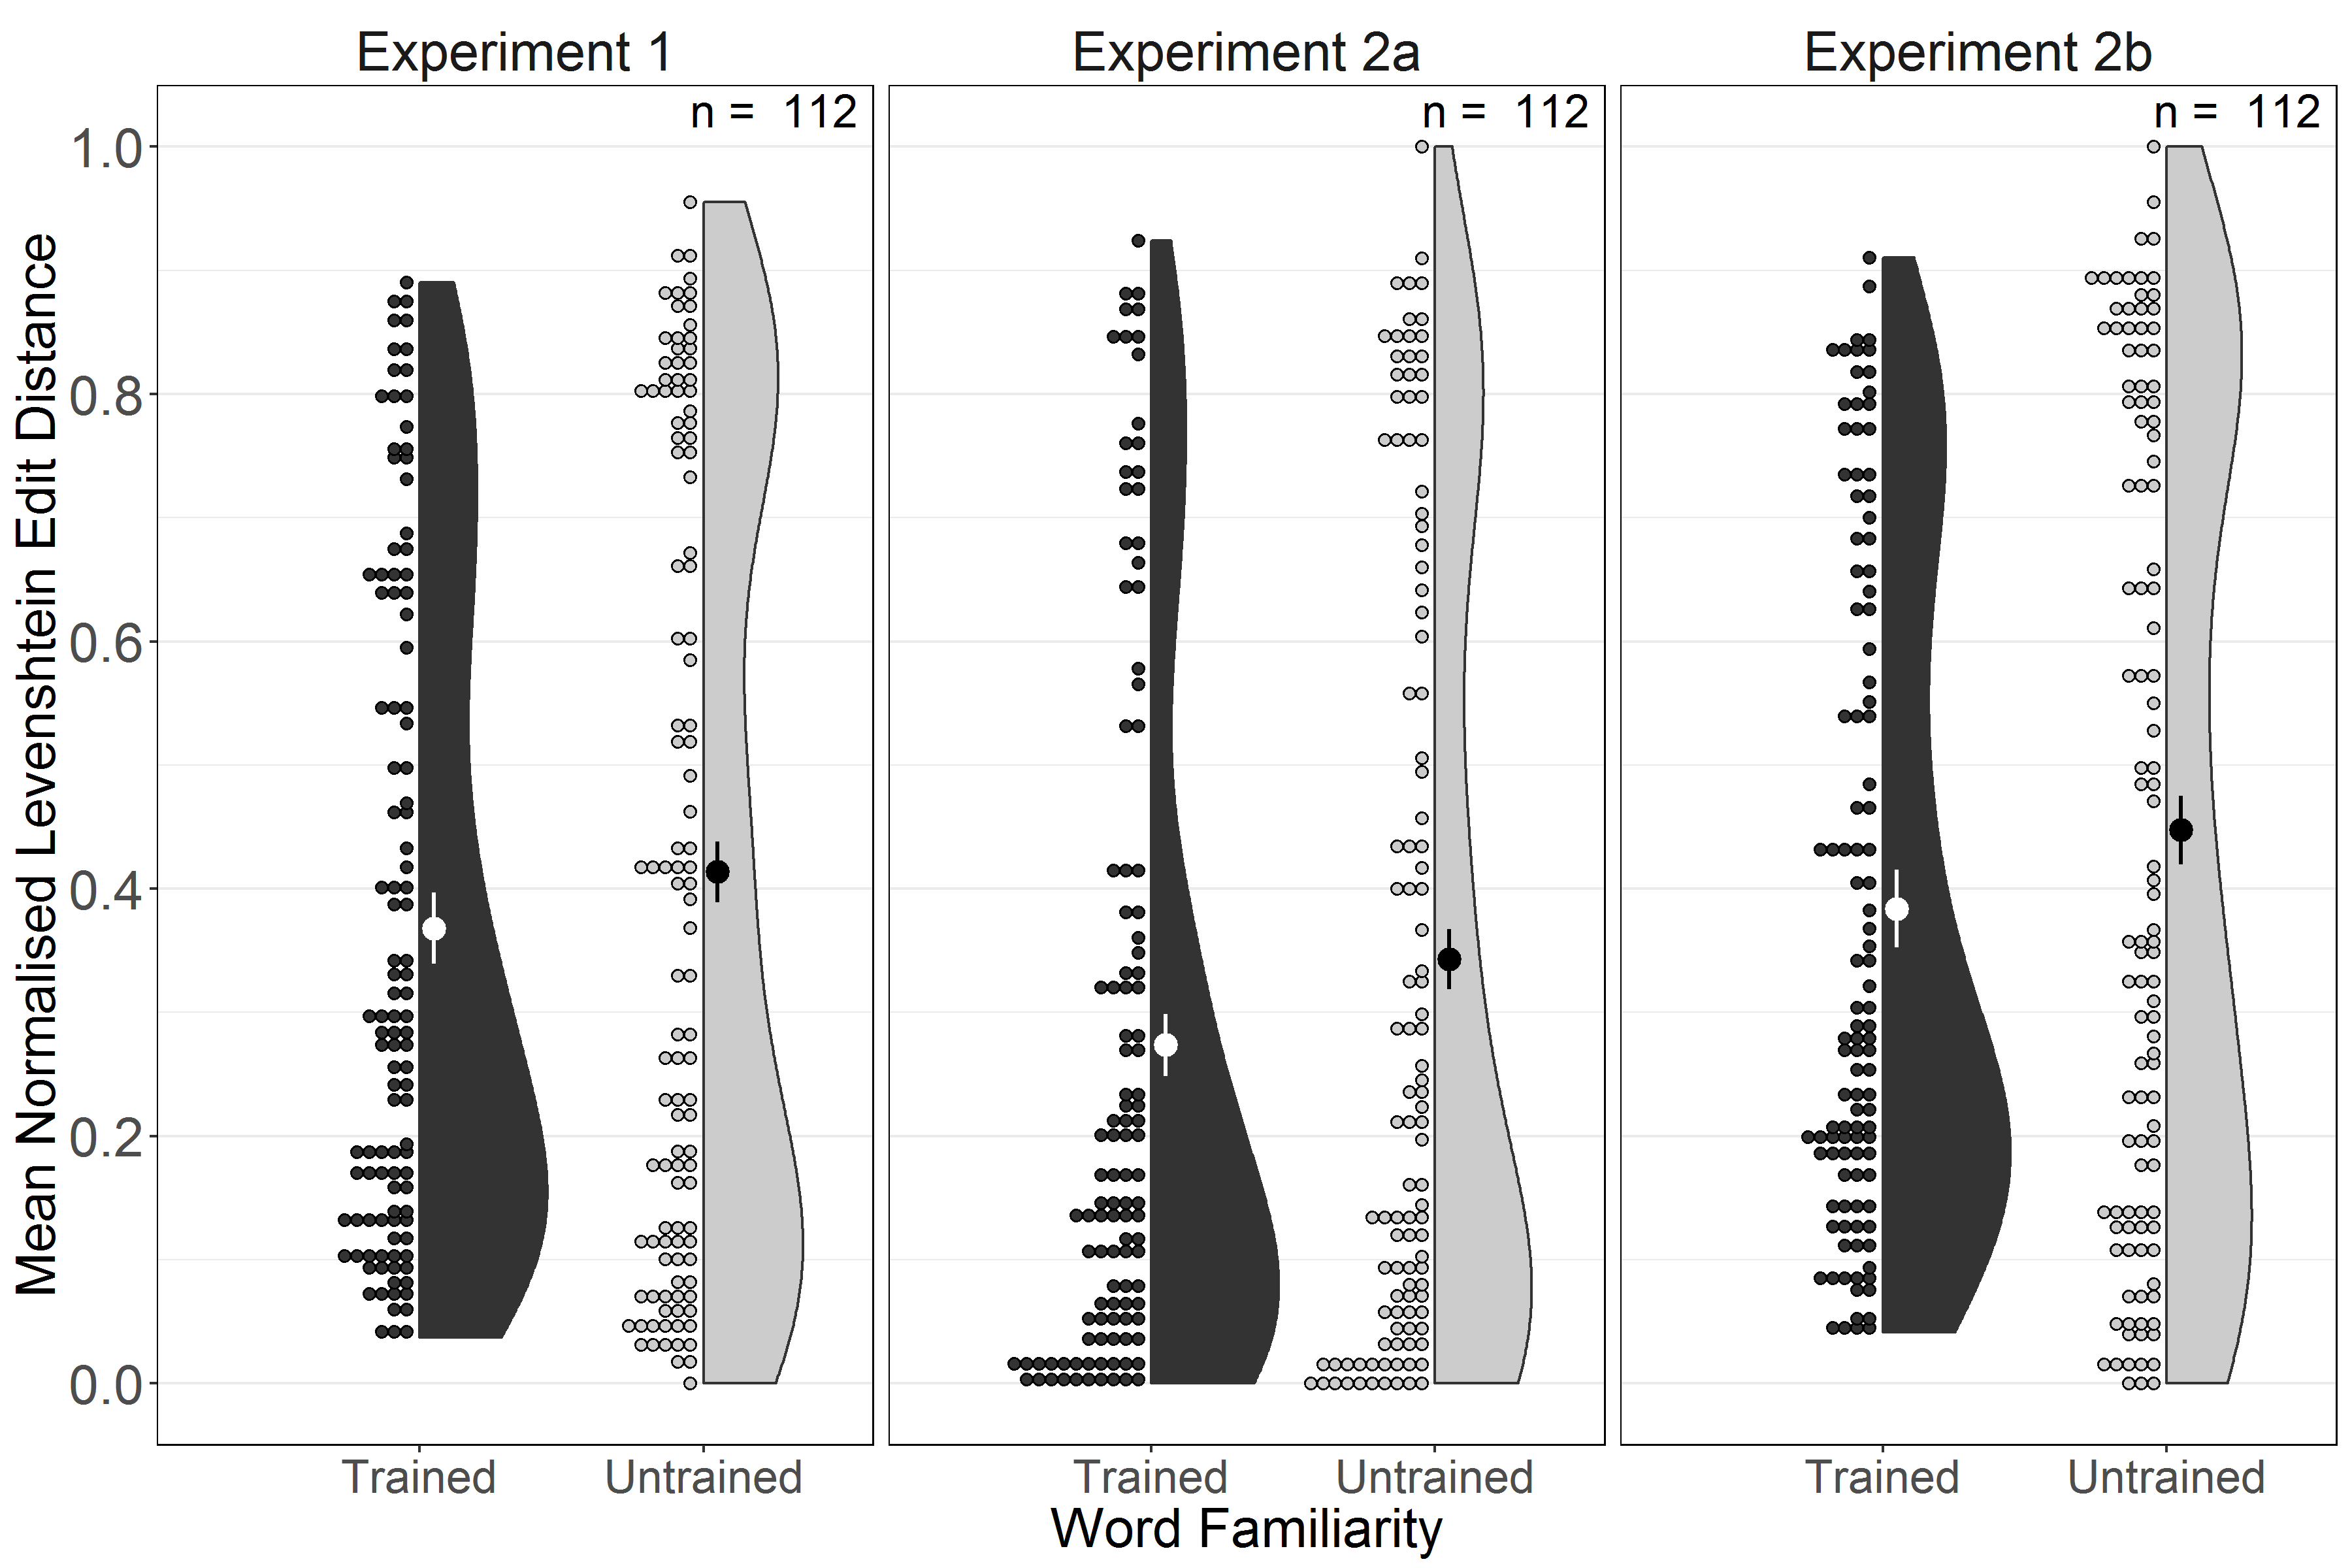
\includegraphics[width=1\linewidth]{C:/Users/g517364/Dropbox/GitHub/levenik/04_figures/output/experiments-1-to-2_word-novelty} 

}

\caption{\textit{Experiments 1 \& 2. Length-normalised Levenshtein Edit Distance for testing performance across both tasks for trained and untrained words. Large dots and whiskers indicate means and $\pm$ 1 $SE$ of the mean.}}\label{fig:ex1-to-2-test-plots}
\end{figure}

We first fitted a linear mixed effect model with sum-coded fixed effects
of Word Familiarity and treatment-coded fixed effects Experiment (1, 2a,
2b), and with a maximal random effects structure of random intercepts
and slopes of Experiment by item and random intercepts and slopes of
Word Familiarity by subjects. Pairwise contrasts were then calculated
for each experiment split by Word Familiarity based on the estimated
marginal means from the model using the \emph{emmeans} R-package(Lenth,
2019). Here, \emph{p}-values are adjusted using Holm's sequential
Bonferroni correction.

\begin{table}[!h]

\caption{\label{tab:ex1-to-2-test}Experiments 1 \& 2. Parameter estimates for pairwise contrasts between Experiments 1, 2a, and 2b split by Word Familiarity in the testing phase.}
\centering
\resizebox{\linewidth}{!}{
\fontsize{8}{10}\selectfont
\begin{tabular}{lrrlrl}
\toprule
Contrast & $\Delta M$ & $SE$ & 95\% Conf. I & $t$ & $p$\\
\midrule
\addlinespace[0.3em]
\multicolumn{6}{l}{Trained Words}\\
\hspace{1em}\hspace{1em}\textbf{Experiment 0 - Experiment 1} & \textbf{0.09} & \textbf{0.02} & \textbf{[0.05, 0.13]} & \textbf{5.82} & \textbf{< .001}\\
\hspace{1em}\hspace{1em}Experiment 0 - Experiment 2 & -0.06 & 0.05 & [-0.18, 0.05] & -1.34 & .181\\
\hspace{1em}\hspace{1em}\textbf{Experiment 1 - Experiment 2} & \textbf{-0.16} & \textbf{0.05} & \textbf{[-0.27, -0.04]} & \textbf{-3.22} & \textbf{.003}\\
\addlinespace[0.3em]
\multicolumn{6}{l}{Untrained Words}\\
\hspace{1em}\hspace{1em}Experiment 0 - Experiment 1 & 0.06 & 0.03 & [-0.00, 0.12] & 2.42 & .061\\
\hspace{1em}\hspace{1em}Experiment 0 - Experiment 2 & -0.07 & 0.05 & [-0.20, 0.06] & -1.30 & .193\\
\hspace{1em}\hspace{1em}Experiment 1 - Experiment 2 & -0.13 & 0.06 & [-0.27, 0.00] & -2.32 & .061\\
\bottomrule
\end{tabular}}
\end{table}

These contrasts show that for trained words, performance was better in
Experiment 1 than in Experiment 0. Additionally, performance was also
better in Experiment 1 than in Experiment 2. All other contrasts were
non-significant. This suggests that while introduction of spelling had
no effect on overall learning outcomes, learning a transparent
orthography lead to measurable benefits compared to learning an opaque
orthography, regardless of spelling, but only for trained and not for
untrained words. Recall that it was the transparent orthography for
which the contrastive deficit emerged most consistently. This suggests
that competition between variants will appear only once learning has
progressed to a stage at which access to phonological representations,
either via decoding of the the graphemic form or via semantic
representations, have been established. The considerable variability in
performance, illustrated in all figures, compellingly shows that
participants differ tremendously in terms of their success in the early
stages of this process. Thus, to create conditions that would allow for
more reliable emergence of phonological representations, Experiment 3
repeated Experiment 2b with a longer training phase and a larger sample
of learners.

\section{Experiment 3}\label{experiment-3}

\subsection{Method}\label{method-3}

\subsubsection{Participants}\label{participants-3}

One hundred and sixty participants (aged aged 18--61, \emph{M} = 32.48,
\emph{SD} = 9.67) were recruited online through Prolific Academic and
took part in the study for \pounds 9. All participants reported
proficiency in English (1-7 Likert scale: \emph{M} = 4.86, \emph{SD} =
0.58). Another 6 participants were tested and excluded based on the
exclusion criteria described for Experiment 1.

\subsubsection{Materials}\label{materials-3}

We used the same materials as in Experiments 1, 2a, and 2b, and the same
opaque orthography as in Experiments 1 and 2b.

\subsubsection{Procedure}\label{procedure-3}

The procedure deviated from Experiment 2a and 2b in that the training
phase was doubled in length by adding another three ten-word
double-blocks (i.e.~blocks comprising the same ten words in the reading
and the spelling task with order of tasks counterbalanced across
participants) resulting in a total of six double-blocks. All words were
first partitioned for presentation in the first three double-blocks and
then re-partitioned for presentation in the final three double-blocks,
ensuring that each double-block contained five contrastive and five
non-contrastive words.

As Experiment 2a had suggested that contrastive deficits are likely to
persist longer in the Picture condition, presumably because participants
associated the two variants of each contrastive words with the same
concept, all words were presented along with an associated picture of a
concrete object during exposure and reading training. The mean
completion time was 98.14 minutes (\emph{SD} = 91.20).

\subsection{Results}\label{results-3}

\subsubsection{Coding}\label{coding-3}

We used the same coding scheme for reading responses as in the previous
experiments. The ICC between coders was F(32267.00, 32202.82) = 85.81,
\(p\) \textless{} .001, ICC = 0.98 {[}95\% CI = 0.98; 0.98{]}. The 95\%
confidence interval around the parameter estimate indicates that the ICC
falls above the bound of .90, which suggests excellent reliability
across raters (see Koo \& Li, 2016).

\subsubsection{Model Fitting}\label{model-fitting-3}

We used the a similar model structure to Experiments 2a and b, with the
exclusion of the Picture condition factor. As in Experiments 1, 2a, and
2b, the fixed effects for training and testing were modelled by
obtaining all main effects and interactions between all factors
excluding Word Type and nesting Word Type within each combination of
factor levels of Task and Variety Condition. Because this experiment,
like Experiment 1, contained six blocks per task, we included the
quadratic term for Block in the analyses of the training data to improve
model fit.

The maximal converging random effects structure took the form of
zero-correlation random intercepts and slopes of Task, Variety
Condition, and their interaction by items, and random intercepts and
slopes for the linear and quadratic time terms, Task, Word Type, and
their interaction by subjects, including all correlations between these
terms. For the testing data, the random effects structure took the form
of random intercepts and slopes of Task, Variety Condition, and their
interaction by items, and random intercepts and slopes for Task, Word
Type, and their interaction by subjects, including all correlations
between these terms for both by-subjects and by-items random effects.

As with Experiments 1, 2a, and 2b, we also modelled the data using
Bayesian mixed effects models with a full \enquote{maximal} random
effects structure (i.e.~without suppressing correlations between the
by-items random effects in the training phase). These models used the
same priors as in Experiments 2a and 2b, with the inclusion of a
regularising, very weakly informative prior, \(Normal(0, 10)\), on the
orthogonal quadratic time term, excluding priors for Picture Condition
which was no longer in the model. We used these models to evaluate
evidence in support of the null hypothesis for each parameter in the
same way as in Experiments 1, 2a, and 2b.

\paragraph{Training}\label{training-3}

Parameter estimates, confidence intervals (for the frequentist analysis)
and credible intervals (for the Bayesian analysis) are presented in
Table~\ref{tab:ex3-train} and depicted in
Figures~\ref{fig:ex3-train-reading-plots} and
\ref{fig:ex3-train-spelling-plots}.

\begin{table}[!h]

\caption{\label{tab:ex3-train}Experiment 3. Parameter estimates for the models fitted to nLEDs from the training phase. Bayesian analyses report standardised parameter estimates (i.e. the intercept [grand mean] is centred at 0). Values of 0 with a sign indicate the direction of the estimate before rounding.}
\centering
\resizebox{\linewidth}{!}{
\fontsize{8}{10}\selectfont
\begin{tabular}{lrrlrlrrl}
\toprule
\multicolumn{1}{c}{ } & \multicolumn{5}{c}{Frequentist Estimates} & \multicolumn{3}{c}{Bayesian Estimates} \\
\cmidrule(l{3pt}r{3pt}){2-6} \cmidrule(l{3pt}r{3pt}){7-9}
Term & $Est.$ & $SE$ & 95\% Conf. I & $t$ & $p$ & $Est.$ & $SE$ & 95\% Cred. I\\
\midrule
Intercept & 0.73 & 0.03 & [0.67, 0.78] & 25.01 & < .001*** & 0.05 & 0.06 & [-0.06, 0.15]\\
\textbf{Block} & \textbf{-17.99} & \textbf{0.86} & \textbf{[-19.68, -16.30]} & \textbf{-20.84} & \textbf{< .001***} & \textbf{-0.63} & \textbf{0.03} & \textbf{[-0.68, -0.56]}\\
\textbf{Block$^2$} & \textbf{5.23} & \textbf{0.59} & \textbf{[4.07, 6.39]} & \textbf{8.84} & \textbf{< .001***} & \textbf{0.18} & \textbf{0.02} & \textbf{[0.14, 0.22]}\\
\textbf{Task} & \textbf{-0.05} & \textbf{0.01} & \textbf{[-0.07, -0.03]} & \textbf{-5.50} & \textbf{< .001***} & \textbf{-0.10} & \textbf{0.02} & \textbf{[-0.13, -0.06]}\\
Variety Condition & -0.03 & 0.03 & [-0.08, 0.02] & -1.05 & < .001*** & -0.05 & 0.05 & [-0.15, 0.04]\\
\textbf{B $\times$ TC} & \textbf{-1.96} & \textbf{0.49} & \textbf{[-2.91, -1.00]} & \textbf{-4.01} & \textbf{< .001***} & \textbf{-0.07} & \textbf{0.02} & \textbf{[-0.10, -0.03]}\\
B$^2$ $\times$ TC & 0.43 & 0.42 & [-0.38, 1.25] & 1.04 & < .001*** & 0.01 & 0.01 & [-0.01, 0.04]\\
B $\times$ VC & -1.70 & 0.86 & [-3.39, -0.01] & -1.97 & < .001*** & -0.06 & 0.03 & [-0.12, 0.00]\\
\textbf{B$^2$ $\times$ VC} & \textbf{1.71} & \textbf{0.59} & \textbf{[0.55, 2.87]} & \textbf{2.88} & \textbf{< .001***} & \textbf{0.06} & \textbf{0.02} & \textbf{[0.02, 0.10]}\\
TC $\times$ VC & 0.01 & 0.01 & [-0.00, 0.03] & 1.37 & < .001*** & 0.02 & 0.01 & [-0.01, 0.05]\\
\textbf{B $\times$ TC $\times$ VC} & \textbf{1.00} & \textbf{0.49} & \textbf{[0.04, 1.95]} & \textbf{2.04} & \textbf{< .001***} & \textbf{0.03} & \textbf{0.02} & \textbf{[0.00, 0.07]}\\
B$^2$ $\times$ TC $\times$ VC & -0.45 & 0.42 & [-1.26, 0.37] & -1.08 & < .001*** & -0.02 & 0.01 & [-0.04, 0.01]\\
\textbf{R, VMis: WT} & \textbf{-0.04} & \textbf{0.02} & \textbf{[-0.07, -0.01]} & \textbf{-2.61} & \textbf{< .001***} & \textbf{-0.07} & \textbf{0.03} & \textbf{[-0.13, -0.01]}\\
S, VMis: WT & 0.00 & 0.02 & [-0.03, 0.03] & -0.06 & 1.00 & 0.00 & 0.03 & [-0.06, 0.07]\\
R, VMa: WT & -0.02 & 0.02 & [-0.05, 0.01] & -1.23 & < .001*** & -0.03 & 0.03 & [-0.09, 0.03]\\
S, VMa: WT & 0.00 & 0.02 & [-0.03, 0.03] & -0.15 & 1.00 & 0.00 & 0.03 & [-0.06, 0.06]\\
B, R, VMis: WT & 0.18 & 0.72 & [-1.24, 1.60] & 0.25 & 1.00 & 0.01 & 0.02 & [-0.04, 0.05]\\
B$^2$, R, VMis: WT & 0.05 & 0.72 & [-1.36, 1.46] & 0.07 & 1.00 & 0.01 & 0.02 & [-0.03, 0.06]\\
B, S, VMis: WT & 0.41 & 0.66 & [-0.88, 1.71] & 0.62 & 1.00 & 0.00 & 0.02 & [-0.04, 0.05]\\
B$^2$, S, VMis: WT & 0.02 & 0.68 & [-1.31, 1.36] & 0.03 & 1.00 & -0.02 & 0.02 & [-0.06, 0.03]\\
B, R, VMa: WT & 0.01 & 0.72 & [-1.41, 1.42] & 0.01 & 1.00 & 0.00 & 0.02 & [-0.05, 0.05]\\
B$^2$, R, VMa: WT & -0.01 & 0.72 & [-1.42, 1.39] & -0.02 & 1.00 & 0.00 & 0.02 & [-0.04, 0.05]\\
B, S, VMa: WT & -0.43 & 0.66 & [-1.73, 0.86] & -0.66 & 1.00 & 0.00 & 0.02 & [-0.05, 0.04]\\
B$^2$, S, VMa: WT & -0.34 & 0.68 & [-1.67, 1.00] & -0.49 & 1.00 & -0.01 & 0.02 & [-0.06, 0.03]\\
\bottomrule
\multicolumn{9}{l}{Block (B) = 1-6, Variety Condition (VC) = variety match vs. variety mismatch (VMa vs. VMi),}\\
\multicolumn{9}{l}{Task Condition (TC) = reading vs. spelling (R vs. S),}\\
\multicolumn{9}{l}{Word Type (WT) = contrastive vs. non-contrastive}\\
\end{tabular}}
\end{table}

As in all previous experiments, we found a main effect of Block
attesting performance improvement over the course of training. Similar
to Experiment 1, the quadratic term also reached significance confirming
non-linearity of the learning trajectory. We also confirmed the main
effect of Task which indicates that reading performance exceeded
spelling performance. The interaction between Block and Task suggests
that while performance was similar across tasks at the outset, learning
progressed more rapidly for reading than for spelling.

With respect to the main questions of interest -- the contrastive
deficit and the effect of Variety -- we found evidence for a contrastive
deficit for reading indicated by the effect of Word Type in the Variety
Mismatch condition. In addition, we observed an interaction between the
quadratic term of Block and Variety and a three-way interaction between
Block, Task and Variety, which suggest that performance levelled off
somewhat faster in the Variety Match condition, especially for spelling.

\begin{figure}[htb]

{\centering 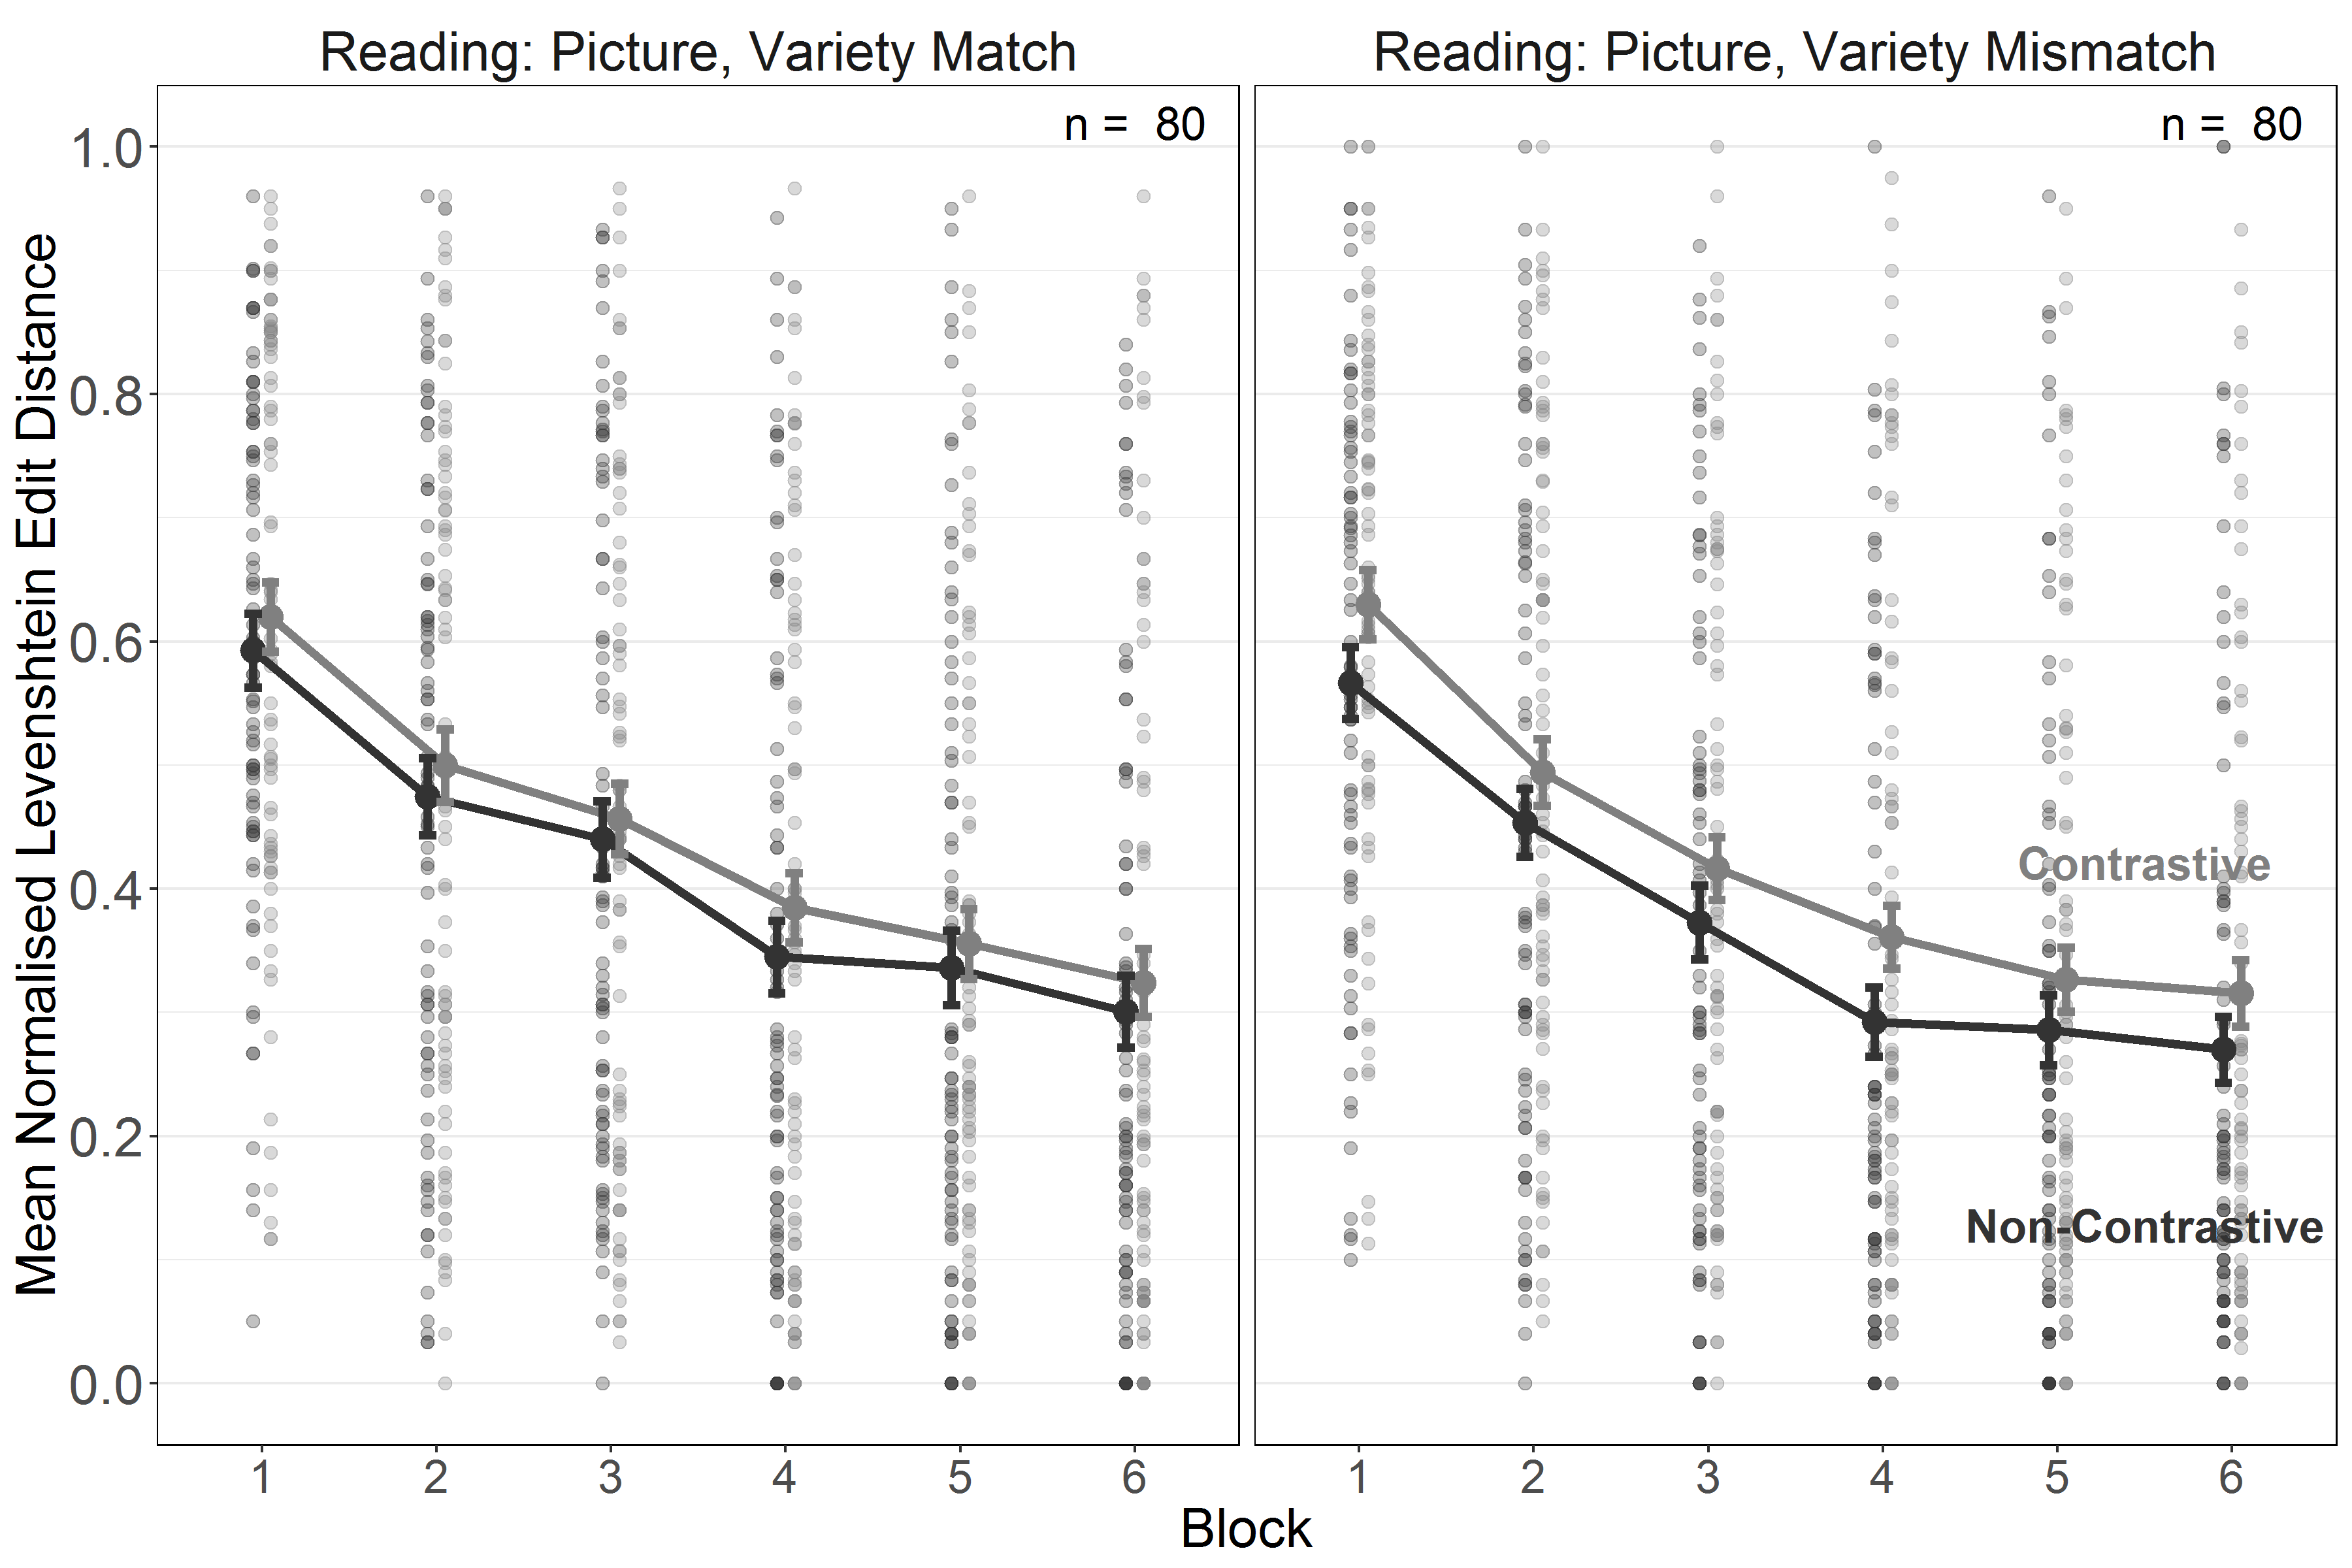
\includegraphics[width=1\linewidth]{C:/Users/g517364/Dropbox/GitHub/levenik/04_figures/output/experiment-3_training_plot_reading} 

}

\caption{Experiment 3. Length-normalised Levenshtein Edit Distance for reading of contrastive and non-contrastive words during 3 training blocks in the variety match and variety mismatch conditions. Error bars indicate $\pm$ 1 $SE$ of the mean.}\label{fig:ex3-train-reading-plots}
\end{figure}

\begin{figure}[htb]

{\centering 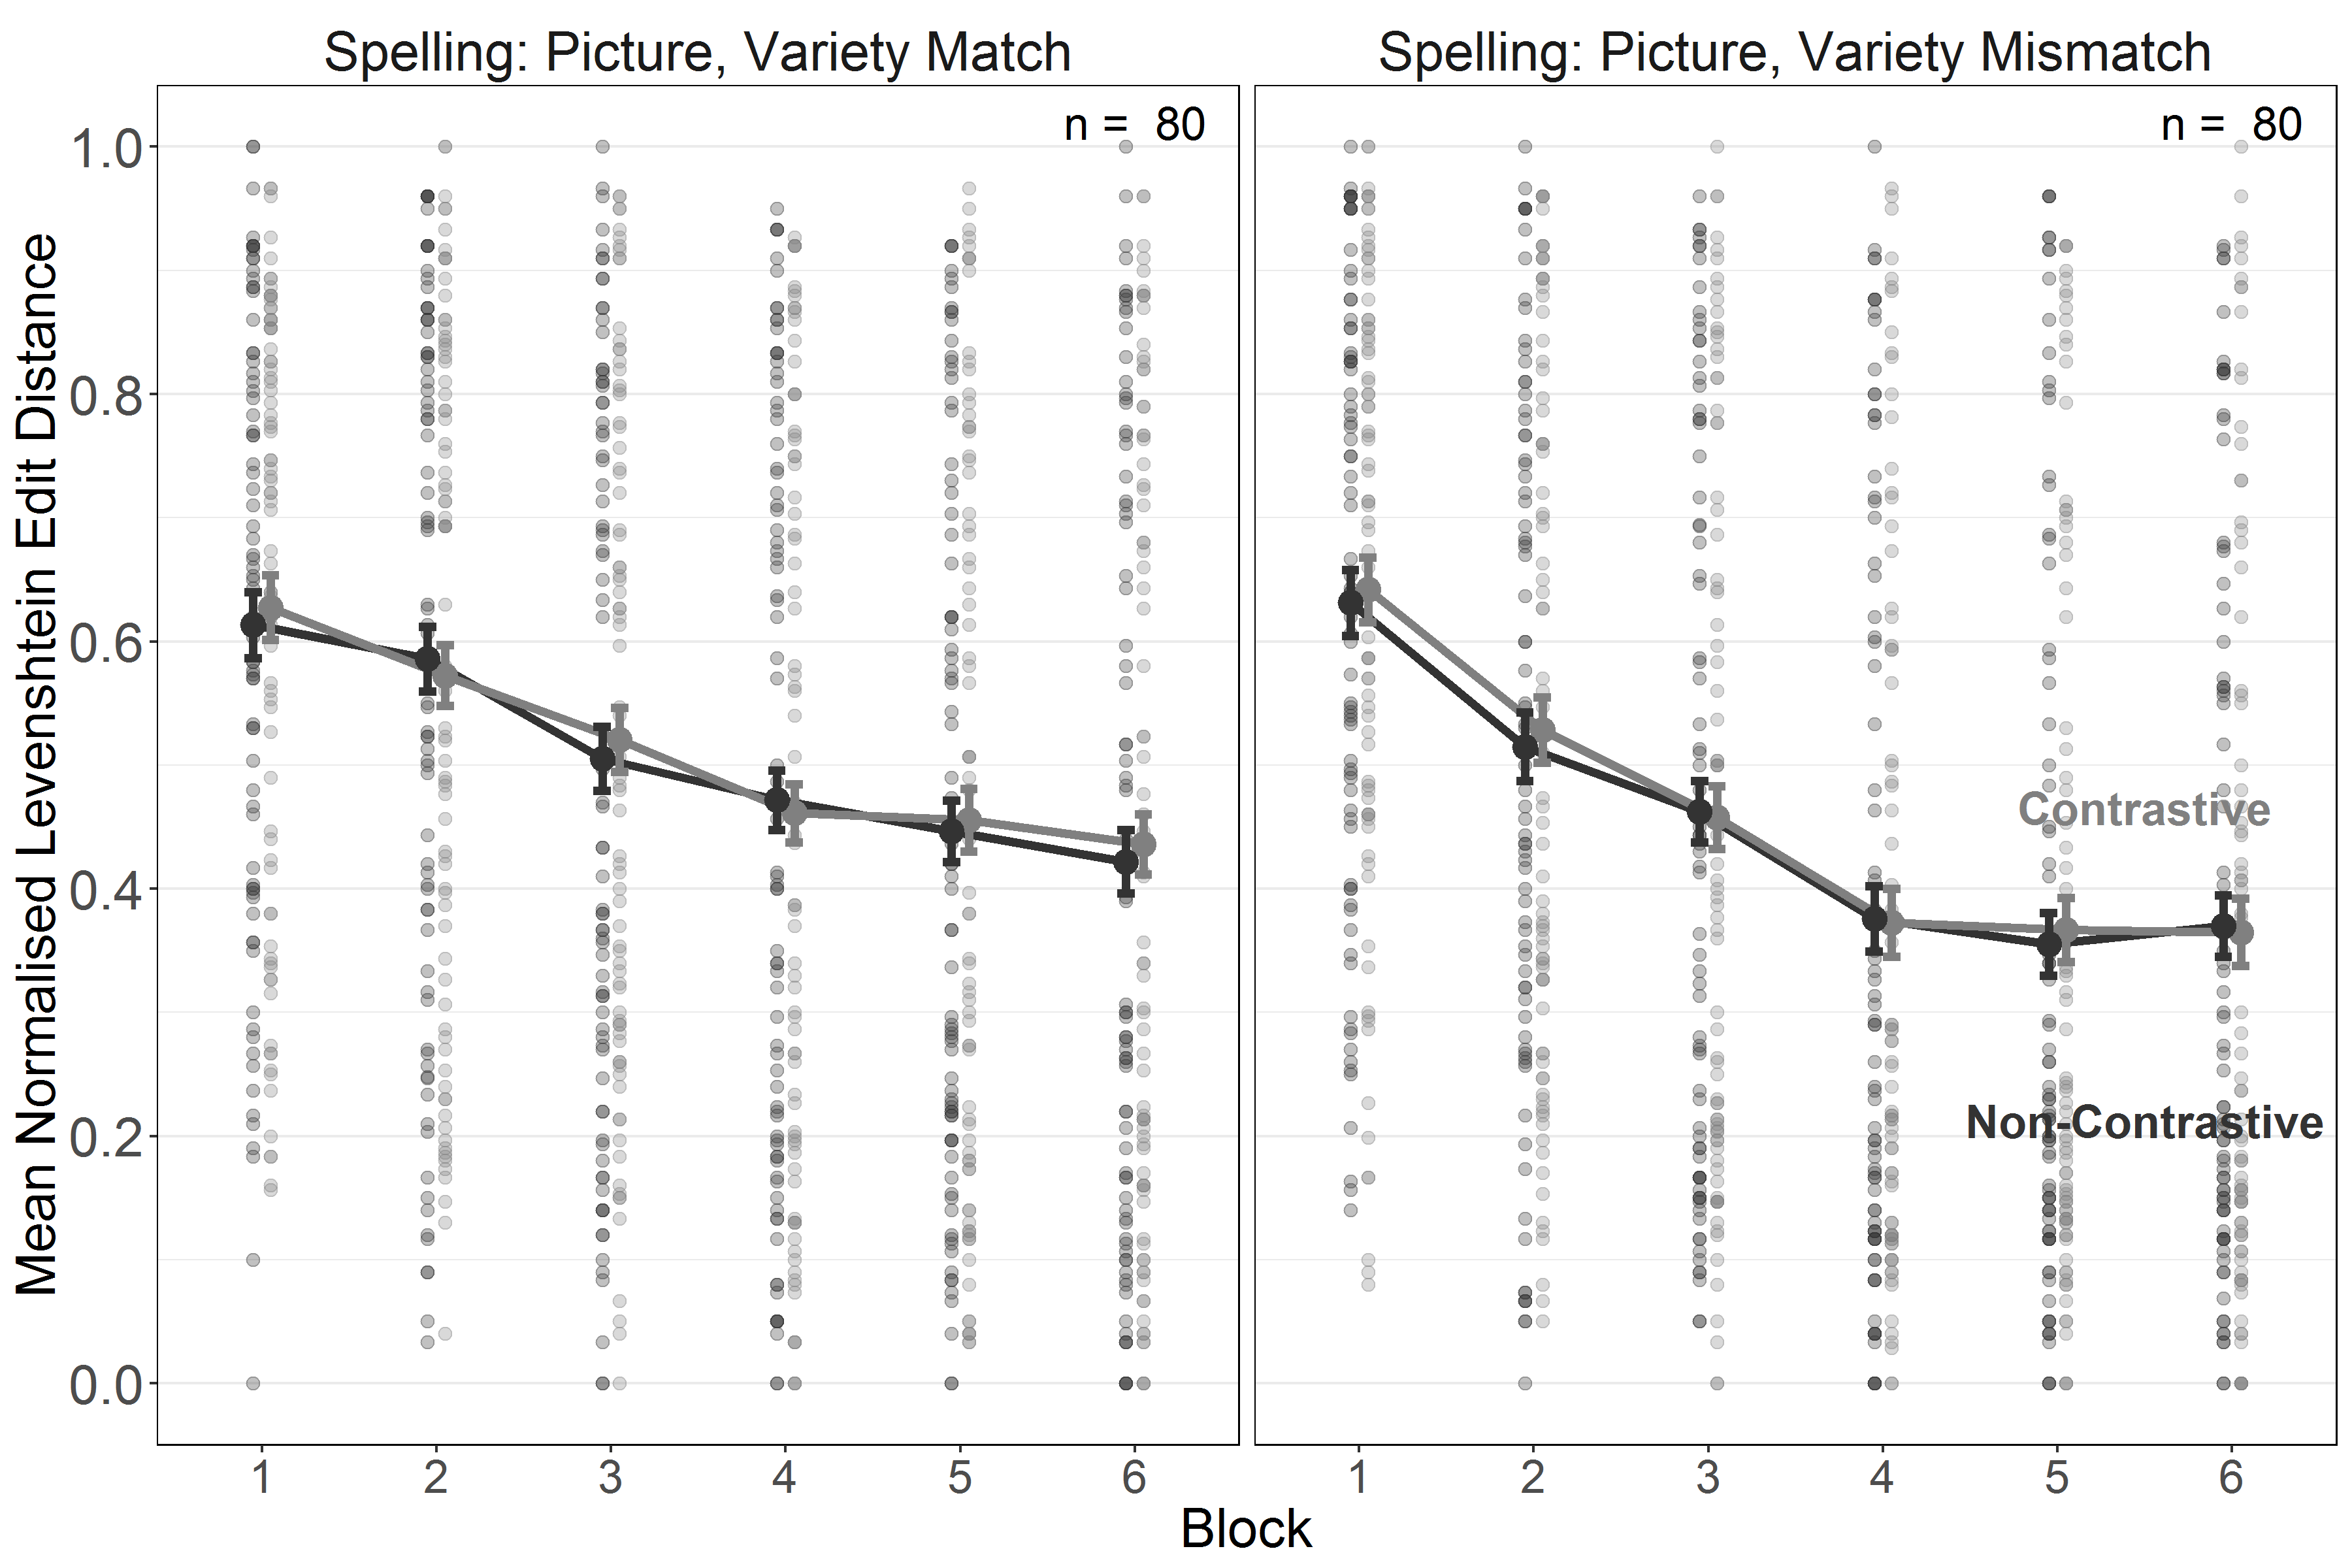
\includegraphics[width=1\linewidth]{C:/Users/g517364/Dropbox/GitHub/levenik/04_figures/output/experiment-3_training_plot_spelling} 

}

\caption{Experiment 3. Length-normalised Levenshtein Edit Distance for spelling of contrastive and non-contrastive words during 3 training blocks in the variety match and variety mismatch conditions. Error bars indicate $\pm$ 1 $SE$ of the mean.}\label{fig:ex3-train-spelling-plots}
\end{figure}

\paragraph{Testing}\label{testing-3}

Parameter estimates, confidence intervals (for the frequentist analysis)
and credible intervals (for the Bayesian analysis) are presented in
Table~\ref{tab:ex3-test} and depicted in
Figures~\ref{fig:ex3-test-reading-plots} and
\ref{fig:ex3-test-spelling-plots}.

\begin{table}[!h]

\caption{\label{tab:ex3-test}Experiment 3. Parameter estimates for the models fitted to nLEDs from the testing phase. Bayesian analyses report standardised parameter estimates (i.e. the intercept [grand mean] is centred at 0). Values of 0 with a sign indicate the direction of the estimate before rounding.}
\centering
\resizebox{\linewidth}{!}{
\fontsize{8}{10}\selectfont
\begin{tabular}{lrrlrlrrl}
\toprule
\multicolumn{1}{c}{ } & \multicolumn{5}{c}{Frequentist Estimates} & \multicolumn{3}{c}{Bayesian Estimates} \\
\cmidrule(l{3pt}r{3pt}){2-6} \cmidrule(l{3pt}r{3pt}){7-9}
Term & $Est.$ & $SE$ & 95\% Conf. I & $t$ & $p$ & $Est.$ & $SE$ & 95\% Cred. I\\
\midrule
Intercept & 0.58 & 0.03 & [0.51, 0.64] & 17.55 & < .001*** & 0.04 & 0.06 & [-0.08, 0.17]\\
\textbf{Task} & \textbf{-0.05} & \textbf{0.01} & \textbf{[-0.06, -0.03]} & \textbf{-5.75} & \textbf{< .001***} & \textbf{-0.09} & \textbf{0.02} & \textbf{[-0.12, -0.06]}\\
\textbf{Variety Condition} & \textbf{-0.07} & \textbf{0.03} & \textbf{[-0.12, -0.01]} & \textbf{-2.15} & \textbf{< .001***} & \textbf{-0.11} & \textbf{0.05} & \textbf{[-0.22, -0.01]}\\
TC $\times$ VC & 0.01 & 0.01 & [-0.00, 0.03] & 1.72 & < .001*** & 0.02 & 0.01 & [-0.00, 0.05]\\
\textbf{R, VMis: WT} & \textbf{-0.05} & \textbf{0.02} & \textbf{[-0.08, -0.02]} & \textbf{-2.86} & \textbf{< .001***} & \textbf{-0.09} & \textbf{0.03} & \textbf{[-0.16, -0.03]}\\
S, VMis: WT & 0.00 & 0.02 & [-0.04, 0.03] & -0.17 & 1.00 & 0.00 & 0.03 & [-0.06, 0.06]\\
R, VMa: WT & -0.03 & 0.02 & [-0.06, 0.01] & -1.58 & < .001*** & -0.05 & 0.03 & [-0.11, 0.02]\\
S, VMa: WT & -0.01 & 0.02 & [-0.04, 0.03] & -0.31 & 1.00 & -0.01 & 0.03 & [-0.07, 0.06]\\
R, VMis, WF & 0.02 & 0.01 & [-0.01, 0.04] & 1.11 & < .001*** & 0.03 & 0.03 & [-0.02, 0.09]\\
S, VMis, WF & -0.01 & 0.01 & [-0.03, 0.01] & -0.81 & < .001*** & -0.02 & 0.02 & [-0.07, 0.03]\\
\textbf{R, VMa, WF} & \textbf{0.04} & \textbf{0.01} & \textbf{[0.01, 0.07]} & \textbf{2.82} & \textbf{< .001***} & \textbf{0.07} & \textbf{0.03} & \textbf{[0.02, 0.13]}\\
S, VMa, WF & 0.00 & 0.01 & [-0.02, 0.02] & -0.13 & 1.00 & 0.00 & 0.02 & [-0.05, 0.04]\\
\bottomrule
\multicolumn{9}{l}{Variety Condition (VC) = variety match vs. variety mismatch (VMa vs. VMi),}\\
\multicolumn{9}{l}{Task Condition (TC) = reading vs. spelling (R vs. S),}\\
\multicolumn{9}{l}{Word Type (WT) = contrastive vs. non-contrastive, Word Familiarity (WF) = familiar vs. unfamiliar (novel)}\\
\end{tabular}}
\end{table}

As in the training data, there was a main effect of Task confirming
superior performance for reading compared to spelling and an effect of
Word Type, indicative of the contrastive deficit, for reading in the
Variety Mismatch condition. We also found that the effect of Word
Familiarity was significant for reading in the Variety Match condition
due to impaired performance for untrained compared to trained words in
this condition. Crucially, the analysis yielded a main effect of Variety
which showed that overall performance at test was superior in the
Variety Mismatch condition.

\begin{figure}[htb]

{\centering 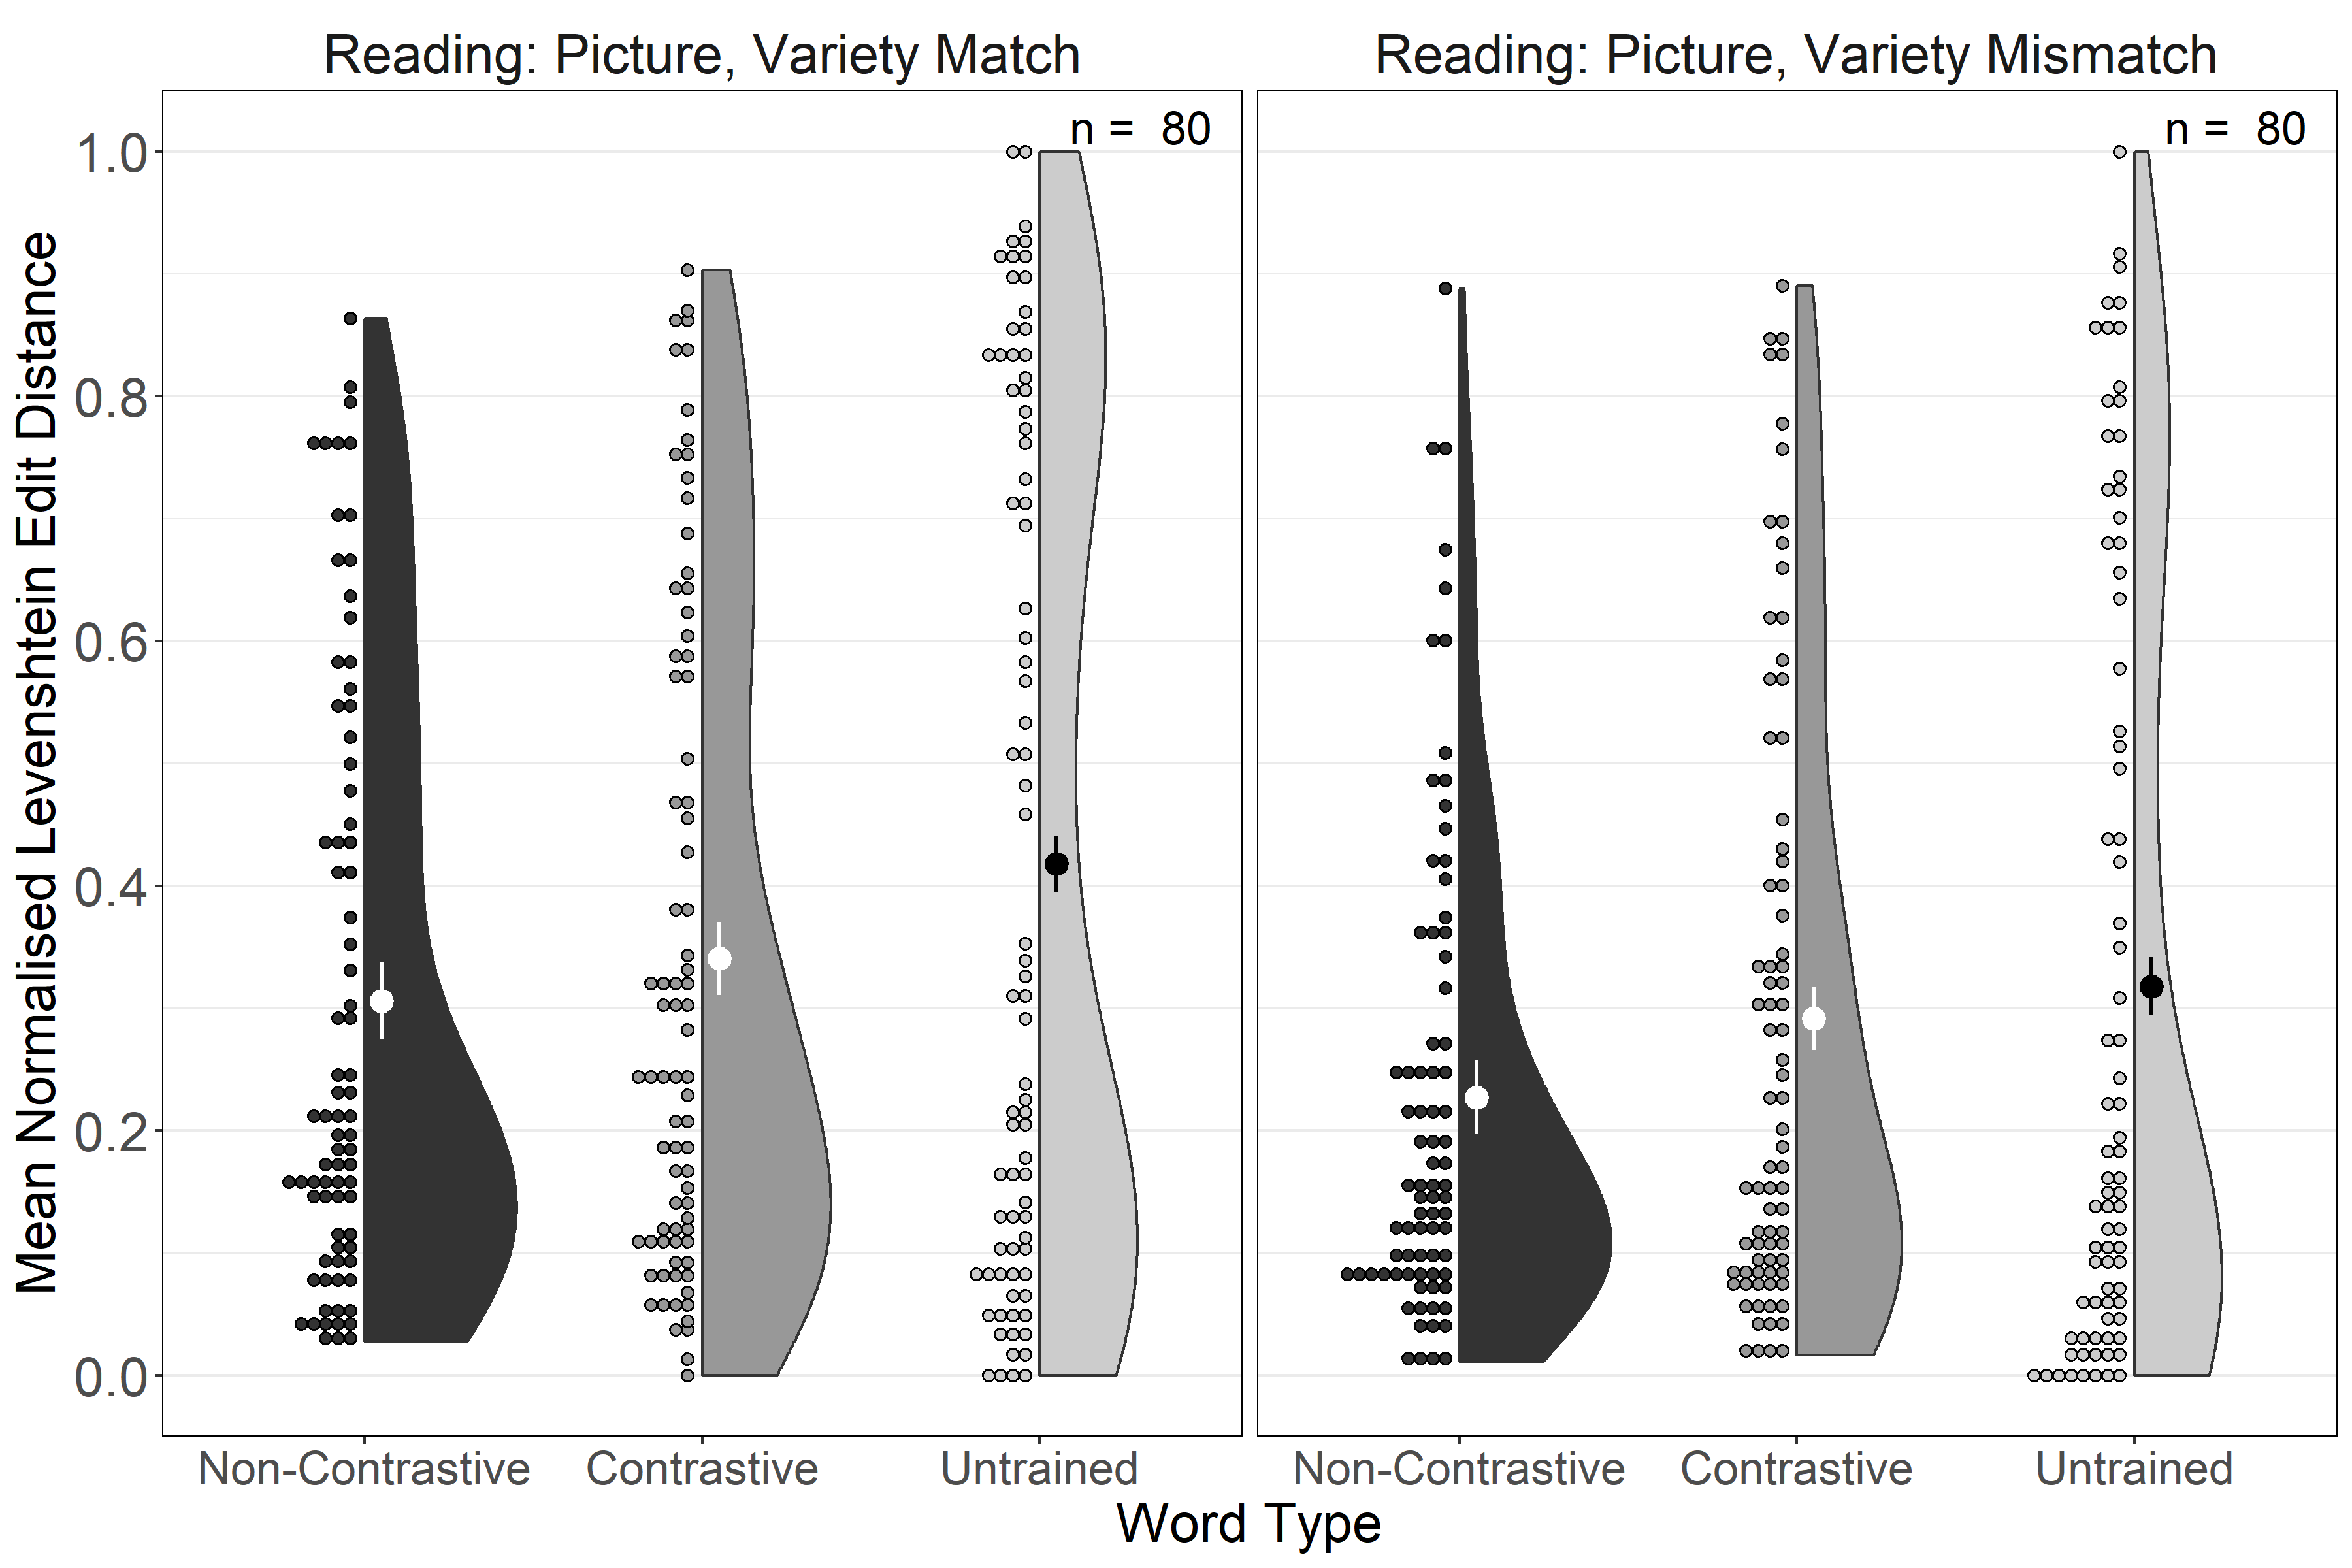
\includegraphics[width=1\linewidth]{C:/Users/g517364/Dropbox/GitHub/levenik/04_figures/output/experiment-3_testing_plot_reading} 

}

\caption{Experiment 3. Length-normalised Levenshtein Edit Distance for testing reading performance for trained non-contrastive, trained contrastive and untrained words in the variety match and variety mismatch conditions. Large dots and whiskers indicate means and $\pm$ 1 $SE$ of the mean.}\label{fig:ex3-test-reading-plots}
\end{figure}

\begin{figure}[htb]

{\centering 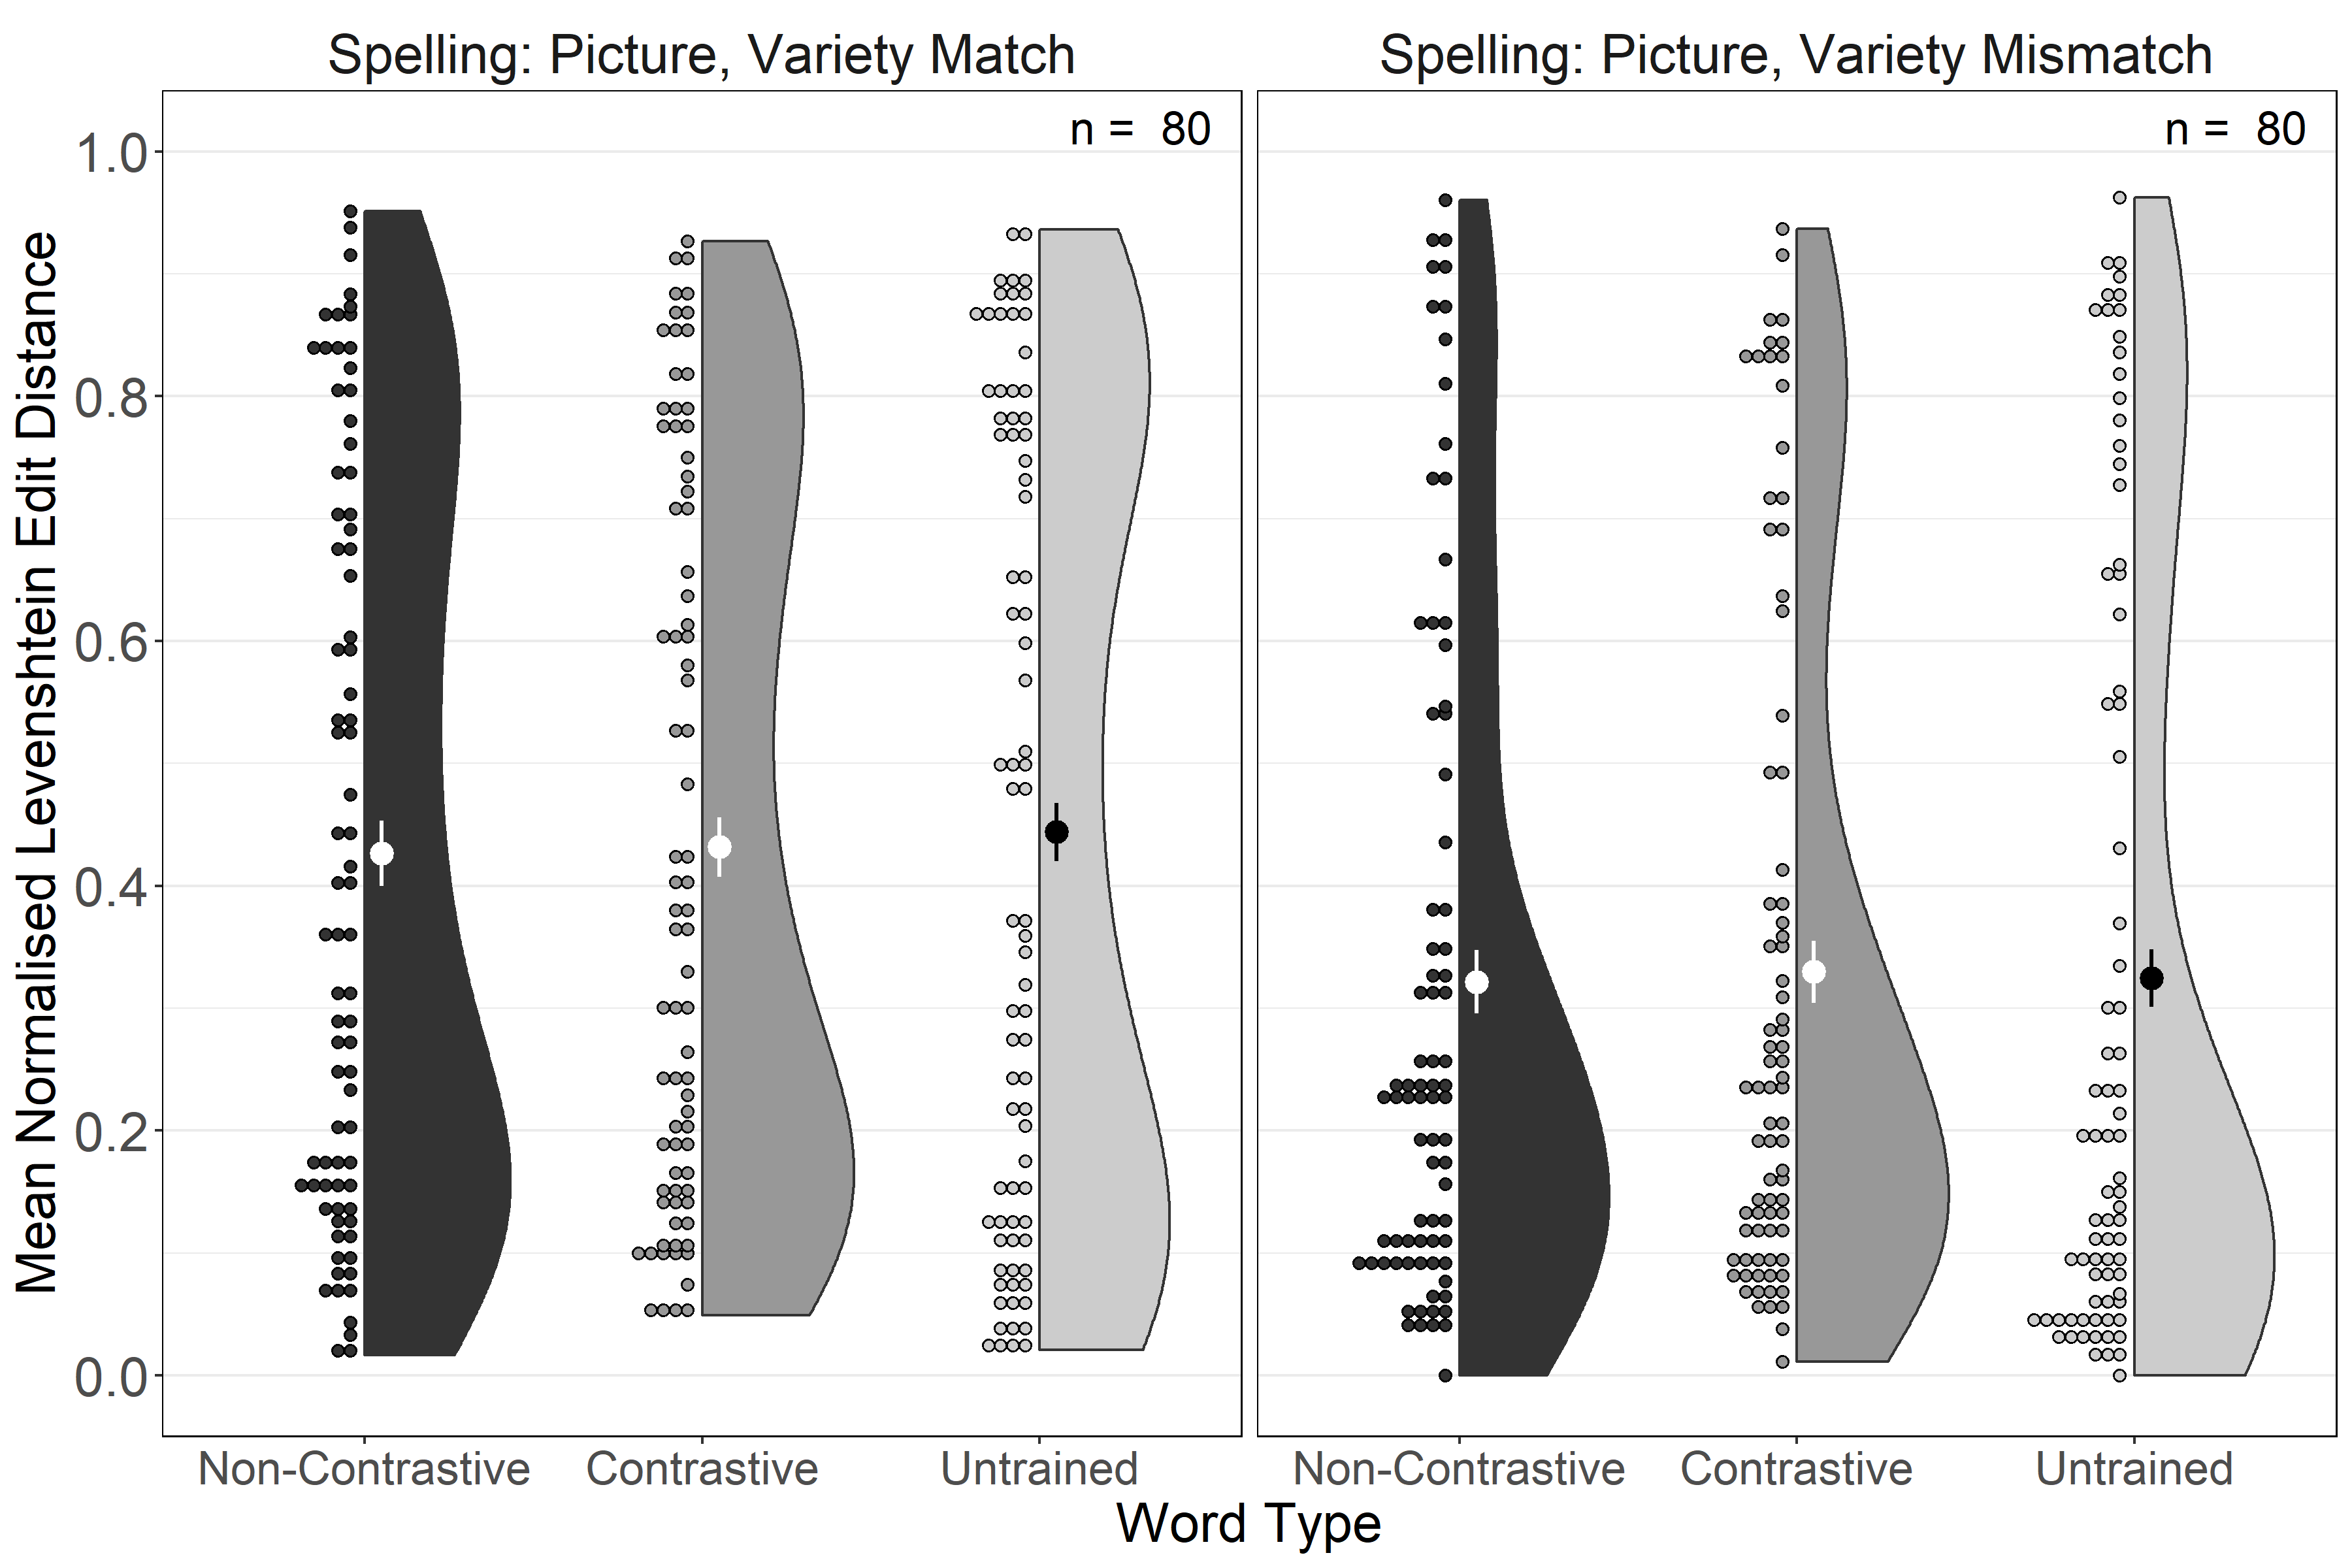
\includegraphics[width=1\linewidth]{C:/Users/g517364/Dropbox/GitHub/levenik/04_figures/output/experiment-3_testing_plot_spelling} 

}

\caption{Experiment 3. Length-normalised Levenshtein Edit Distance for testing spelling performance for trained non-contrastive, trained contrastive and untrained words in the variety match and variety mismatch conditions. Large dots and whiskers indicate means and $\pm$ 1 $SE$ of the mean.}\label{fig:ex3-test-spelling-plots}
\end{figure}

As in the previous experiments, we performed a planned comparison of
performance on untrained words only between the Variety Match and
Variety Mismatch conditions using the same model structure as in
Experiments 2a and 2b. The frequentist model yielded a significant
effect of Variety (\(\hat{\beta}\) = -0.08{[}-0.15, -0.01{]}, \emph{t} =
-2.20, \emph{p} = \textless{} .001***) with the Bayesian estimate
suggesting sufficient evidence in favour of this effect (\(\hat{\beta}\)
= -0.14{[}-0.26, -0.02{]}). This effect indicates that reading and
spelling performance was superior in the variety mismatch condition.

\subsection{Discussion}\label{discussion-3}

When a larger sample of participants was trained for twice as long as in
the previous experiments in reading and spelling of an opaque artificial
orthography of words for which semantic information was available there
was clear evidence for a contrastive deficit in reading in the Variety
Mismatch condition, both in training as well as in testing. This
indicates that when training is long enough for lexical and phonological
representations to be established exposure of competing variants that
are associated with the same meaning impairs reading. This contrastive
deficit could not have arisen had participants exclusively relied on a
phonics-based reading strategy that involved piecemeal conversion of
individual graphemes into the associated phonemes. In contrast, no
contrastive deficit emerged for spelling because no \enquote{dialect}
orthographic form had ever been presented and because spelling could
only be achieved through conversion of individual phonemes into the
associated graphemes.

At the same time, the Word Familiarity effect observed for reading in
the Variety Match condition suggests that when no competing variants
were encountered during literacy training participants seemed to rely
much more on trying to directly access the phonological forms of words,
either by converting the initial graphemes and accessing the ford form
based on initial segments or by accessing the word form based on the
meaning. Either processes would inevitably lead to impaired performance
with untrained words for which no phonological representations were
available, which is what we observed in this condition. The fact that no
effect of Word Familiarity was found for reading in the Variety Mismatch
condition suggests that when encountering competing variants
participants were less likely to access the word forms directly but
rather tried to assemble the words through sequential conversion of
graphemes into phonemes, i.e.~by pursuing a phonics-based reading
strategy. As a result, participants in the Variety Mismatch condition
exhibited an overall benefit in their literacy skills, especially for
untrained words.

\section{General Discussion}\label{general-discussion}

Our experiments compared a condition that simulated beginning readers'
encounter of different linguistic variants of words prior to literacy
acquisition with a condition in which no new variants are introduced, to
ascertain how exposure to more than one linguistic variety of the same
language might affect learning to read and to spell. Employing an
artificial language with an invented script allowed us to control for
potential confounds that often are associated with dialect exposure such
as differences in home literacy environment, cultural attitudes to
literacy or educational provision. Previous research (Brown et al.,
2015) had shown that encountering a variety mismatch impairs processing
of contrastive words, i.e.~words with different variants across
varieties such as Scots /hoose/ vs.~English /house/. What remained
unclear was whether impaired performance with these contrastive words is
also associated with a general deficit in literacy acquisition,
especially in learners' decoding abilities as measured by reading and
spelling of untrained words.

The results confirmed and extended the finding of a contrastive deficit
in children exposed to AAE reported by Brown et al. (2015). We
replicated this deficit and showed that it appeared most reliably when
pictures enabled participants to establish semantic representations
(Experiment 2a), when a transparent orthography made learning easier
(Experiment 2a) and There were no contrastive deficits in spelling.
Thus, when there was sufficient training to associate two variants with
the same meaning competition between these variants impairs reading but
not spelling. Even though the contrastive deficit in reading also
emerged in some instances when no pictures were present, it appeared
more consistently in conditions with pictures suggesting that shared
semantic representations seem to exacerbate the competition between
variants. This is in line with interactive activation and competition
models which place the locus of inhibition from high-frequency
competitors at the lexical layer. The existence of a semantic
representation will have reinforced this lexical competition via
bidirectional connections between lexical and semantic representations
(Chen \& Mirman, 2012). Thus, without a semantic layer, the
connectionist simulation reported by Brown et al. (2015) may even have
somewhat underestimated the degree of competition between dialect
variants of the same word. We predict that the addition of a semantic
layer to a connectionist model of this type should result in an even
more pronounced contrastive deficit.

The contrastive deficit differs from cognate facilitation effects in
bilingual word processing where the existence of a similar variant in
another language facilitates L1 and L2 reading due to
language-non-specific automatic co-activation of the phonologically
similar translation equivalent (Van Assche et al., 2009). It is
interesting to ponder in what ways bilingual and bi-dialectal readers
might differ in this regard. For example, it is conceivable that
something akin to cognate facilitation can emerge for contrastive words
at later stages of literacy acquisition under conditions of dialect
exposure when clear socially conditioned language-specific production
constraints, i.e.~a clear understanding as to where and when to use each
variety, are acquired. It is also possible that cognate facilitation in
bilingual readers emerges only if bilinguals are trained to read in both
languages, so that facilitation arises from partially or fully shared
graphemic representations. Future research will have to show whether
bi-dialectal individuals will start exhibiting facilitation for
contrastive words once they become proficient in selectively using each
of their varieties in appropriate contexts and situations, whether
facilitation only occurs when individuals learn to read in both
varieties or whether representations of languages vs.~dialects are
qualitatively different giving rise to different patterns of
co-activation and inhibition.

The existence of a contrastive deficit implies that readers attempt to
access word forms directly and not through grapheme-phoneme conversion.
This is because relying exclusively on a consecutive conversion of each
grapheme into the associated phoneme will inevitably lead correct
reading of the target word regardless of whether similar variants have
been encountered previously or not. We had hypothesised that
introduction of spelling training should attenuate the contrastive
deficit if it facilitates such phonologically mediated decoding
strategies (Taylor et al., 2017). However, we found that the contrastive
deficit in reading emerged even when spelling training was introduced.
Moreover, as the joint analyses of the first three experiments showed,
introducing spelling training did not lead to a significant improvement
in overall literacy nor in phonologically mediated decoding, in contrast
to studies demonstrating that invented, i.e.~non-normative spelling
facilitates reading by boosting phonemic awareness and by promoting an
analytical stance towards letter-sound correspondences (Ehri \& Wilce,
2006; G. P. Ouellette \& Sénéchal, 2008; G. Ouellette \& Sénéchal, 2017;
G. Ouellette, Sénéchal, \& August, 2008). This finding leads us to
conclude that adult learners, who already have mastered the alphabetic
principle, do not experience an additional boost from spelling training
but rather appear to maintain a separation of processing strategies for
reading and for spelling, relying more on direct access of word forms
during reading while converting phonemes into graphemes during spelling.
One possible explanation for why spelling did not boost phonologically
mediated decoding and, consequently, did not attenuate the contrastive
deficit in reading is that if conversion of individual phonemes into
graphemes and vice versa is perceived as effortful participants may rely
on this strategy only when there is no alternative, as in spelling, but
may prefer trying to access the phonological form -- either triggered by
decoded initial graphemes or directly from the depicted word meaning or
both -- whenever this alternative seems feasible, as it is in reading.
The fact that spelling performance was consistently worse than reading
performance confirms that systematic rule-based conversion is a more
effortful and hence more error-prone process. Thus, for adult learners,
acquiring literacy in a novel orthography appears to involve making
strategy choices, e.g.~between converting graphemes into phonemes
vs.~attempting to recall word forms from memory.

We had introduced testing of untrained words, which is the
artificial-language analogy to non-word reading tests for beginning
readers, to ascertain to what extent learners were able to generalise
phonologically mediated decoding skills. For reading, inferior
performance with untrained words could arise if participants had been
relying on memory-based retrieval of phonological forms with trained
words, a strategy that would then be unsuccessful for words they never
encountered before. Such retrieval may be triggered either by word
meaning as represented by the picture or by partial decoding that
provides access to the beginnings of the word's phonology. Conversely,
similar performance with trained and untrained words would indicate that
participants applied phonological decoding via grapheme-phoneme
conversion to a similar extent regardless of word familiarity. For
spelling, superior performance with trained words could only arise if
participants were able to directly retrieve representations of the
entire orthographic form, a possibility that is unlikely given the
complexity of our invented script, or if participants had acquired
knowledge of transitional probabilities between graphemes via
statistical learning of serial information, e.g.~about spatial locations
of letters on the on-screen keyboard and the associated motor routines.
We found that in those experiments where participants learned an opaque
orthography (Experiments 1, 2b, and 3), a familiarity benefit emerged
only for reading in the variety match condition when pictures were
present. This suggests that when faced with inconsistent mappings
between graphemes and phonemes, participants tried to capitalise as much
as possible on direct word form retrieval, yet this strategy was
attenuated when participants encountered competing variants, as the
absence of a word familiarity effect in the opaque orthography variety
mismatch conditions suggests. In contrast, in Experiment 2a, when
participants learned to read and spell a transparent orthography, the
familiarity effect was ubiquitous and emerged in almost all conditions
except in two of the spelling conditions, and even there the mean edit
distances pointed in the direction of better performance with familiar
words. The observed benefit for processing familiar words points towards
entrenchment of acquired decoding strategies when learning to read was
made easier by the transparent orthography -- regardless of whether it
relied on meaning-based access, partial phonological decoding, memory of
orthographic representations or serial information of motor routines
that underpinned keyboard-based spelling.

The crucial question of the present study was whether exposure to
different variants of some of the training words in the variety mismatch
conditions impaired decoding skills. In Experiments 1 and 2, Bayesian
analyses indicated that there was not sufficient evidence to decide,
neither with respect to overall performance nor with untrained words.
For the opaque orthography, this may simply have been due to the overall
difficulty of the task so that the absence of a variety mismatch effect
could be construed as due to a floor effect. But even for the
transparent orthography, where learning was more successful, there was
no evidence for a detrimental variety mismatch effect. However, when we
increased our sample size (presumably resulting in greater statistical
power) and extended the training phase in Experiment 3 we found a clear
performance benefit in the variety mismatch condition. This benefit was
significant for overall performance as well as for untrained words
separately, and provides clear evidence that under conditions mimicking
dialect exposure participants acquired superior decoding skills compared
to conditions that mimicked the absence of dialect variation.

What might account for such a dialect benefit in artificial literacy
acquisition? When discussing the differential performance in reading and
spelling we suggested that learners appear to make strategy choices
based on perceived difficulty. Specifically, reading, especially in
variety match conditions, may seem to be more easily achievable through
direct retrieval of memorised word forms. However, noticing greater
variety in the variety mismatch conditions may have diminished
participants' reliance on such a memory-based retrieval strategy during
reading and led them to favour a more rule-based, phonologically
mediated strategy. This push towards phonologically mediated reading,
triggered by greater variability in the input, seemed to have led to an
overall improvement in decoding skills. Thus, counter to expectations
formulated in the literature so far, our finding suggests that when all
other conditions are controlled dialect exposure may actually be
beneficial for literacy acquisition.

The finding of a dialect benefit comes with several caveats: First,
learners in this study were adults who already had acquired literacy in
one or more languages and were certainly familiar with the alphabetic
principle. Their prior literacy competence may have endowed them with
knowledge -- implicit or explicit -- of a variety of strategies they
could switch between depending on conditions. Such strategy choices may
not be available to children who are just starting on the path to
literacy using whatever strategies are emphasised in their educational
setting. Future research will have to investigate whether dialect
exposure may have similar benefits for children who are still just
learning about the different routes to reading and spelling.

Secondly, the artificial conditions of our study differ from
naturalistic literacy acquisition in several fundamental ways. For one,
the goal of learning in the conditions in which no pictures were present
was different from the typical goal of reading and spelling, which is to
access and to convey meaning. Here, all that participants were asked to
learn was the connection between print and sound, a limitation that was
motivated by our attempt to replicate the findings from the Brown et al.
(2015) connectionist simulations. Still, it may have shifted the
emphasis on access to phonological and graphemic representations more
than is appropriate in naturalistic literacy learning thereby affecting
the repertoire of strategies learners may have used. We had tried to
remedy this limitation by comparing these conditions with conditions in
which pictorial information about the meaning was available at all
times. However, unlike children, who typically know the meanings of the
words they try to read and spell, in these conditions our participants
learned the meaning of novel words at the same time as they learned to
read and spell. This is more akin to acquisition of a second language in
settings where learning is underpinned by print exposure, e.g.~when
adult learners learn a new language both from a teacher and a textbook
-- a more complex and potentially more effortful learning task. We had
tried to mitigate against this additional burden by providing pictorial
information about the meaning at all times but it is still possible that
this more difficult task may have proved taxing on attentional resources
and thereby altered learning strategies. To be able to generalise from
learning of artificial scripts to literacy acquisition by children,
future research may seek to investigate literacy acquisition under more
ecologically valid conditions, for example by using novel scripts with
familiar words.

Thirdly, our experiments provided no cues, social or otherwise, for
dialect use. All that participants encountered in the variety mismatch
conditions was greater variability in terms of variants, whether
associated with the same meaning or not. Yet dialect use is typically
associated with specific regional, social and situational constraints.
Brown et al. (2015), in their second simulation, showed that when
dialect variants were cued by context nodes coding for variety (AAE
vs.~MAE) the contrastive deficit was attenuated. This shows that
additional differentiating contextual information, provided consistently
alongside the phonologically similar variants, reduces competition in
line with an interactive activation and competition account that
explains competition from strong, and facilitation from weak(er),
competitors through inhibitory connections with non-linear activation
functions (Chen \& Mirman, 2012). Such an account may even allow for the
possibility that dialect variants turn from competing high frequency
neighbours into facilitating variety-tagged cognates as information
about the context of use is acquired and stored. Despite the lack of
contextual information, the present artificial language learning
experiments are still of relevance as some evidence suggests that,
unlike bilingual language acquisition, bi-dialectal sociolinguistic
competence in contextualising variation may take considerable time to
build, as indicated by the developmental trajectory for dialect
recognition (McCullough, Clopper, \& Wagner, 2019) and emergence of
social attitudes towards dialects (Kinzler \& DeJesus, 2013). One could
construe the situation simulated in these experiments as one in which
literacy acquisition precedes reliable acquisition of the
sociolinguistic competence that governs dialect use. In future studies,
we are planning to provide contextual information about each variety
alongside each of the different variants, which we predict should reduce
the difficulty with processing contrastive words. The intriguing
question is in what ways such contextual information affects learners'
strategy choices with respect to memorisation vs.~phonological
mediation.

Finally, we observed considerable variability in performance in all
reported experiments. A visual inspection of our figures suggests that
the distributions of edit distances to the target were bimodal in many
conditions. Even though the lack of a normal distribution of this
dependent variable does not preclude fitting the statistical models
described above, as the residuals were normally distributed in all
instances, it still point to qualitatively different strategies employed
by subgroups of our participants. These strategy choices may have been
influenced by individual differences in cognitive capacity and in
perception of task difficulty but may also reflect trade-offs between
expended effort and monetary gain unique to participants recruited on
crowdsourcing platforms, especially those who use these platforms
repeatedly as a source of income (El Maarry, Milland, \& Balke, 2018).
Specifically, the substantial duration of each experiment, in
conjunction with the reward offered in compliance with minimum wage
requirements, may have induced further effort-minimising strategies
beyond what would be expected in more naturalistic and potentially
better supervised literacy acquisition contexts. Although we tried to
mitigate against outright cheating (e.g.~note-taking) by placing time
constraints on different tasks, we still have to accept that some
participants may have expended too little effort for learning to occur.
Online artificial language learning studies of the kind conducted here
trade research convenience against greater variability in the interest
of testing large numbers of participants. Thus, our findings need to be
viewed in the context of the perhaps somewhat altered incentive
structure that arises from reward-based online research. We hope that
future research will be able to scrutinise whether our main finding of a
dialect benefit also holds in educational intervention studies.

\section{Conclusions}\label{conclusions}

In naturalistic contexts, it is difficult to disentangle dialect
exposure from other confounding factors that may adversely affect
literacy learning. The results from this artificial literacy learning
study using an invented script showed that while words with dialect
variants are more difficult to read, overall phonological decoding
skills can be facilitated if the increased variation in the input leads
learners to choose decoding strategies that involve grapheme-phoneme
conversion as a means of minimising memory load. Because such a
phonologically mediated pathway to literacy acquisition has been shown
to be essential in the early stages of learning to read and spell
(Castles et al., 2018; Taylor et al., 2017) our results -- if confirmed
in further studies with children -- raise the intriguing possibility
that dialect exposure may, in fact, yield tangible benefits for literacy
acquisition.

\newpage

\section{References}\label{references}

\begingroup
\setlength{\parindent}{-0.5in} \setlength{\leftskip}{0.5in}

\hypertarget{refs}{}
\hypertarget{ref-Apfelbaum2013}{}
Apfelbaum, K. S., Hazeltine, E., \& McMurray, B. (2013). Statistical
learning in reading: Variability in irrelevant letters helps children
learn phonics skills. \emph{Developmental Psychology}, \emph{49}(7),
1348--1365.
doi:\href{https://doi.org/10.1037/a0029839}{10.1037/a0029839}

\hypertarget{ref-Artiles2010}{}
Artiles, A. J., Kozleski, E. B., Osher, D., \& Ortiz, A. (2010).
Justifying and Explaining Disproportionality, 1968--2008: A Critique of
Underlying Views of Culture. \emph{Exceptional Children}, \emph{76}(3),
279--299.
doi:\href{https://doi.org/10.1177/001440291007600303}{10.1177/001440291007600303}

\hypertarget{ref-R-papaja}{}
Aust, F., \& Barth, M. (2018). \emph{papaja: Create APA manuscripts with
R Markdown}. Retrieved from \url{https://github.com/crsh/papaja}

\hypertarget{ref-Barr2013}{}
Barr, D. J., Levy, R., Scheepers, C., \& Tily, H. J. (2013). Random
effects structure for confirmatory hypothesis testing: Keep it maximal.
\emph{Journal of Memory and Language}, \emph{68}(3), 255--278.
doi:\href{https://doi.org/10.1016/j.jml.2012.11.001}{10.1016/j.jml.2012.11.001}

\hypertarget{ref-R-lme4}{}
Bates, D., Mächler, M., Bolker, B., \& Walker, S. (2015). Fitting linear
mixed-effects models using lme4. \emph{Journal of Statistical Software},
\emph{67}(1), 1--48.
doi:\href{https://doi.org/10.18637/jss.v067.i01}{10.18637/jss.v067.i01}

\hypertarget{ref-BBC2013}{}
BBC News. (2013). Colley Lane school in Halesowen bans Black Country
dialect. Retrieved from
\url{https://www.bbc.co.uk/news/uk-england-birmingham-24941692}

\hypertarget{ref-Boersma2017}{}
Boersma, P., \& Weenik, D. (2017). Praat: Doing phonetics by computer.
Retrieved from \url{http://praat.org/}

\hypertarget{ref-R-broom.mixed}{}
Bolker, B., \& Robinson, D. (n.d.). \emph{Broom.mixed: Tidying methods
for mixed models}. Retrieved from
\url{http://github.com/bbolker/broom.mixed}

\hypertarget{ref-Brown2015}{}
Brown, M. C., Sibley, D. E., Washington, J. A., Rogers, T. T., Edwards,
J. R., MacDonald, M. C., \& Seidenberg, M. S. (2015). Impact of dialect
use on a basic component of learning to read. \emph{Frontiers in
Psychology}, \emph{6}, 1--17.
doi:\href{https://doi.org/10.3389/fpsyg.2015.00196}{10.3389/fpsyg.2015.00196}

\hypertarget{ref-Buhler2018}{}
Bühler, J. C., Oertzen, T. von, McBride, C. A., Stoll, S., \& Maurer, U.
(2018). Influence of dialect use on early reading and spelling
acquisition in German-speaking children in Grade 1. \emph{Journal of
Cognitive Psychology}, \emph{30}(3), 336--360.
doi:\href{https://doi.org/10.1080/20445911.2018.1444614}{10.1080/20445911.2018.1444614}

\hypertarget{ref-R-brms_a}{}
Bürkner, P.-C. (2017). brms: An R package for Bayesian multilevel models
using Stan. \emph{Journal of Statistical Software}, \emph{80}(1), 1--28.
doi:\href{https://doi.org/10.18637/jss.v080.i01}{10.18637/jss.v080.i01}

\hypertarget{ref-R-brms_b}{}
Bürkner, P.-C. (2018). Advanced Bayesian multilevel modeling with the R
package brms. \emph{The R Journal}, \emph{10}(1), 395--411.

\hypertarget{ref-Burkner2019}{}
Bürkner, P.-C., \& Vuorre, M. (2019). Ordinal Regression Models in
Psychology: A Tutorial. \emph{Advances in Methods and Practices in
Psychological Science}, 1--25.
doi:\href{https://doi.org/10.1177/2515245918823199}{10.1177/2515245918823199}

\hypertarget{ref-Castles2018}{}
Castles, A., Rastle, K., \& Nation, K. (2018). Ending the Reading Wars:
Reading Acquisition From Novice to Expert. \emph{Psychological Science
in the Public Interest}, \emph{19}(1), 5--51.
doi:\href{https://doi.org/10.1177/1529100618772271}{10.1177/1529100618772271}

\hypertarget{ref-Changizi2005}{}
Changizi, M. A., \& Shimojo, S. (2005). Character complexity and
redundancy in writing systems over human history. \emph{Proceedings of
the Royal Society B}, \emph{272}, 267--75.
doi:\href{https://doi.org/10.1098/rspb.2004.2942}{10.1098/rspb.2004.2942}

\hypertarget{ref-Chen2012}{}
Chen, Q., \& Mirman, D. (2012). Competition and Cooperation Among
Similar Representations: Toward a Unified Account of Facilitative and
Inhibitory Effects of Lexical Neighbors. \emph{Psychological Review},
\emph{119}(2), 417--430.
doi:\href{https://doi.org/10.1037/a0027175}{10.1037/a0027175}

\hypertarget{ref-Coltheart2001}{}
Coltheart, M., Rastle, K., Perry, C., Langdon, R., \& Ziegler, J.
(2001). DRC: A dual route cascaded model of visual word recognition and
reading aloud. \emph{Psychological Review}, \emph{108}(1), 204--256.
doi:\href{https://doi.org/10.1037//0033-295x.108.1.204}{10.1037//0033-295x.108.1.204}

\hypertarget{ref-Crystal2003}{}
Crystal, D. (2003). \emph{The Cambridge encyclopedia of the English
language} (2nd ed.). Cambridge, UK: Cambridge University Press.

\hypertarget{ref-Cutler2008}{}
Cutler, L., \& Graham, S. (2008). Primary Grade Writing Instruction: A
National Survey. \emph{Journal of Educational Psychology},
\emph{100}(4), 907--919.
doi:\href{https://doi.org/10.1037/a0012656}{10.1037/a0012656}

\hypertarget{ref-DictionaryoftheScotsLanguage}{}
Dictionary of the Scots Language. (n.d.). Muckle. Retrieved from
\url{http://www.dsl.ac.uk/entry/snd/muckle}

\hypertarget{ref-Donaldson1999}{}
Donaldson, J. (1999). \emph{The Gruffalo}. Pan Macmillan.

\hypertarget{ref-Donaldson2005}{}
Donaldson, J. (2005). \emph{The Gruffalo's Child}. Pan Macmillan.

\hypertarget{ref-Ehri2006}{}
Ehri, L. C., \& Wilce, L. S. (2006). Does Learning to Spell Help
Beginners Learn to Read Words? \emph{Reading Research Quarterly},
\emph{22}(1), 47--65.
doi:\href{https://doi.org/10.2307/747720}{10.2307/747720}

\hypertarget{ref-ElMaarry2018}{}
El Maarry, K., Milland, K., \& Balke, W.-T. (2018). A Fair Share of the
Work ? The Evolving Ecosystem of Crowd Workers. In \emph{Proceedings of
the 10th acm conference on web science} (pp. 145--152).

\hypertarget{ref-Forsythe2017}{}
Forsythe, A., Street, N., \& Helmy, M. (2017). Revisiting Rossion and
Pourtois with new ratings for automated complexity, familiarity, beauty,
and encounter. \emph{Behavior Research Methods}, \emph{49}(4),
1484--1493.
doi:\href{https://doi.org/10.3758/s13428-016-0808-z}{10.3758/s13428-016-0808-z}

\hypertarget{ref-R-english}{}
Fox, J., Venables, B., Damico, A., \& Salverda, A. P. (2019).
\emph{English: Translate integers into english}. Retrieved from
\url{https://CRAN.R-project.org/package=english}

\hypertarget{ref-R-irr}{}
Gamer, M., Lemon, J., Fellows, I., \& Singh, P. (2019). \emph{Irr:
Various coefficients of interrater reliability and agreement}. Retrieved
from \url{https://CRAN.R-project.org/package=irr}

\hypertarget{ref-Gatlin2015}{}
Gatlin, B., \& Wanzek, J. (2015). Relations Among Children's Use of
Dialect and Literacy Skills: A Meta-Analysis. \emph{Journal of Speech,
Language, and Hearing Research}, \emph{58}, 1306--1318.
doi:\href{https://doi.org/10.1044/2015}{10.1044/2015}

\hypertarget{ref-Gottlob1999}{}
Gottlob, L. R., Goldinger, S. D., Stone, G. O., \& Van Orden, G. C.
(1999). Reading homographs: Orthographic, phonologic, and semantic
dynamics. \emph{Journal of Experimental Psychology: Human Perception and
Performance}, \emph{25}(2), 561--574.
doi:\href{https://doi.org/10.1037/0096-1523.25.2.561}{10.1037/0096-1523.25.2.561}

\hypertarget{ref-Harber1977}{}
Harber, J. R. (1977). Influence of presentation dialect and orthographic
form on reading performance of Black, inner-city children.
\emph{Educational Research Quarterly}, \emph{2}(2), 9--16.

\hypertarget{ref-Harley2006}{}
Harley, H. (2006). \emph{English words: A linguistic introduction}.
Oxford, UK: Blackwell Publishing.

\hypertarget{ref-Harm2004}{}
Harm, M. W., \& Seidenberg, M. S. (2004). Computing the meanings of
words in reading: Cooperative division of labor between visual and
phonological processes. \emph{Psychological Review}, \emph{111}(3),
662--720.
doi:\href{https://doi.org/10.1037/0033-295X.111.3.662}{10.1037/0033-295X.111.3.662}

\hypertarget{ref-Houghton2003}{}
Houghton, G., \& Zorzi, M. (2003). Normal and impaired spelling in a
connectionist dual-route architecture. \emph{Cognitive Neuropsychology},
\emph{20}(2), 115--162.
doi:\href{https://doi.org/10.1080/02643290242000871}{10.1080/02643290242000871}

\hypertarget{ref-Jared2012}{}
Jared, D., Cormier, P., Levy, B. A., \& Wade-Woolley, L. (2012).
Cross-language activation of phonology in young bilingual readers.
\emph{Reading and Writing}, \emph{25}(6), 1327--1343.
doi:\href{https://doi.org/10.1007/s11145-011-9320-0}{10.1007/s11145-011-9320-0}

\hypertarget{ref-GIMP1995}{}
Kimball, S., Mattis, P., \& The GIMP Development Team. (1995). GNU Image
Manipulation Program. Retrieved from \url{https://www.gimp.org/}

\hypertarget{ref-Kinzler2013}{}
Kinzler, K. D., \& DeJesus, J. M. (2013). Northern = smart and Southern
= nice: The development of accent attitudes in the United States.
\emph{Quarterly Journal of Experimental Psychology}, \emph{66}(6),
1146--1158.
doi:\href{https://doi.org/10.1080/17470218.2012.731695}{10.1080/17470218.2012.731695}

\hypertarget{ref-Koo2016}{}
Koo, T. K., \& Li, M. Y. (2016). A Guideline of Selecting and Reporting
Intraclass Correlation Coefficients for Reliability Research.
\emph{Journal of Chiropractic Medicine}, \emph{15}, 155--163.
doi:\href{https://doi.org/10.1016/j.jcm.2016.02.012}{10.1016/j.jcm.2016.02.012}

\hypertarget{ref-Kruschke2018}{}
Kruschke, J. K., \& Liddell, T. M. (2018). The Bayesian New Statistics:
Hypothesis testing, estimation, meta-analysis, and power analysis from a
Bayesian perspective. \emph{Psychonomic Bulletin and Review}, \emph{25},
178--206.
doi:\href{https://doi.org/10.3758/s13423-016-1221-4}{10.3758/s13423-016-1221-4}

\hypertarget{ref-R-lmerTest}{}
Kuznetsova, A., Brockhoff, P. B., \& Christensen, R. H. B. (2017).
lmerTest package: Tests in linear mixed effects models. \emph{Journal of
Statistical Software}, \emph{82}(13), 1--26.
doi:\href{https://doi.org/10.18637/jss.v082.i13}{10.18637/jss.v082.i13}

\hypertarget{ref-Labov1995}{}
Labov, W. (1995). Can reading failure be reversed? A linguistic approach
to the question. In V. L. Gadsden \& D. A. Wagner (Eds.), \emph{Literacy
among african american youth: Issues in learning, teaching, and
schooling} (pp. 39--68). Cresskill, NJ: Hampton Press.

\hypertarget{ref-R-emmeans}{}
Lenth, R. (2019). \emph{Emmeans: Estimated marginal means, aka
least-squares means}. Retrieved from
\url{https://CRAN.R-project.org/package=emmeans}

\hypertarget{ref-Marian2012}{}
Marian, V., Bartolotti, J., Chabal, S., \& Shook, A. (2012). Clearpond:
Cross-linguistic easy-access resource for phonological and orthographic
neighborhood densities. \emph{PLoS ONE}, \emph{7}(8), e43230.
doi:\href{https://doi.org/10.1371/journal.pone.0043230}{10.1371/journal.pone.0043230}

\hypertarget{ref-Mazzoni2016}{}
Mazzoni, D., \& Dannenberg, R. (2016). Audacity. Retrieved from
\url{http://audacityteam.org/}

\hypertarget{ref-McCullough2019}{}
McCullough, E. A., Clopper, C. G., \& Wagner, L. (2019). Regional
dialect perception across the lifespan: Identification and
discrimination. \emph{Language and Speech}, \emph{62}(1), 115--136.
doi:\href{https://doi.org/10.1177/0023830917743277}{10.1177/0023830917743277}

\hypertarget{ref-Milde2011}{}
Milde, B. (2011). Shapecatcher: Unicode character recognition. Retrieved
from \url{http://shapecatcher.com/}

\hypertarget{ref-Mirman2014}{}
Mirman, D. (2014). \emph{Growth Curve Analysis and Visualization Using
R} (p. 168). Boca Ranton, FL.: Chapman; Hall/CRC Press.

\hypertarget{ref-R-BayesFactor}{}
Morey, R. D., \& Rouder, J. N. (2018). \emph{BayesFactor: Computation of
bayes factors for common designs}. Retrieved from
\url{https://CRAN.R-project.org/package=BayesFactor}

\hypertarget{ref-R-here}{}
Müller, K. (2017). \emph{Here: A simpler way to find your files}.
Retrieved from \url{https://CRAN.R-project.org/package=here}

\hypertarget{ref-Nicenboim2016}{}
Nicenboim, B., \& Vasishth, S. (2016). Statistical methods for
linguistic research: Foundational Ideas---Part II. \emph{Linguistics and
Language Compass}, \emph{10}(11), 591--613.
doi:\href{https://doi.org/10.1111/lnc3.12207}{10.1111/lnc3.12207}

\hypertarget{ref-Ouellette2008b}{}
Ouellette, G. P., \& Sénéchal, M. (2008). A window into early literacy:
Exploring the cognitive and linguistic underpinnings of invented
spelling. \emph{Scientific Studies of Reading}, \emph{12}(2), 195--219.
doi:\href{https://doi.org/10.1080/10888430801917324}{10.1080/10888430801917324}

\hypertarget{ref-Ouellette2017}{}
Ouellette, G., \& Sénéchal, M. (2017). Invented spelling in kindergarten
as a predictor of reading and spelling in grade 1: A new pathway to
literacy, or just the same road, kess known? \emph{Developmental
Psychology}, \emph{53}(1), 77--88.
doi:\href{https://doi.org/10.1037/dev0000179}{10.1037/dev0000179}

\hypertarget{ref-Ouellette2008a}{}
Ouellette, G., Sénéchal, M., \& August, J. (2008). Pathways to Literacy:
A Study of Invented Spelling Its Role in Learning to Read and.
\emph{Child Development}, \emph{79}(4), 899--913.

\hypertarget{ref-Perry2007}{}
Perry, C., Ziegler, J. C., \& Zorzi, M. (2007). Nested incremental
modeling in the development of computational theories: The CDP+ model of
reading aloud. \emph{Psychological Review}, \emph{114}(2), 273--315.
doi:\href{https://doi.org/10.1037/0033-295X.114.2.273}{10.1037/0033-295X.114.2.273}

\hypertarget{ref-Perry2010}{}
Perry, C., Ziegler, J. C., \& Zorzi, M. (2010). Beyond single syllables:
Large-scale modeling of reading aloud with the Connectionist Dual
Process (CDP++) model. \emph{Cognitive Psychology}, \emph{61}, 106--151.
doi:\href{https://doi.org/10.1016/j.cogpsych.2010.04.001}{10.1016/j.cogpsych.2010.04.001}

\hypertarget{ref-Plaut1996}{}
Plaut, D. C., McClelland, J. L., Seidenberg, M. S., \& Patterson, K.
(1996). Understanding normal and impaired word reading: Computational
principles in quasi-regular domains. \emph{Psychological Review},
\emph{103}(1), 56--115.
doi:\href{https://doi.org/10.1037/0033-295X.103.1.56}{10.1037/0033-295X.103.1.56}

\hypertarget{ref-R-base}{}
R Core Team. (2018). \emph{R: A language and environment for statistical
computing}. Vienna, Austria: R Foundation for Statistical Computing.
Retrieved from \url{https://www.R-project.org/}

\hypertarget{ref-Rastle2019}{}
Rastle, K. (2019). EPS mid-career prize lecture 2017: Writing systems,
reading, and language. \emph{Quarterly Journal of Experimental
Psychology}, 1--16.
doi:\href{https://doi.org/10.1177/1747021819829696}{10.1177/1747021819829696}

\hypertarget{ref-Rodd2019}{}
Rodd, J. (2019). How to Maintain Data Quality When You Can't See Your
Participants. Retrieved from
\href{https://www.psychologicalscience.org/observer/how-to-maintain-data-quality-when-you-cant-see-your-participants\%7B/\#\%7D.XHzv5ldcHCF.twitter}{https://www.psychologicalscience.org/observer/how-to-maintain-data-quality-when-you-cant-see-your-participants\{\textbackslash{}\#\}.XHzv5ldcHCF.twitter}

\hypertarget{ref-Rossion2004}{}
Rossion, B., \& Pourtois, G. (2004). Revisiting Snodgrass and
Vanderwart's object pictorial set: The role of surface detail in
basic-level object recognition. \emph{Perception}, \emph{33}(2),
217--236. doi:\href{https://doi.org/10.1068/p5117}{10.1068/p5117}

\hypertarget{ref-Schad2018}{}
Schad, D. J., Hohenstein, S., Vasishth, S., \& Kliegl, R. (2018). How to
capitalize on a priori contrasts in linear (mixed) models: A tutorial.
\emph{arXiv Preprint arXiv:1807.10451.}

\hypertarget{ref-KSeymour2003}{}
Seymour, P. H. K., Aro, M., \& Erskine, J. M. (2003). Foundation
literacy acquisition in European orthographies. \emph{British Journal of
Psychology}, \emph{94}, 143--174. Retrieved from \url{www.bps.org.uk}

\hypertarget{ref-Steffensen1982}{}
Steffensen, M. S., Reynolds, R. E., McClure, E., \& Guthrie, L. F.
(1982). Black English Vernacular and reading comprehension: A cloze
study of third, sixth, and ninth graders. \emph{Journal of Reading
Behavior}, \emph{14}(3), 285--298.

\hypertarget{ref-Taylor2017}{}
Taylor, J. S. H., Davis, M. H., \& Rastle, K. (2017). Comparing and
Validating Methods of Reading Instruction Using Behavioural and Neural
Findings in an Artificial Orthography. \emph{Journal of Experimental
Psychology: General}, \emph{146}(6), 826--858.
doi:\href{https://doi.org/10.1037/xge0000301}{10.1037/xge0000301}

\hypertarget{ref-Taylor2011}{}
Taylor, J. S. H., Plunkett, K., \& Nation, K. (2011). The influence of
consistency, frequency, and semantics on learning to read: An artificial
orthography paradigm. \emph{Journal of Experimental Psychology:
Learning, Memory, and Cognition}, \emph{37}(1), 60--76.
doi:\href{https://doi.org/10.1037/a0020126}{10.1037/a0020126}

\hypertarget{ref-VanAssche2009}{}
Van Assche, E., Duyck, W., Hartsuiker, R. J., \& Diependaele, K. (2009).
Does Bilingualism Change Native-Language Reading? Cognate Effects in a
Sentence Context. \emph{Psychological Science}, \emph{20}(8), 923--927.

\hypertarget{ref-Vasishth2018}{}
Vasishth, S., Mertzen, D., Jäger, L. A., \& Gelman, A. (2018). The
statistical significance filter leads to overoptimistic expectations of
replicability. \emph{Journal of Memory and Language},
\emph{103}(August), 151--175.
doi:\href{https://doi.org/10.1016/j.jml.2018.07.004}{10.1016/j.jml.2018.07.004}

\hypertarget{ref-Vidal2017}{}
Vidal, C., Content, A., \& Chetail, F. (2017). BACS: The Brussels
Artificial Character Sets for studies in cognitive psychology and
neuroscience. \emph{Behavior Research Methods}, \emph{49}(6),
2093--2112.
doi:\href{https://doi.org/10.3758/s13428-016-0844-8}{10.3758/s13428-016-0844-8}

\hypertarget{ref-R-tidyverse}{}
Wickham, H. (2017). \emph{Tidyverse: Easily install and load the
'tidyverse'}. Retrieved from
\url{https://CRAN.R-project.org/package=tidyverse}

\hypertarget{ref-R-knitr}{}
Xie, Y. (2015). \emph{Dynamic documents with R and knitr} (2nd ed.).
Boca Raton, Florida: Chapman; Hall/CRC. Retrieved from
\url{https://yihui.name/knitr/}

\hypertarget{ref-R-kableExtra}{}
Zhu, H. (2019). \emph{KableExtra: Construct complex table with 'kable'
and pipe syntax}. Retrieved from
\url{https://CRAN.R-project.org/package=kableExtra}

\endgroup

\clearpage



\begin{appendix}
\section{}
\subsection{Appendix A. Graphemes used to render phonemes in all
experiments.}\label{appendix-a}

\begin{figure}[htb]

{\centering 
\includegraphics[width=0.1\linewidth,height=0.2\textheight]{C:/Users/g517364/Dropbox/GitHub/levenik/01_materials/images/script/script_PNG/1} 
\includegraphics[width=0.1\linewidth,height=0.2\textheight]{C:/Users/g517364/Dropbox/GitHub/levenik/01_materials/images/script/script_PNG/2} 
\includegraphics[width=0.1\linewidth,height=0.2\textheight]{C:/Users/g517364/Dropbox/GitHub/levenik/01_materials/images/script/script_PNG/3} 
\includegraphics[width=0.1\linewidth,height=0.2\textheight]{C:/Users/g517364/Dropbox/GitHub/levenik/01_materials/images/script/script_PNG/4} 
\includegraphics[width=0.1\linewidth,height=0.2\textheight]{C:/Users/g517364/Dropbox/GitHub/levenik/01_materials/images/script/script_PNG/5} 
\includegraphics[width=0.1\linewidth,height=0.2\textheight]{C:/Users/g517364/Dropbox/GitHub/levenik/01_materials/images/script/script_PNG/6} 
\includegraphics[width=0.1\linewidth,height=0.2\textheight]{C:/Users/g517364/Dropbox/GitHub/levenik/01_materials/images/script/script_PNG/7} 
\includegraphics[width=0.1\linewidth,height=0.2\textheight]{C:/Users/g517364/Dropbox/GitHub/levenik/01_materials/images/script/script_PNG/8} 
\includegraphics[width=0.1\linewidth,height=0.2\textheight]{C:/Users/g517364/Dropbox/GitHub/levenik/01_materials/images/script/script_PNG/9} 
\includegraphics[width=0.1\linewidth,height=0.2\textheight]{C:/Users/g517364/Dropbox/GitHub/levenik/01_materials/images/script/script_PNG/10} 
\includegraphics[width=0.1\linewidth,height=0.2\textheight]{C:/Users/g517364/Dropbox/GitHub/levenik/01_materials/images/script/script_PNG/11} 
\includegraphics[width=0.1\linewidth,height=0.2\textheight]{C:/Users/g517364/Dropbox/GitHub/levenik/01_materials/images/script/script_PNG/12} 
\includegraphics[width=0.1\linewidth,height=0.2\textheight]{C:/Users/g517364/Dropbox/GitHub/levenik/01_materials/images/script/script_PNG/13} 
\includegraphics[width=0.1\linewidth,height=0.2\textheight]{C:/Users/g517364/Dropbox/GitHub/levenik/01_materials/images/script/script_PNG/14} 
\includegraphics[width=0.1\linewidth,height=0.2\textheight]{C:/Users/g517364/Dropbox/GitHub/levenik/01_materials/images/script/script_PNG/15} 

}

\caption{Invented graphemes used to represent each phoneme in all experiments. Note: The final two items were created but unused in this series of studies.}\label{fig:unnamed-chunk-5}
\end{figure}
\end{appendix}

\clearpage



\begin{appendix}
\section{}
\subsection{Appendix C. The Gruffalo books.}\label{appendix-b}

\subsubsection{The Gruffalo}\label{the-gruffalo}

\begin{itemize}
\tightlist
\item
  The Doric Gruffalo (translated by Sheena Blackhall)
\item
  Thi Dundee Gruffalo (translated by Matthew Fitt)
\item
  The Glasgow Gruffalo (translated by Elaine C. Smith)
\item
  The Gruffalo in Scots (translated by James Robertson)
\end{itemize}

\subsubsection{The Gruffalo's Child}\label{the-gruffalos-child}

\begin{itemize}
\tightlist
\item
  The Doric Gruffalo's Bairn (translated by Sheena Blackhall)
\item
  Thi Dundee Gruffalo's Bairn (translated by Matthew Fitt)
\item
  The Gruffalo's Wean (Scots; translated by James Robertson)
\end{itemize}

Note: The Gruffalo's Child was not available in Glaswegian during
creation of this corpus analysis.
\end{appendix}

\clearpage



\begin{appendix}
\section{}
\subsection{Appendix D. List of words and their
variants.}\label{appendix-c}

\begin{table}[!h]

\caption{\label{tab:unnamed-chunk-6}Word list used in all experiments. Experiment 1, 2b, and 3 use the opaque pronunciations, while Experiment 2a uses the transparent pronunciations.}
\centering
\fontsize{8}{10}\selectfont
\begin{tabular}{llll}
\toprule
\multicolumn{2}{c}{Spelling} & \multicolumn{2}{c}{Pronunciation} \\
\cmidrule(l{3pt}r{3pt}){1-2} \cmidrule(l{3pt}r{3pt}){3-4}
Transaprent & Opaque & Non-Contrastive & Contrastive\\
\midrule
mab & mab & mab & \\
skub & skub & skub & \\
klEb & klEb & klEb & \\
dOlk & dOlk & dOlk & \\
suld & suld & suld & \\
dikla & dikla & dikla & \\
luskO & luskO & luskO & \\
klufE & klufE & klufE & \\
klOda & klOda & klOda & \\
skOnEf & skOnEf & skOnEf & \\
klusim & klusim & klusim & \\
flabun & flabun & flabun & \\
nEsk & nEsk & nEsk & nisx\\
skEfi & skEfi & skEfi & sxifi\\
blEkus & bnEkus & blEkus & blixus\\
flEsOd & flEsOd & flEsOd & flisO\\
nEf & nEf & nEf & nif\\
bEsmi & bEsmi & bEsmi & bismi\\
nal & nal & nal & nOl\\
daf & daf & daf & dOf\\
blaf & bnaf & blaf & blOf\\
balf & balf & balf & bOlf\\
dasmu & dasmu & dasmu & dOsmu\\
smadu & smadu & smadu & smOdu\\
kublE & kubnE & kublE & xublE\\
slOku & fnOku & slOku & slOxu\\
snid & fnid & snid & sni\\
fub & fub & fub & \\
mif & mif & mif & \\
lOm & lOm & lOm & \\
snOf & fnOf & snOf & \\
blim & bnim & blim & \\
flOb & flOb & flOb & \\
mOls & mOls & mOls & \\
fOns & fOns & fOns & \\
nifs & nifs & nifs & \\
nOflE & nOflE & nOflE & \\
dEsna & dEfna & dEsna & \\
smiba & smiba & smiba & \\
flidu & flidu & flidu & \\
snibOl & fnibOl & snibOl & \\
slinab & fninab & slinab & \\
\bottomrule
\end{tabular}
\end{table}
\end{appendix}

\clearpage



\begin{appendix}
\section{}
\subsection{Appendix E. Images used from the Rossion and Pourtois (2004)
picture set and their related norming results.}\label{appendix-d}

We selected a subset of the items from the freely available colorised
Vanderwart image set (Rossion \& Pourtois, 2004). These are as follows:

\begin{itemize}
\item
  Body part: Finger, foot, eye, hand, nose, arm, ear.
\item
  Furniture and kitchen utensils: Chair, glass, bed, fork, spoon, pot,
  desk.
\item
  Household objects, tools, and instruments: Television, toothbrush,
  book, pen, refrigerator, watch, pencil.
\item
  Food and clothing: Pants, socks, shirt, sweater, apple, tomato,
  potato.
\item
  Buildings, building features, and vehicles: Door, house, window, car,
  doorknob, truck, bicycle. Animals and plants: Tree, dog, cat, flower,
  rabbit, duck, chicken.
\end{itemize}

The subset of pictures and their associated norms are provided in the
supplemental material at \url{https://osf.io/5mtdj/}.
\end{appendix}


\end{document}
